% Options for packages loaded elsewhere
\PassOptionsToPackage{unicode}{hyperref}
\PassOptionsToPackage{hyphens}{url}
%
\documentclass[
  ignorenonframetext,
]{beamer}
\usepackage{pgfpages}
\setbeamertemplate{caption}[numbered]
\setbeamertemplate{caption label separator}{: }
\setbeamercolor{caption name}{fg=normal text.fg}
\beamertemplatenavigationsymbolsempty
% Prevent slide breaks in the middle of a paragraph
\widowpenalties 1 10000
\raggedbottom
\setbeamertemplate{part page}{
  \centering
  \begin{beamercolorbox}[sep=16pt,center]{part title}
    \usebeamerfont{part title}\insertpart\par
  \end{beamercolorbox}
}
\setbeamertemplate{section page}{
  \centering
  \begin{beamercolorbox}[sep=12pt,center]{part title}
    \usebeamerfont{section title}\insertsection\par
  \end{beamercolorbox}
}
\setbeamertemplate{subsection page}{
  \centering
  \begin{beamercolorbox}[sep=8pt,center]{part title}
    \usebeamerfont{subsection title}\insertsubsection\par
  \end{beamercolorbox}
}
\AtBeginPart{
  \frame{\partpage}
}
\AtBeginSection{
  \ifbibliography
  \else
    \frame{\sectionpage}
  \fi
}
\AtBeginSubsection{
  \frame{\subsectionpage}
}
\usepackage{amsmath,amssymb}
\usepackage{lmodern}
\usepackage{iftex}
\ifPDFTeX
  \usepackage[T1]{fontenc}
  \usepackage[utf8]{inputenc}
  \usepackage{textcomp} % provide euro and other symbols
\else % if luatex or xetex
  \usepackage{unicode-math}
  \defaultfontfeatures{Scale=MatchLowercase}
  \defaultfontfeatures[\rmfamily]{Ligatures=TeX,Scale=1}
\fi
\usetheme[]{Frankfurt}
\usecolortheme{beaver}
% Use upquote if available, for straight quotes in verbatim environments
\IfFileExists{upquote.sty}{\usepackage{upquote}}{}
\IfFileExists{microtype.sty}{% use microtype if available
  \usepackage[]{microtype}
  \UseMicrotypeSet[protrusion]{basicmath} % disable protrusion for tt fonts
}{}
\makeatletter
\@ifundefined{KOMAClassName}{% if non-KOMA class
  \IfFileExists{parskip.sty}{%
    \usepackage{parskip}
  }{% else
    \setlength{\parindent}{0pt}
    \setlength{\parskip}{6pt plus 2pt minus 1pt}}
}{% if KOMA class
  \KOMAoptions{parskip=half}}
\makeatother
\usepackage{xcolor}
\IfFileExists{xurl.sty}{\usepackage{xurl}}{} % add URL line breaks if available
\IfFileExists{bookmark.sty}{\usepackage{bookmark}}{\usepackage{hyperref}}
\hypersetup{
  pdftitle={Spatial autocorrelation},
  pdfauthor={Vojtěch Barták},
  hidelinks,
  pdfcreator={LaTeX via pandoc}}
\urlstyle{same} % disable monospaced font for URLs
\newif\ifbibliography
\usepackage{graphicx}
\makeatletter
\def\maxwidth{\ifdim\Gin@nat@width>\linewidth\linewidth\else\Gin@nat@width\fi}
\def\maxheight{\ifdim\Gin@nat@height>\textheight\textheight\else\Gin@nat@height\fi}
\makeatother
% Scale images if necessary, so that they will not overflow the page
% margins by default, and it is still possible to overwrite the defaults
% using explicit options in \includegraphics[width, height, ...]{}
\setkeys{Gin}{width=\maxwidth,height=\maxheight,keepaspectratio}
% Set default figure placement to htbp
\makeatletter
\def\fps@figure{htbp}
\makeatother
\setlength{\emergencystretch}{3em} % prevent overfull lines
\providecommand{\tightlist}{%
  \setlength{\itemsep}{0pt}\setlength{\parskip}{0pt}}
\setcounter{secnumdepth}{-\maxdimen} % remove section numbering
\AtBeginSubsection{}
\ifLuaTeX
  \usepackage{selnolig}  % disable illegal ligatures
\fi

\title{Spatial autocorrelation}
\author{Vojtěch Barták}
\date{LS 2022}

\begin{document}
\frame{\titlepage}

\begin{frame}[allowframebreaks]
  \tableofcontents[hideallsubsections]
\end{frame}
\hypertarget{spatial-autocorrelation-and-why-it-matters}{%
\section{Spatial autocorrelation and why it
matters}\label{spatial-autocorrelation-and-why-it-matters}}

\hypertarget{types-of-data-in-spatial-statistics}{%
\subsection{Types of data in spatial
statistics}\label{types-of-data-in-spatial-statistics}}

\begin{frame}{Types of data in spatial statistics}
\begin{itemize}
\tightlist
\item
  Geostatistical data
\item
  Point pattern data
\item
  Areal (lattice) data
\end{itemize}
\end{frame}

\hypertarget{problem-with-spatially-autocorrelated-data}{%
\subsection{Problem with spatially autocorrelated
data}\label{problem-with-spatially-autocorrelated-data}}

\begin{frame}{Problem with spatially autocorrelated data}
\small

\textbf{Spatial} or \textbf{structural} relationship?

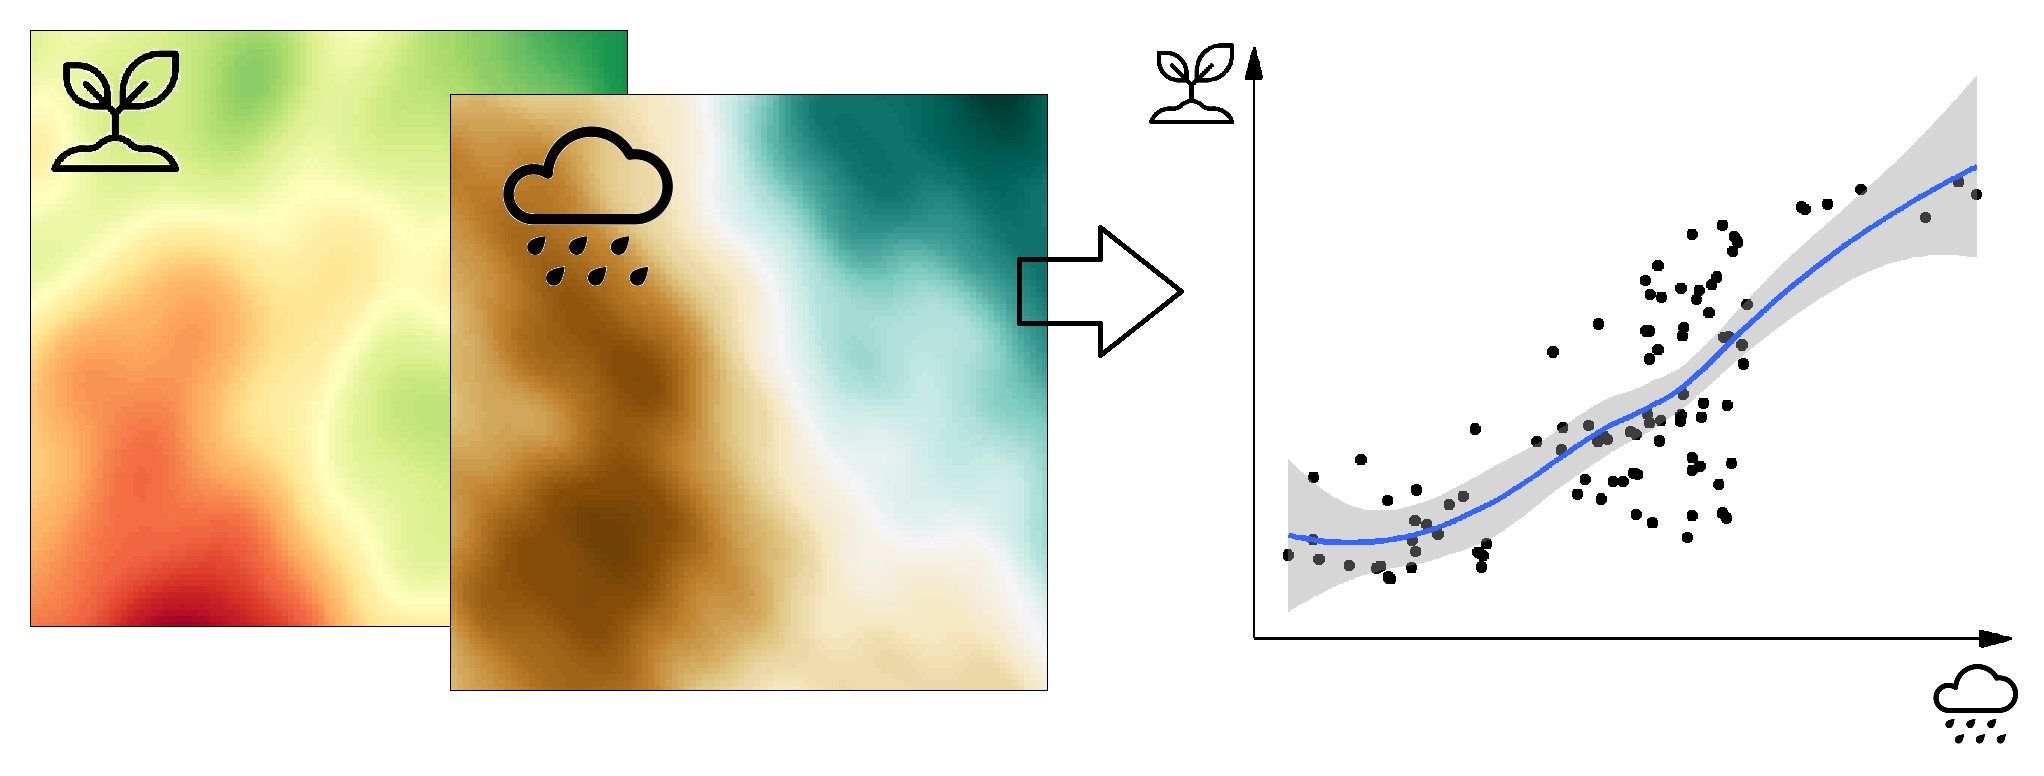
\includegraphics{species.png}

Possible explanations:

\begin{enumerate}
\tightlist
\item
  A direct causal effect
\item
  An indirect causal effect
\item
  An accidental spatial association
\end{enumerate}
\end{frame}

\hypertarget{chapman-2010}{%
\subsection{Chapman 2010}\label{chapman-2010}}

\begin{frame}{Chapman 2010}
\small


\includegraphics{chap_header.png}


\includegraphics[width=0.4\textwidth,height=\textheight]{picto_plants.jpg}

Data:

\begin{itemize}
\tightlist
\item
  100 UK plant species at 10x10 km grid
\item
  23 climatic variables
\item
  simulated variables with same properties
\end{itemize}

Models:

\begin{itemize}
\tightlist
\item
  GLM, random forests
\item
  non-spatial models, trend surfaces, autoregression
\item
  Single predictors, PCA
\end{itemize}
\end{frame}

\hypertarget{chapman-2010-1}{%
\subsection{Chapman 2010}\label{chapman-2010-1}}

\begin{frame}{Chapman 2010}
\small

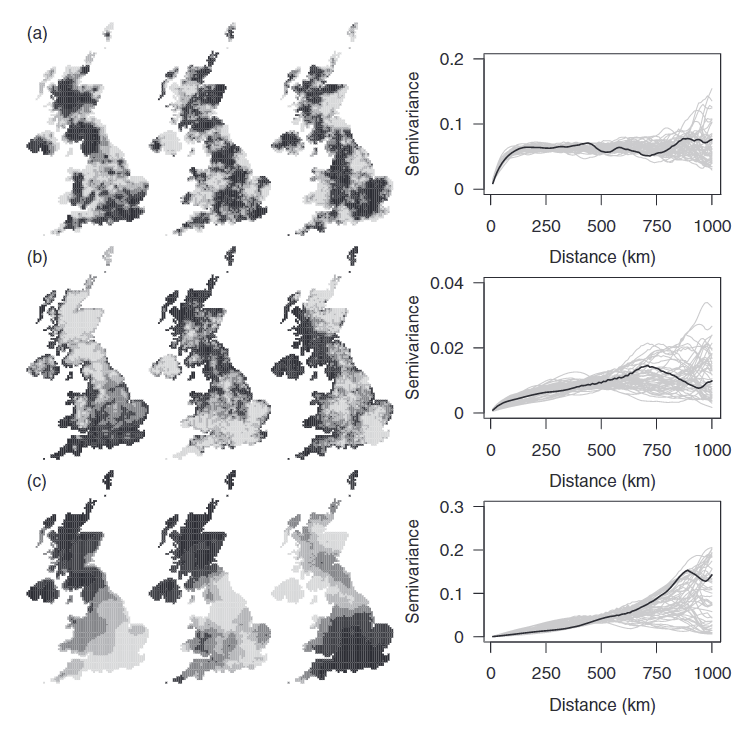
\includegraphics[width=\textwidth,height=0.9\textheight]{chap_sims.png}
\end{frame}

\hypertarget{chapman-2010-2}{%
\subsection{Chapman 2010}\label{chapman-2010-2}}

\begin{frame}{Chapman 2010}
\small

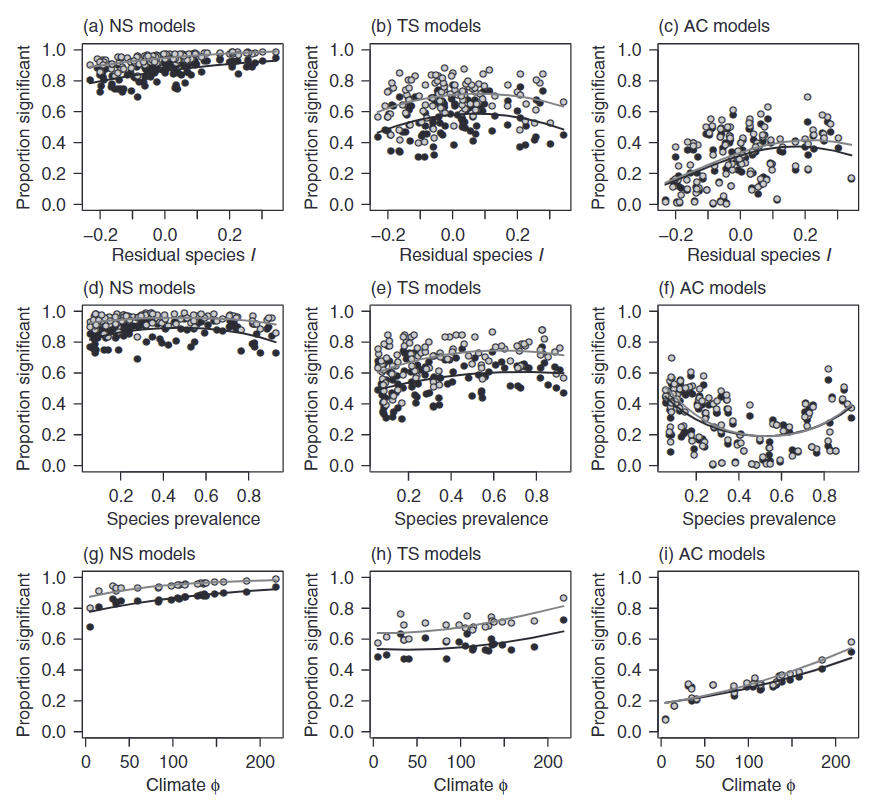
\includegraphics[width=\textwidth,height=0.9\textheight]{chap_single.png}
\end{frame}

\hypertarget{fourcade-besnard-secondi-2018}{%
\subsection{Fourcade, Besnard, Secondi
2018}\label{fourcade-besnard-secondi-2018}}

\begin{frame}{Fourcade, Besnard, Secondi 2018}
\small


\includegraphics[width=0.8\textwidth,height=\textheight]{paint_header.png}

\begin{itemize}
\tightlist
\item
  497 species from European Red List (GBIF)
\item
  real environmental predictors vs paintings
\end{itemize}

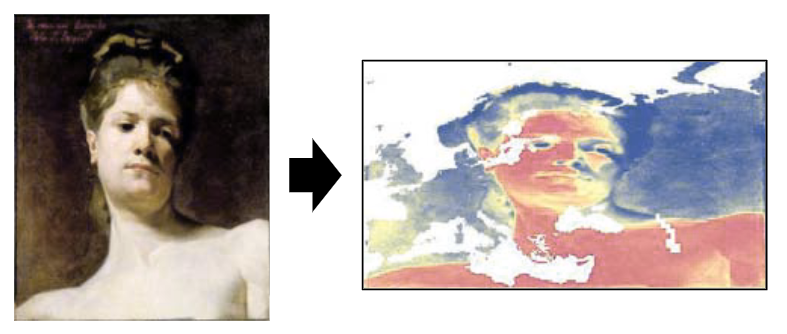
\includegraphics{paint_paint.png}
\end{frame}

\hypertarget{fourcade-besnard-secondi-2018-1}{%
\subsection{Fourcade, Besnard, Secondi
2018}\label{fourcade-besnard-secondi-2018-1}}

\begin{frame}{Fourcade, Besnard, Secondi 2018}
\small

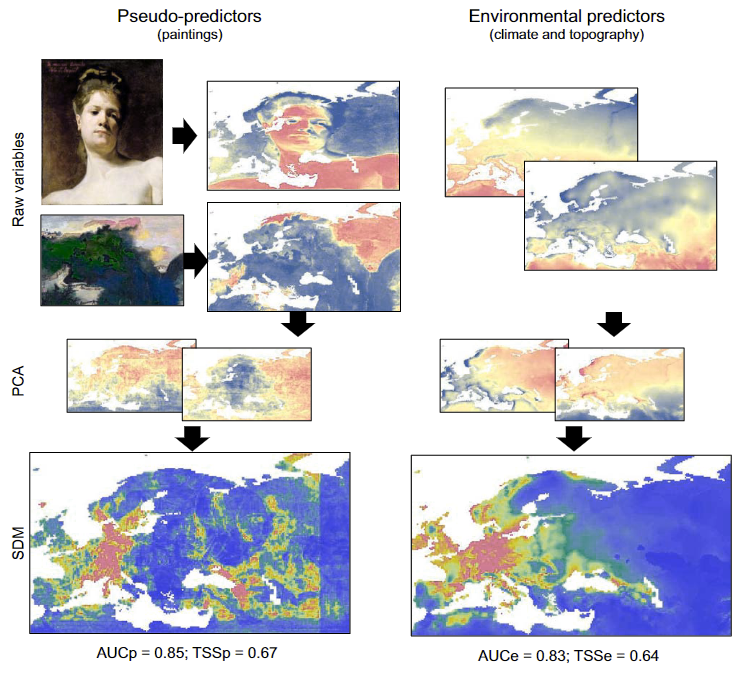
\includegraphics[width=\textwidth,height=0.9\textheight]{paint_scheme.png}
\end{frame}

\hypertarget{measuring-sac}{%
\section{Measuring SAC}\label{measuring-sac}}

\hypertarget{correlation-of-two-variables}{%
\subsection{Correlation of two
variables}\label{correlation-of-two-variables}}

\begin{frame}{Correlation of two variables}
\small

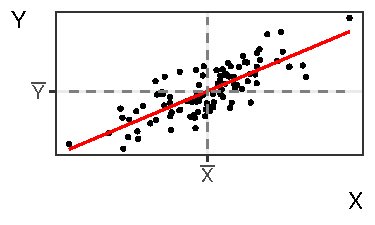
\includegraphics{Lecture_1_files/figure-beamer/unnamed-chunk-2-1.pdf}

Sample covariance:
\(S_{XY}=\frac{1}{n-1}\sum_{i=1}^n(X_i-\bar{X})(Y_i-\bar{Y})\)

Correlation coefficient: \(r=\frac{S_{XY}}{S_{X} S_{Y}}\),
\(-1 \le r \le 1\)

\(S_X\), \(S_Y\) \ldots{} sample standard deviations of \(X\), \(Y\)
\end{frame}

\hypertarget{correlation-of-two-variables-1}{%
\subsection{Correlation of two
variables}\label{correlation-of-two-variables-1}}

\begin{frame}{Correlation of two variables}
\small

\href{https://distill.pub/2019/visual-exploration-gaussian-processes/}{\textbf{Mathematical
model}}: \((X,Y) \sim MVN(\boldsymbol\mu, \boldsymbol\Sigma)\)

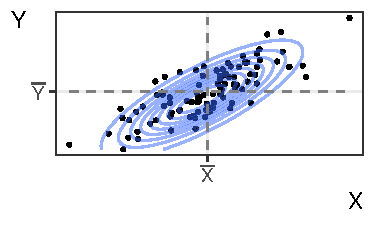
\includegraphics{Lecture_1_files/figure-beamer/unnamed-chunk-3-1.pdf}

Variance matrix:
\(\boldsymbol\Sigma=\begin{pmatrix}Var(X) & Cov(X,Y)\\Cov(X,Y) & Var(Y)\end{pmatrix}\)

Covariance: \(Cov(X,Y)=E[(X-E(X))(Y-E(Y))]\)

Correlation coefficient: \(\rho = \frac{Cov(X,Y)}{\sigma(X)\sigma(Y)}\)
\end{frame}

\hypertarget{spatial-autocorrelation}{%
\subsection{Spatial autocorrelation}\label{spatial-autocorrelation}}

\begin{frame}{Spatial autocorrelation}
\small

Point observations in space:

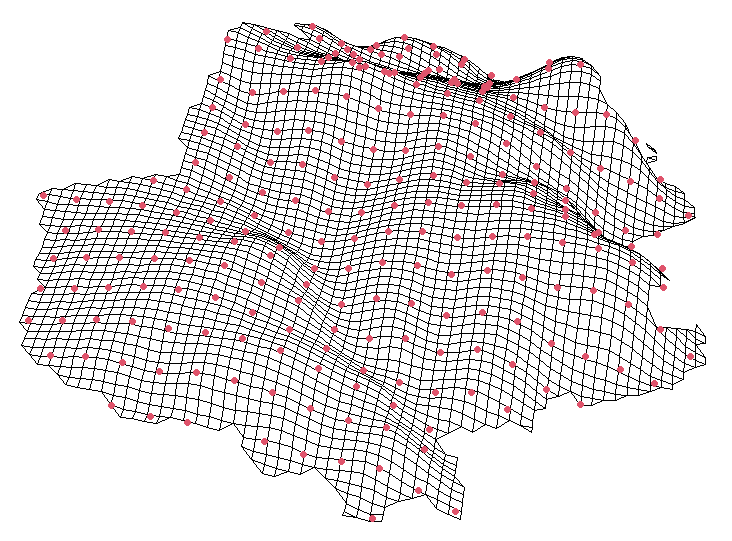
\includegraphics[width=10.17in,height=0.3\textheight]{terrain2}

::::\{.columns\} :::\{.column\}

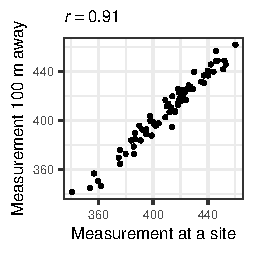
\includegraphics{Lecture_1_files/figure-beamer/unnamed-chunk-5-1.pdf}

::::
\end{frame}

\hypertarget{spatial-autocorrelation-1}{%
\subsection{Spatial autocorrelation}\label{spatial-autocorrelation-1}}

\begin{frame}{Spatial autocorrelation}
\small

Point observations in space:

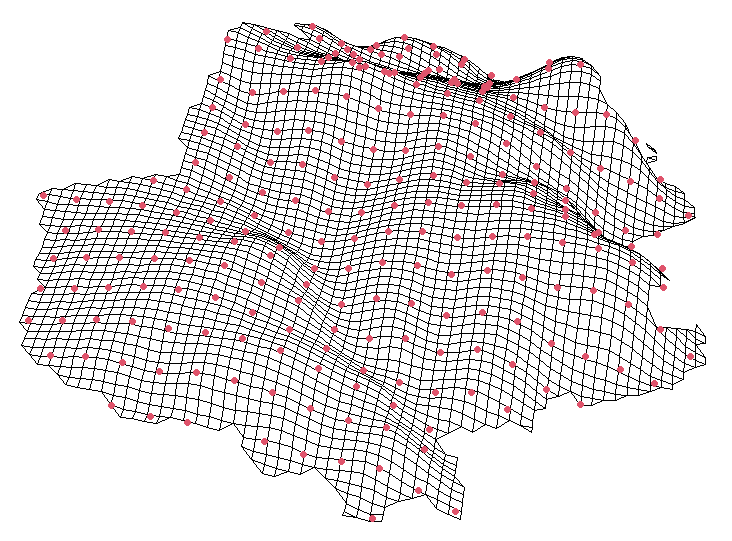
\includegraphics[width=10.17in,height=0.3\textheight]{terrain2}

Correlation as a function of distance (correlogram):

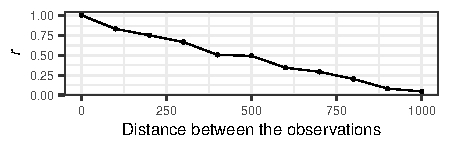
\includegraphics{Lecture_1_files/figure-beamer/unnamed-chunk-7-1.pdf}

\begin{itemize}
\tightlist
\item
  Assumption: the underlying spatial process is \textbf{stacionary} and
  \textbf{isotropic}!
\end{itemize}
\end{frame}

\hypertarget{morans-i}{%
\subsection{Moran's I}\label{morans-i}}

\begin{frame}{Moran's I}
\small

\[I=\frac{n}{\sum_{i=1}^n \sum_{i=1}^n w_{ij}} \frac{\sum_{i=1}^n \sum_{j=1}^n w_{ij} (y_i-\bar{y})(y_j-\bar{y})}{\sum_{i=1}^n(y_i-\bar{y})^2}\]

\begin{itemize}
\tightlist
\item
  \(w_{ij}\) measures the magnitude of spatial interactions between
  sites \(i\) and \(j\)
\item
  originally designed for lattice data!
\item
  Standard metric used for correlograms
\item
  Under the null hypothesis of spatial independence:
  \(E(I) = -1 / (n-1)\)
\item
  Alternative measure: Geary's C
\end{itemize}
\end{frame}

\hypertarget{local-morans-i}{%
\subsection{Local Moran's I}\label{local-morans-i}}

\begin{frame}{Local Moran's I}
\small

The (global) Moran's I can be decomposed into components assossiated
with the individual sites:

\[I_i = \frac{(y_i - \bar{y}) \sum_{j=1}^n w_{ij}(y_j-\bar{y})}{\frac{\sum_{j=1}^n(y_i-\bar{y})^2}{n}}\]

\[\sum_{i=1}^nI_i = I\]
\end{frame}

\hypertarget{correlogram}{%
\subsection{Correlogram}\label{correlogram}}

\hypertarget{gaussian-processes-correlation-function}{%
\section{Gaussian processes, correlation
function}\label{gaussian-processes-correlation-function}}

\hypertarget{gaussian-spatial-random-process}{%
\subsection{Gaussian (spatial random)
process}\label{gaussian-spatial-random-process}}

\begin{frame}{Gaussian (spatial random) process}
\small

\textbf{Gaussian process}: \(\left\{S(x):x\in \mathbb{R}^2\right\}\)

For any \(x_1,x_2,...,x_n\) -\textgreater{}
\(\left\{S(x_1),S(x_2),...,S(x_3)\right\}\sim MVN(\boldsymbol\mu, \boldsymbol\Sigma)\)

\begin{itemize}
\item
  \(\mu(x) = E\left[S(x)\right]\) \ldots{} mean function
\item
  \(C(x,x')=Cov\left(S(x),S(x')\right)\) \ldots{} covariance function
\end{itemize}

\emph{Stationary, isotropic process}: \(\mu(x)=\mu\), \(C(x,x')=C(u)\)

We can then define:

\begin{itemize}
\tightlist
\item
  \(\sigma^2=C(0)\) \ldots{} (constant) variance of the process
\end{itemize}

\begin{itemize}
\tightlist
\item
  \(\rho(u)=C(u)/\sigma^2\) \ldots{} \textbf{correlation function} of
  the process
\end{itemize}
\end{frame}

\hypertarget{power-exponential-family}{%
\subsection{Power-Exponential family}\label{power-exponential-family}}

\begin{frame}{Power-Exponential family}
\large

\[\rho(u)=exp\left\{-\left(\frac{u}{\phi}\right)^\kappa\right\}\]

\small

\(\phi\) \ldots{} scale, \(\phi>0\)

\(\kappa\) \ldots{} shape, \(0<\kappa\le 2\)

\begin{columns}[T]
\begin{column}{0.5\textwidth}
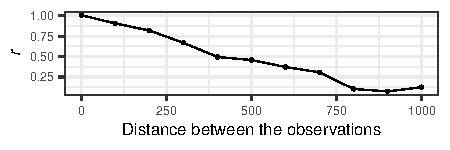
\includegraphics{Lecture_1_files/figure-beamer/unnamed-chunk-8-1.pdf}
\end{column}

\begin{column}{0.5\textwidth}
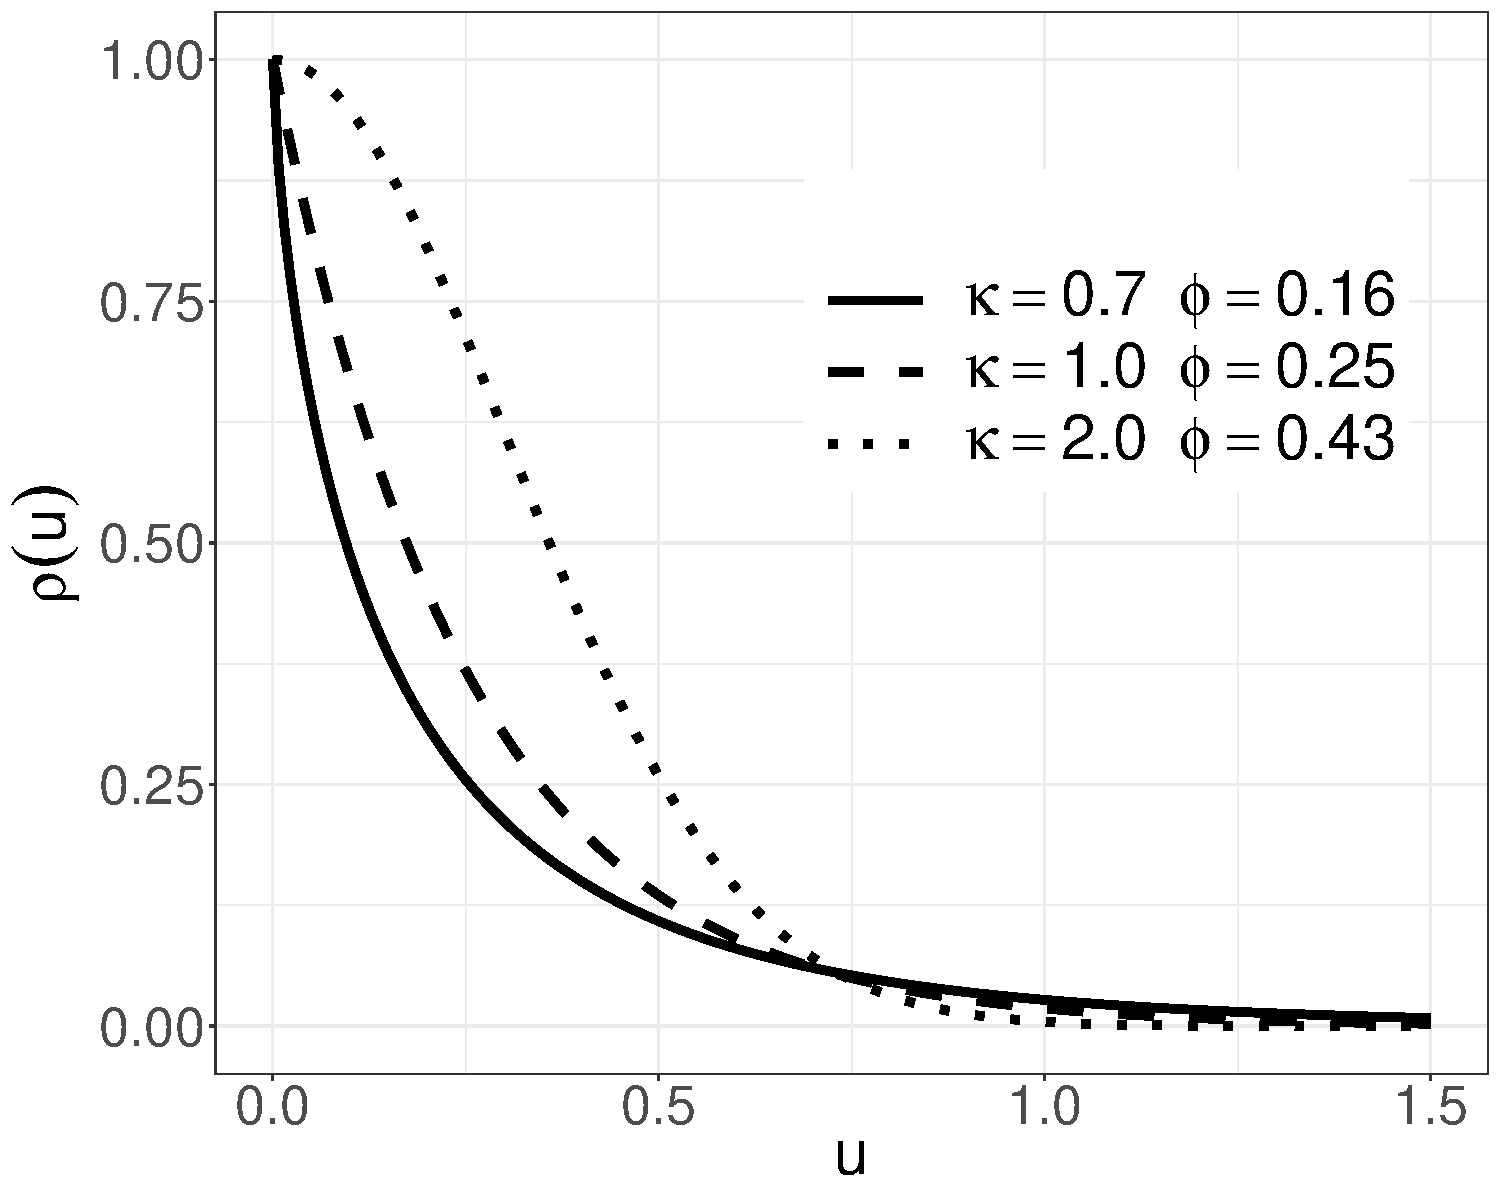
\includegraphics{Lecture_1_files/figure-beamer/unnamed-chunk-9-1.pdf}
\end{column}
\end{columns}
\end{frame}

\hypertarget{power-exponential-family-1}{%
\subsection{Power-Exponential family}\label{power-exponential-family-1}}

\begin{frame}{Power-Exponential family}
\large

\[\rho(u)=exp\left\{-\left(\frac{u}{\phi}\right)^\kappa\right\}\]

\small

\(\phi\) \ldots{} scale, \(\phi>0\)

\(\kappa\) \ldots{} shape, \(0<\kappa\le 2\)

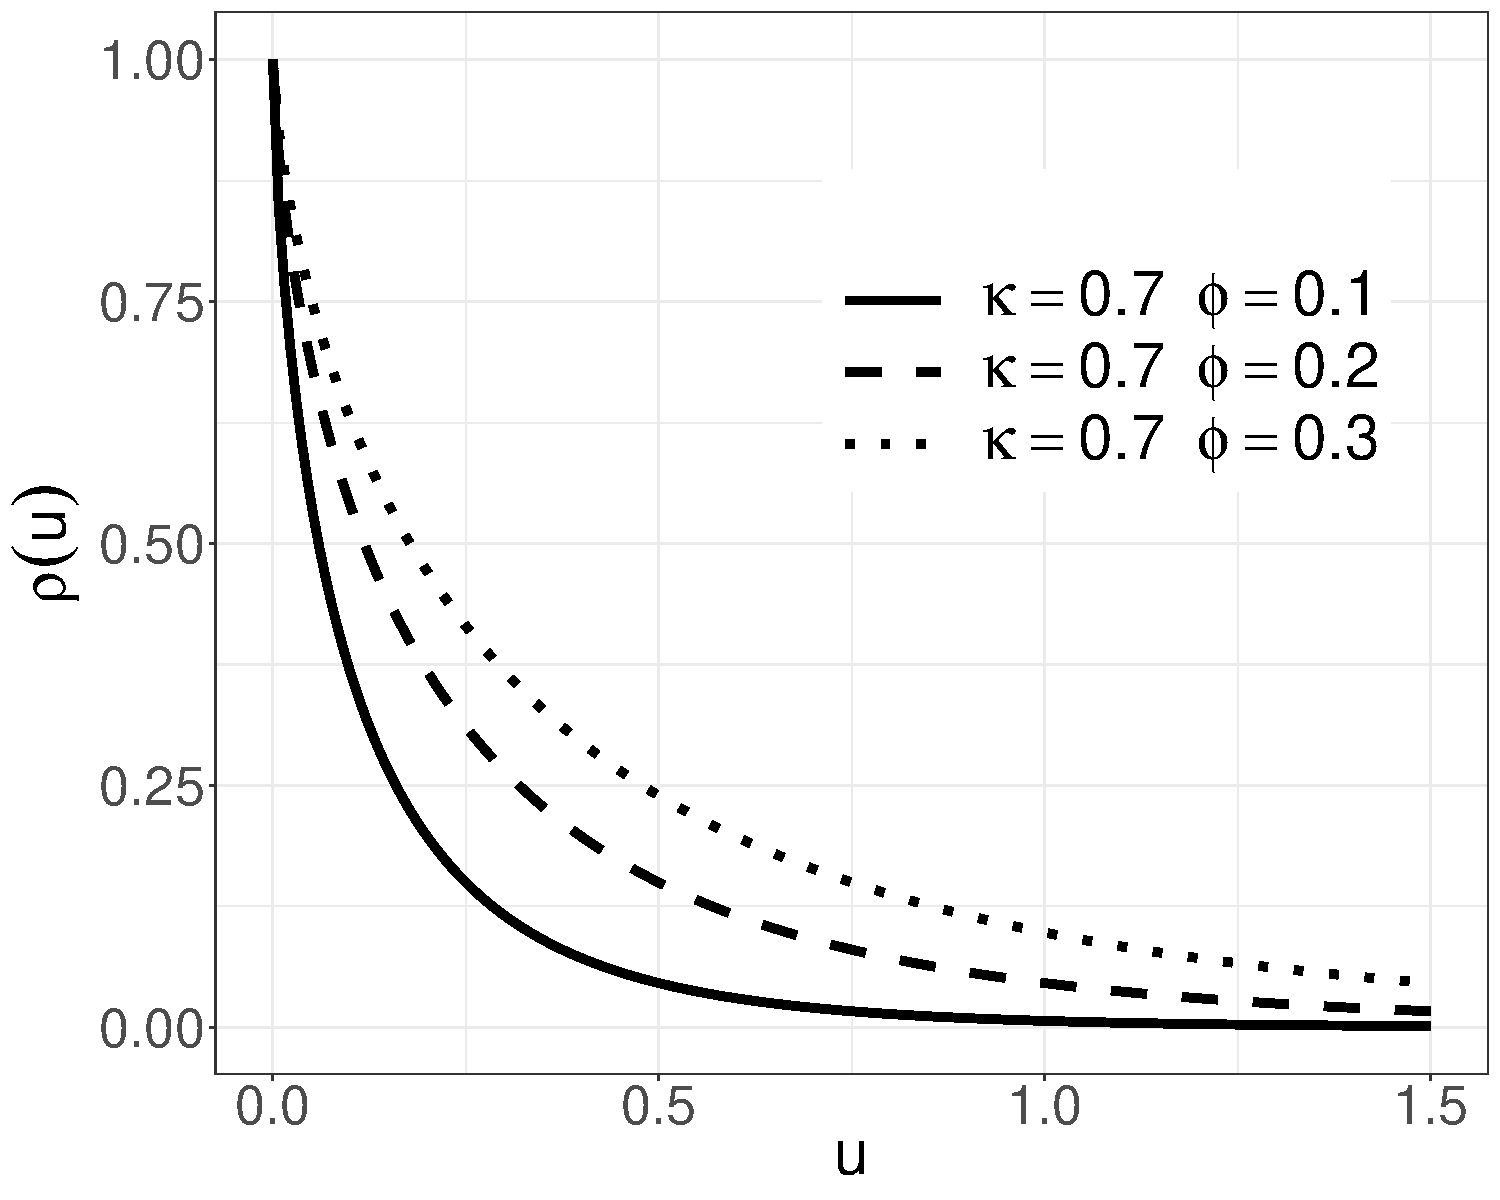
\includegraphics{Lecture_1_files/figure-beamer/unnamed-chunk-10-1.pdf}
\end{frame}

\hypertarget{power-exponential-family-2}{%
\subsection{Power-Exponential family}\label{power-exponential-family-2}}

\begin{frame}{Power-Exponential family}
\small

\begin{columns}[T]
\begin{column}{0.33\textwidth}
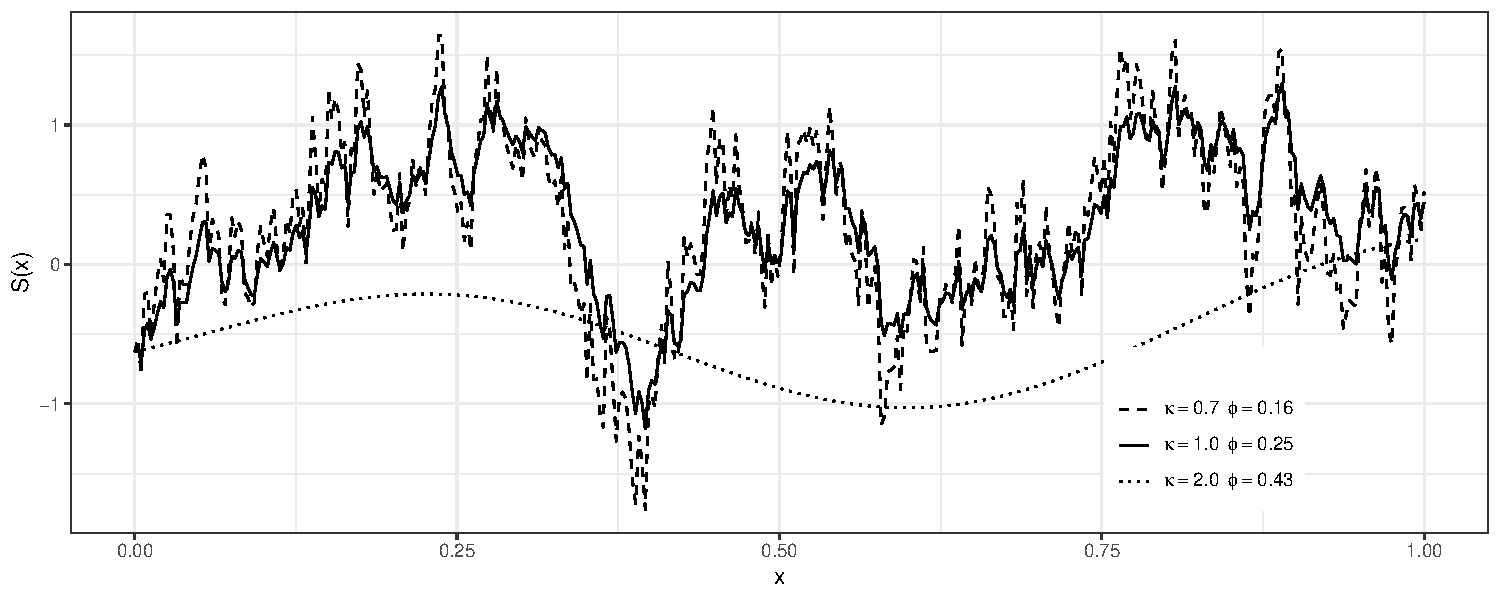
\includegraphics{Lecture_1_files/figure-beamer/unnamed-chunk-11-1.pdf}
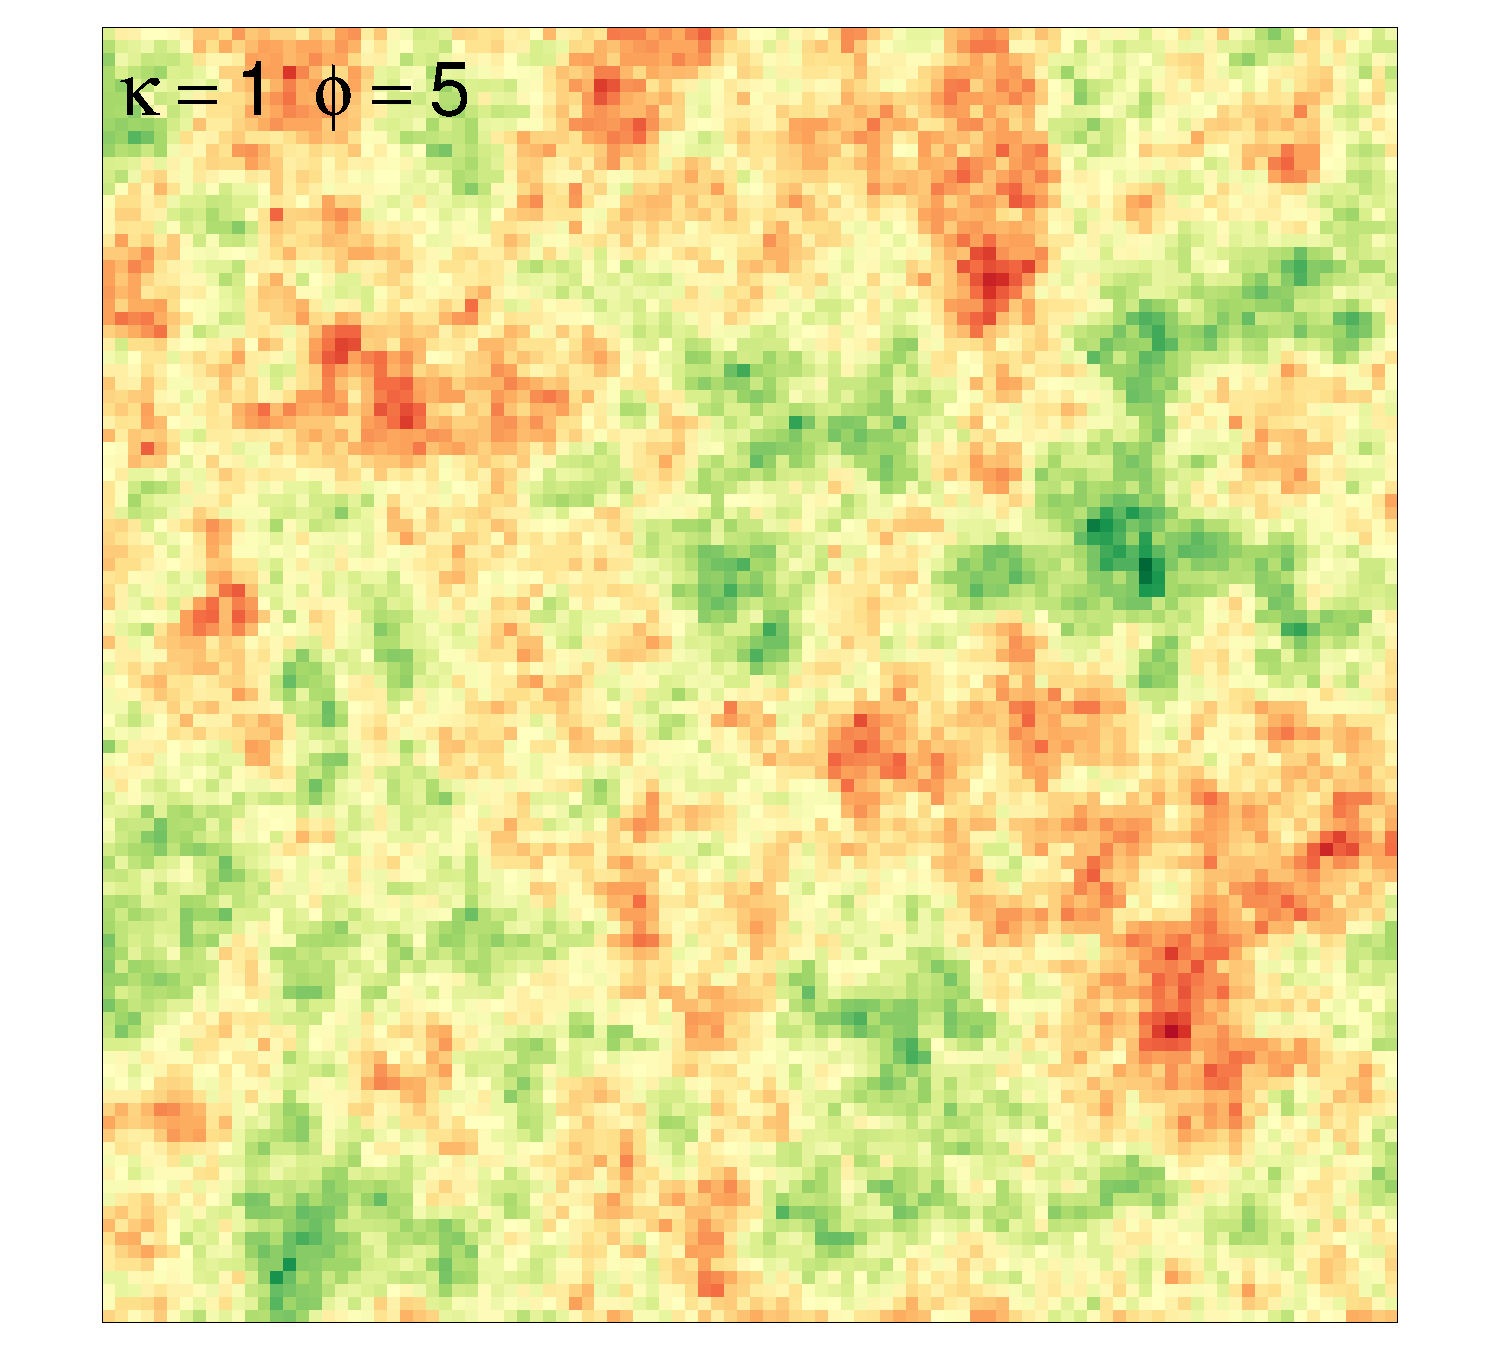
\includegraphics{Lecture_1_files/figure-beamer/unnamed-chunk-12-1.pdf}
\end{column}

\begin{column}{0.33\textwidth}
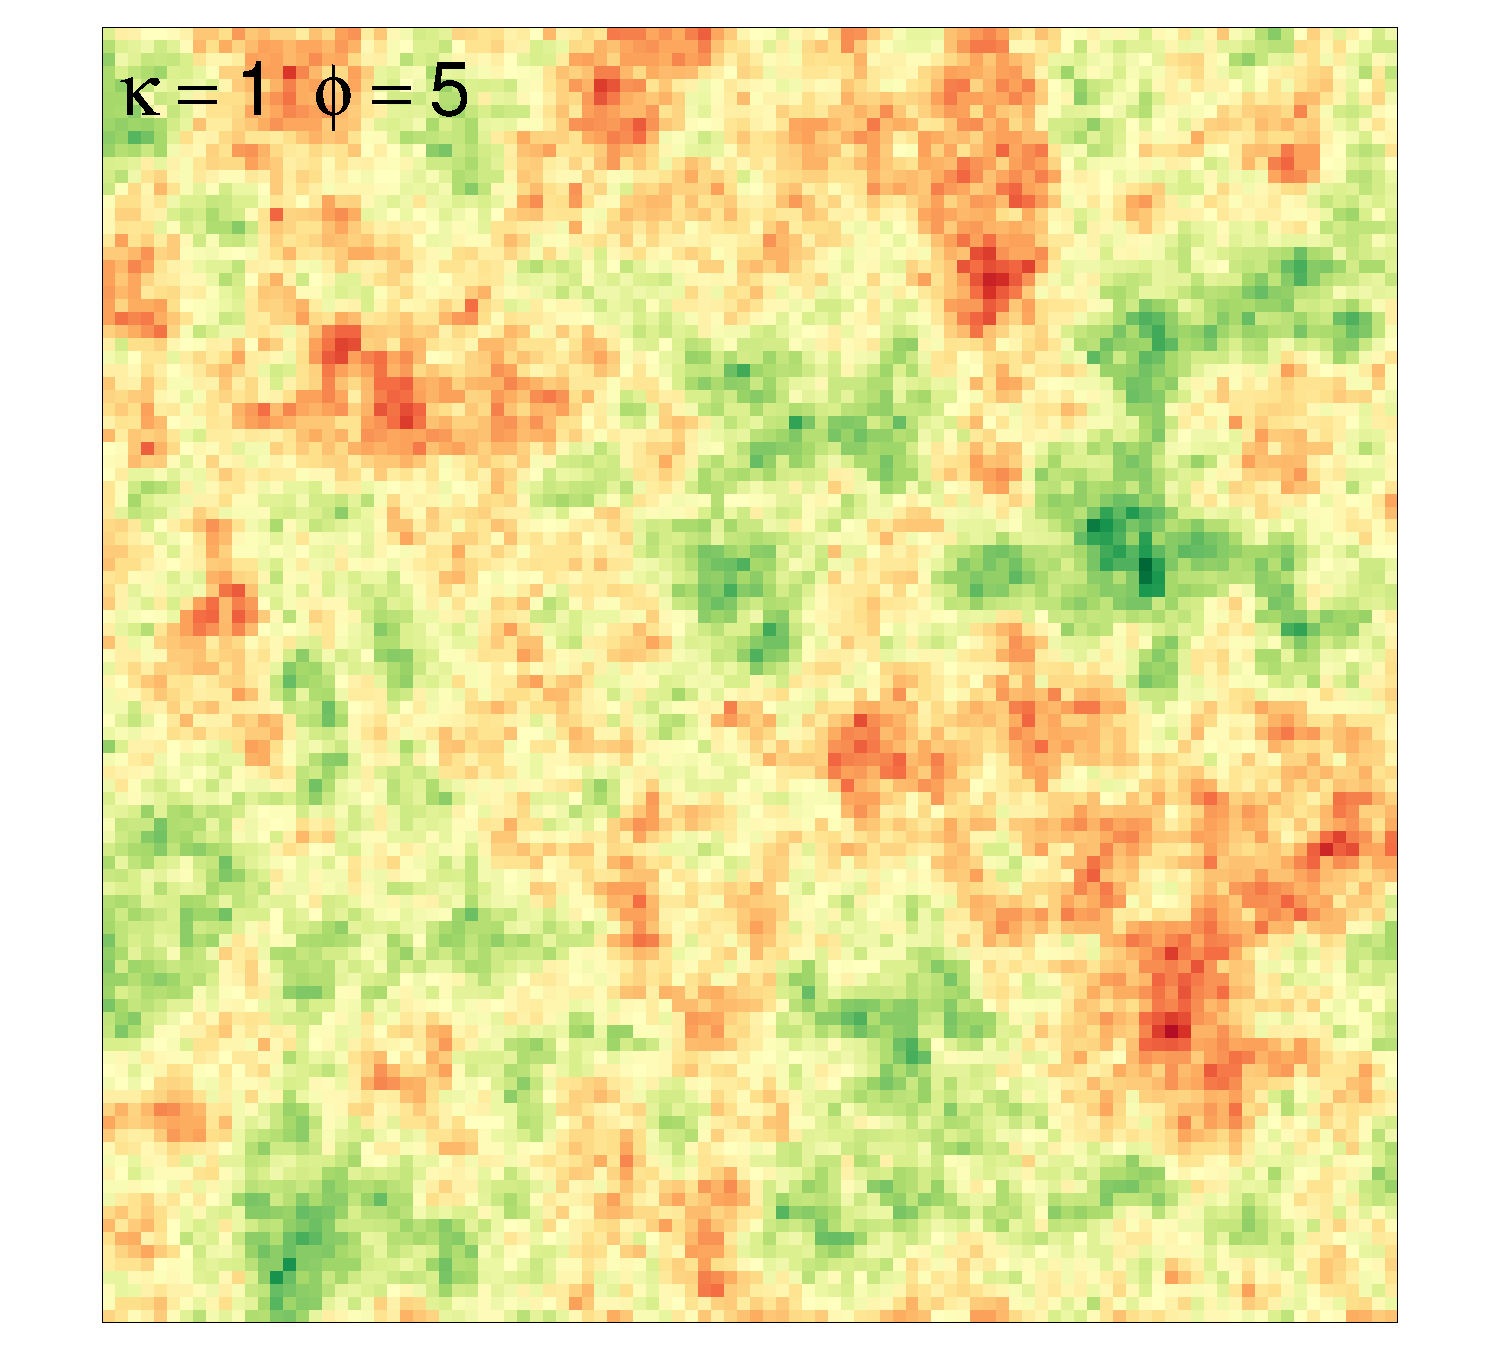
\includegraphics{Lecture_1_files/figure-beamer/unnamed-chunk-13-1.pdf}

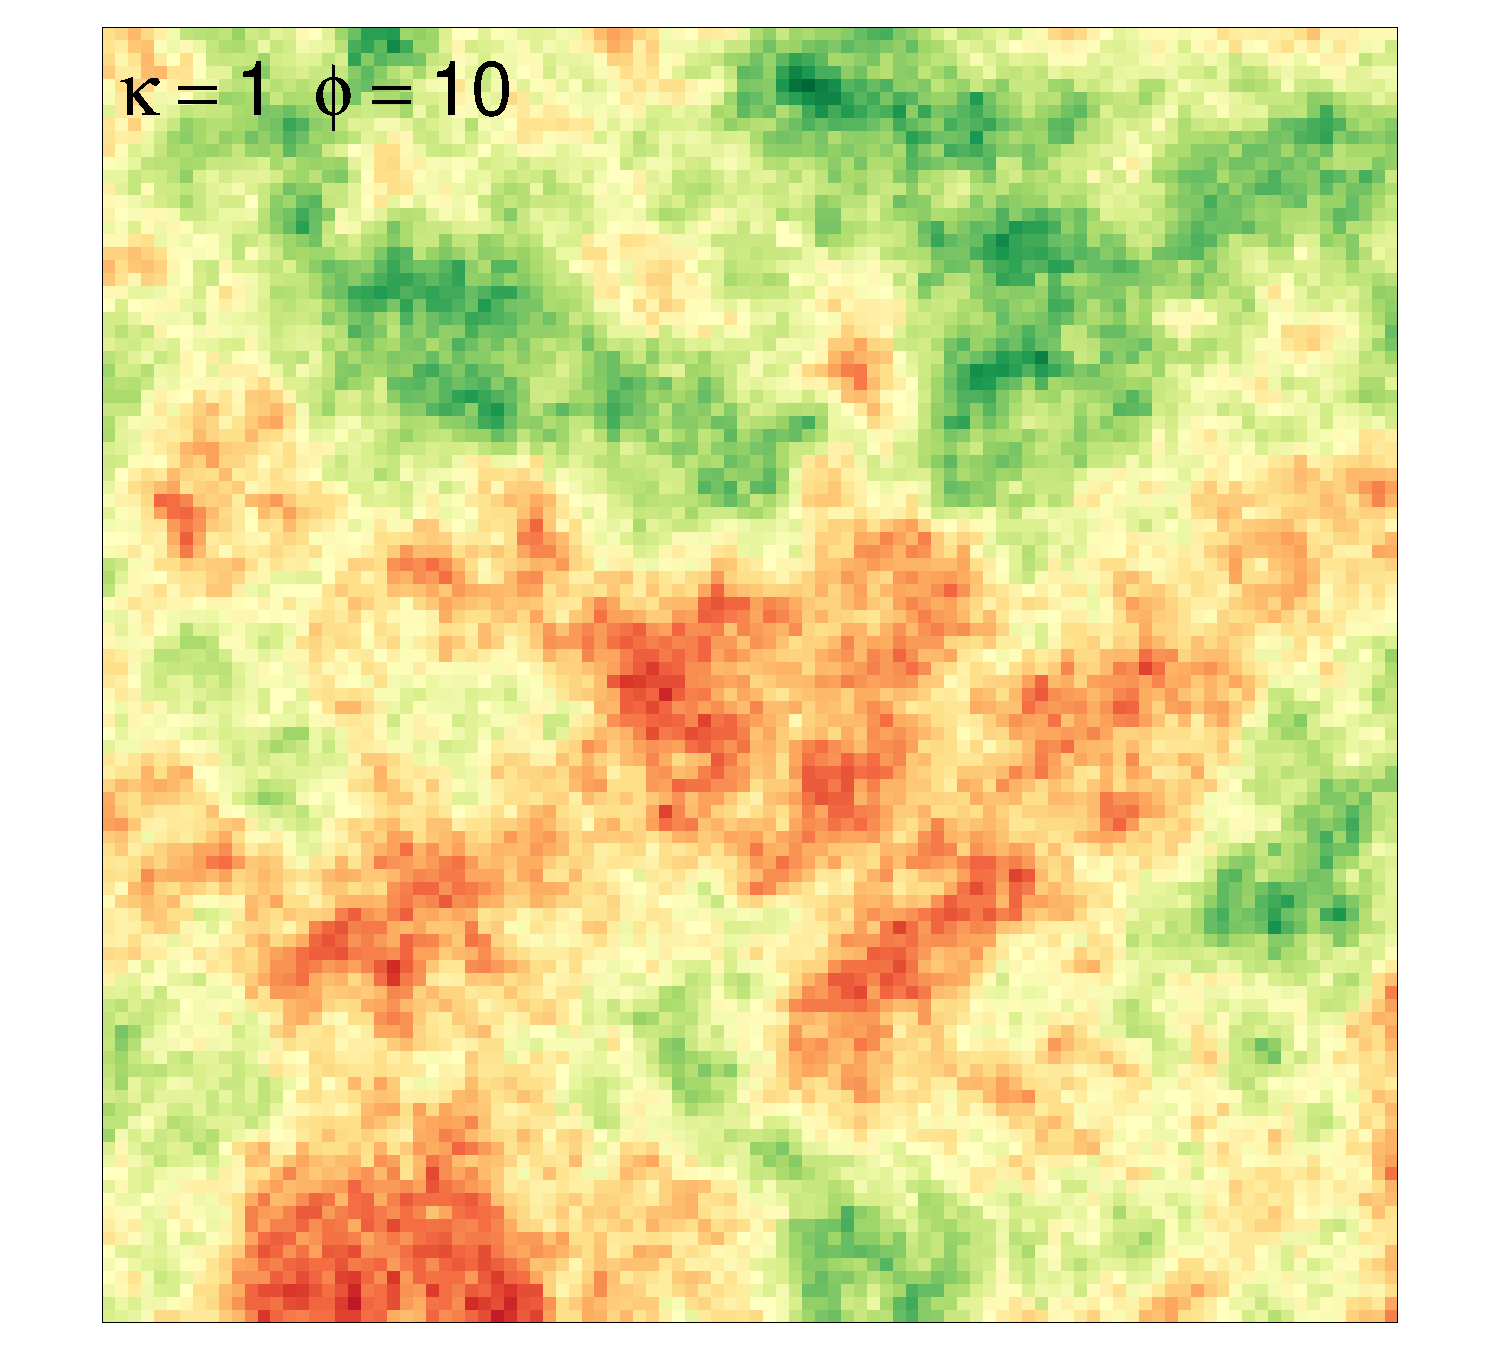
\includegraphics{Lecture_1_files/figure-beamer/unnamed-chunk-14-1.pdf}
\end{column}

\begin{column}{0.33\textwidth}
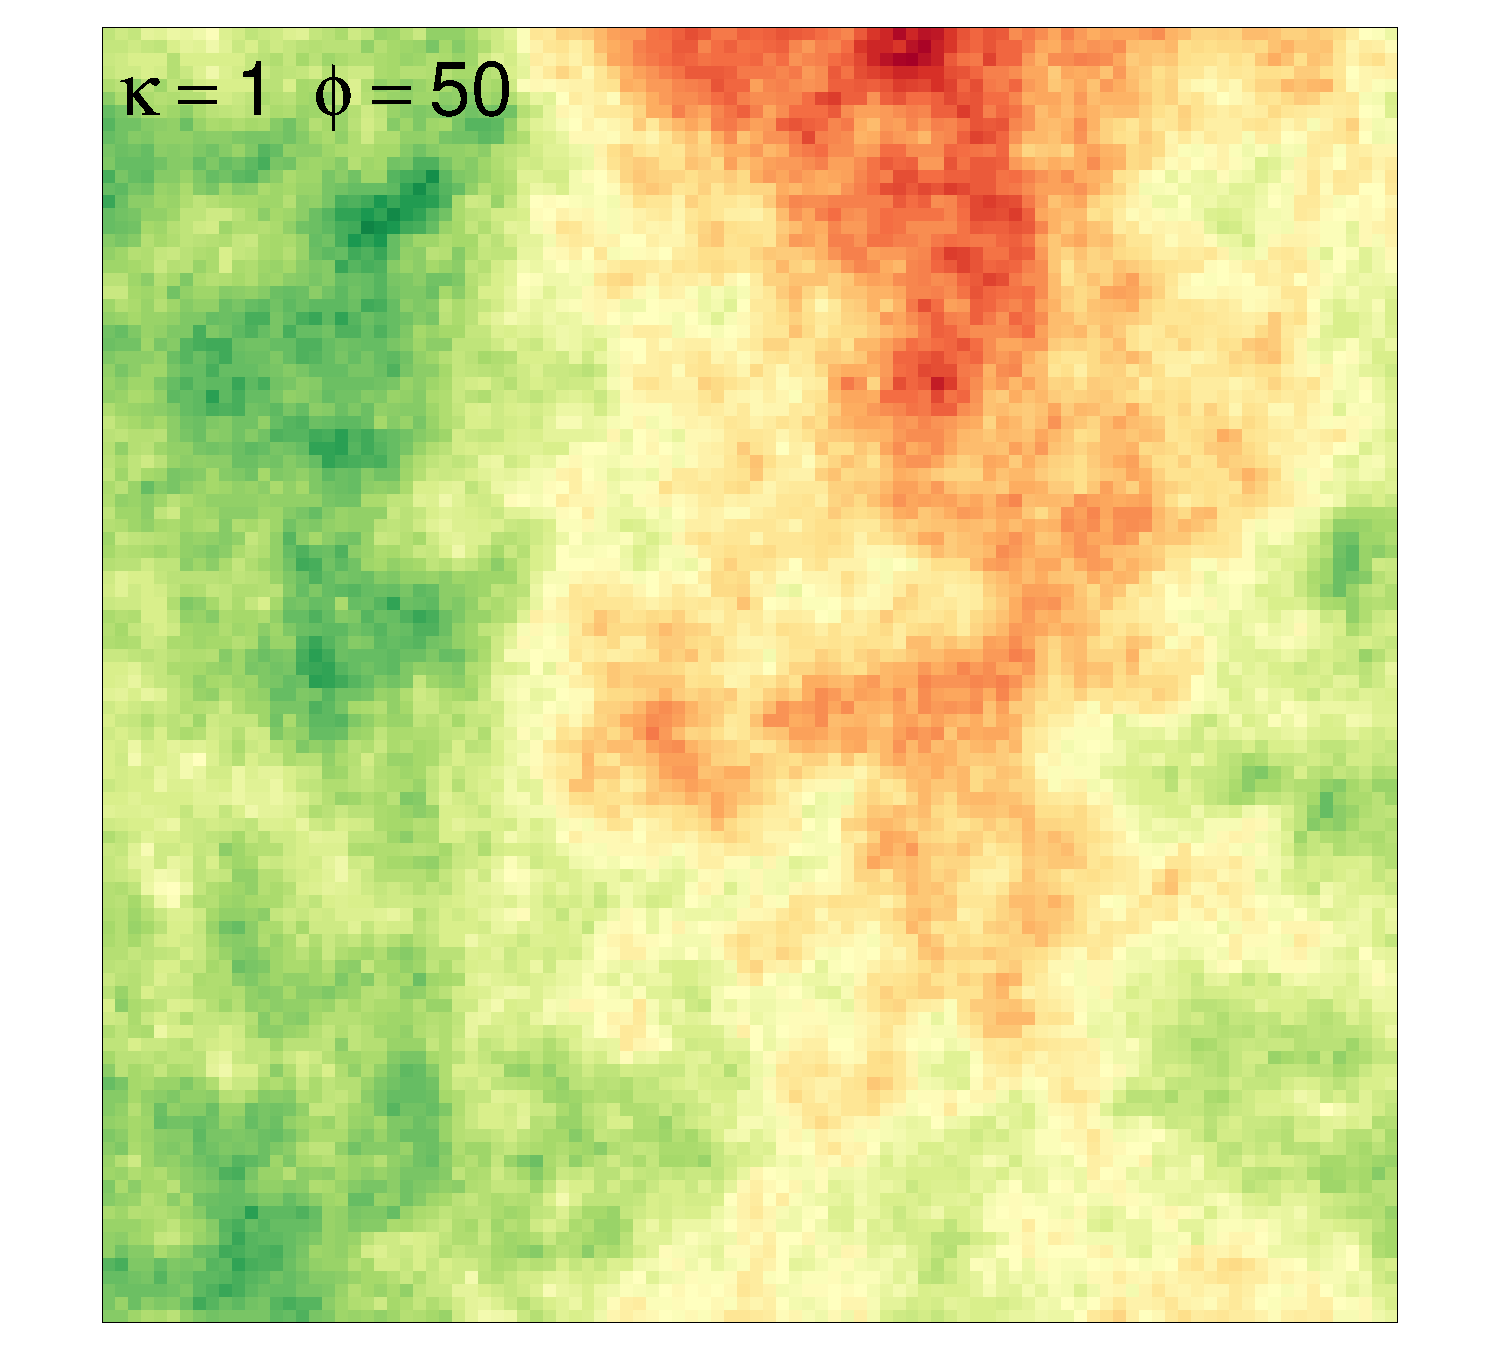
\includegraphics{Lecture_1_files/figure-beamer/unnamed-chunk-15-1.pdf}

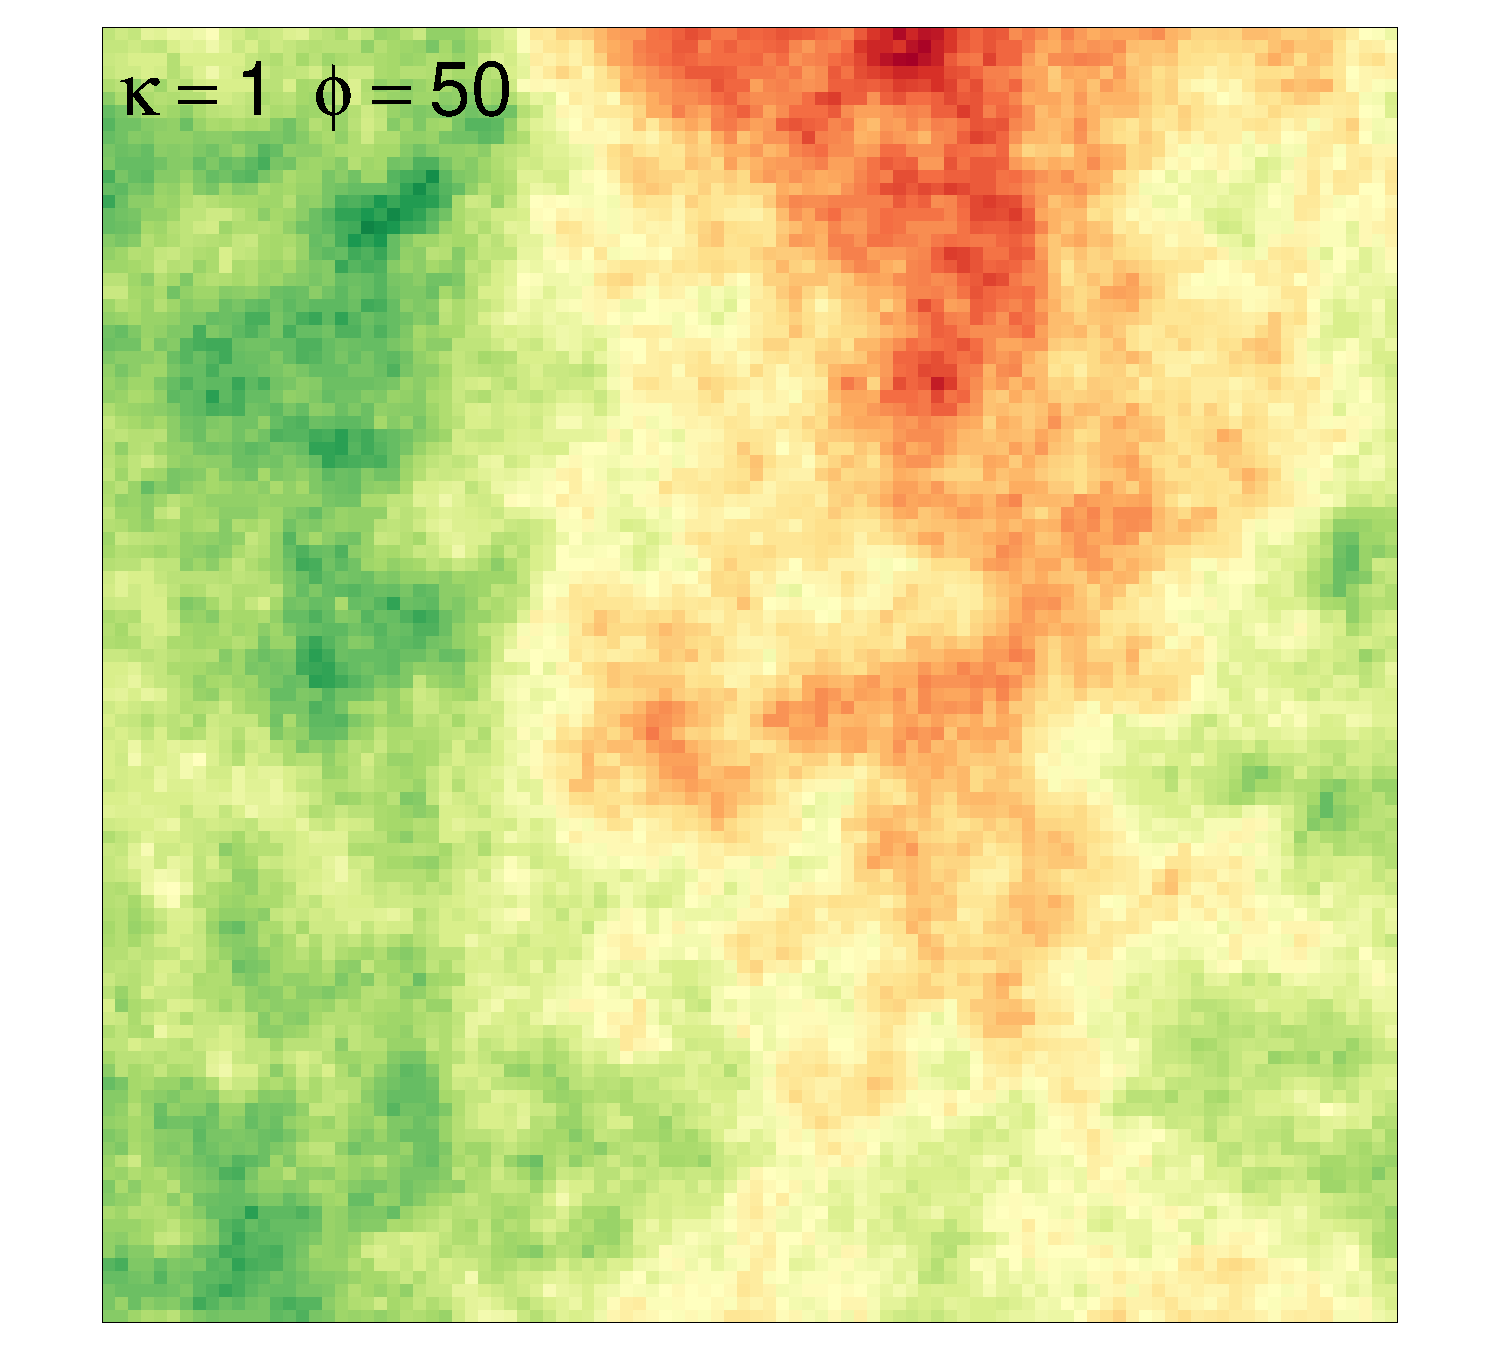
\includegraphics{Lecture_1_files/figure-beamer/unnamed-chunk-16-1.pdf}
\end{column}
\end{columns}
\end{frame}

\hypertarget{power-exponential-family-3}{%
\subsection{Power-Exponential family}\label{power-exponential-family-3}}

\begin{frame}{Power-Exponential family}
\small

\begin{columns}[T]
\begin{column}{0.33\textwidth}
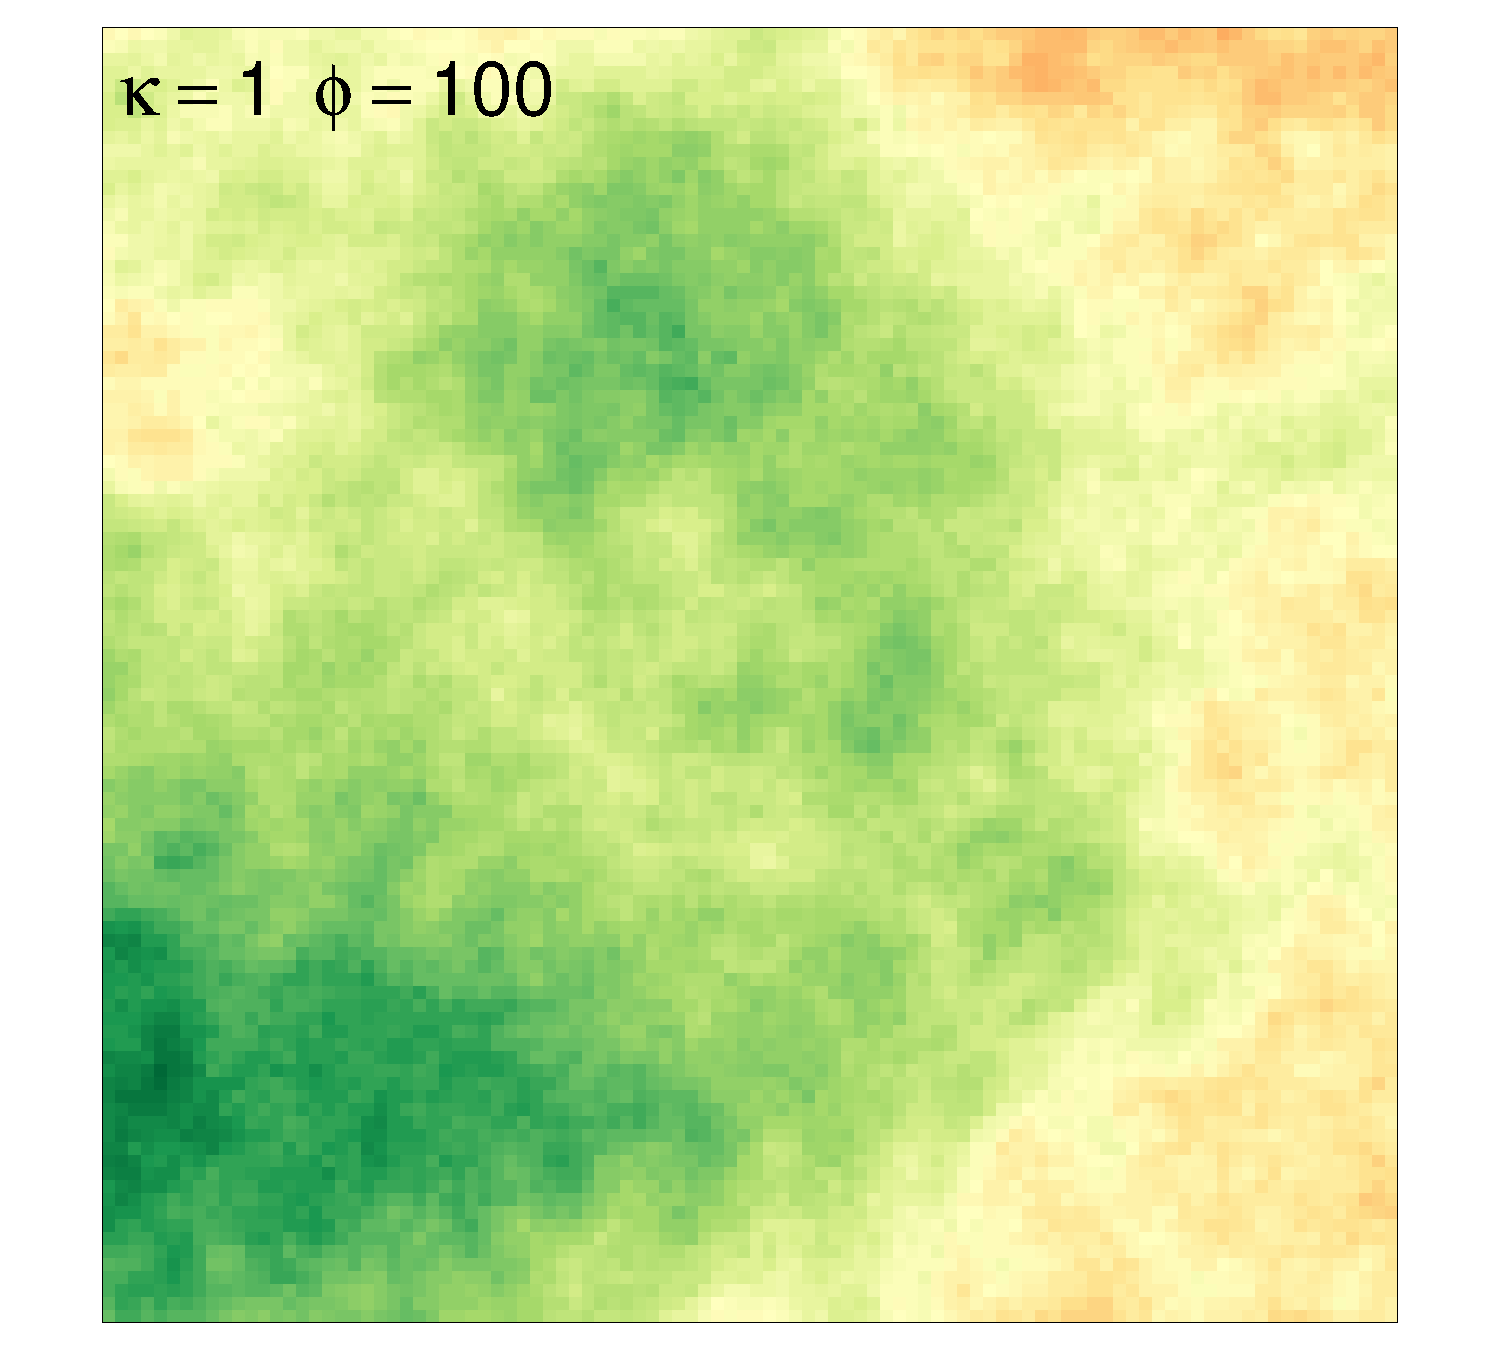
\includegraphics{Lecture_1_files/figure-beamer/unnamed-chunk-17-1.pdf}
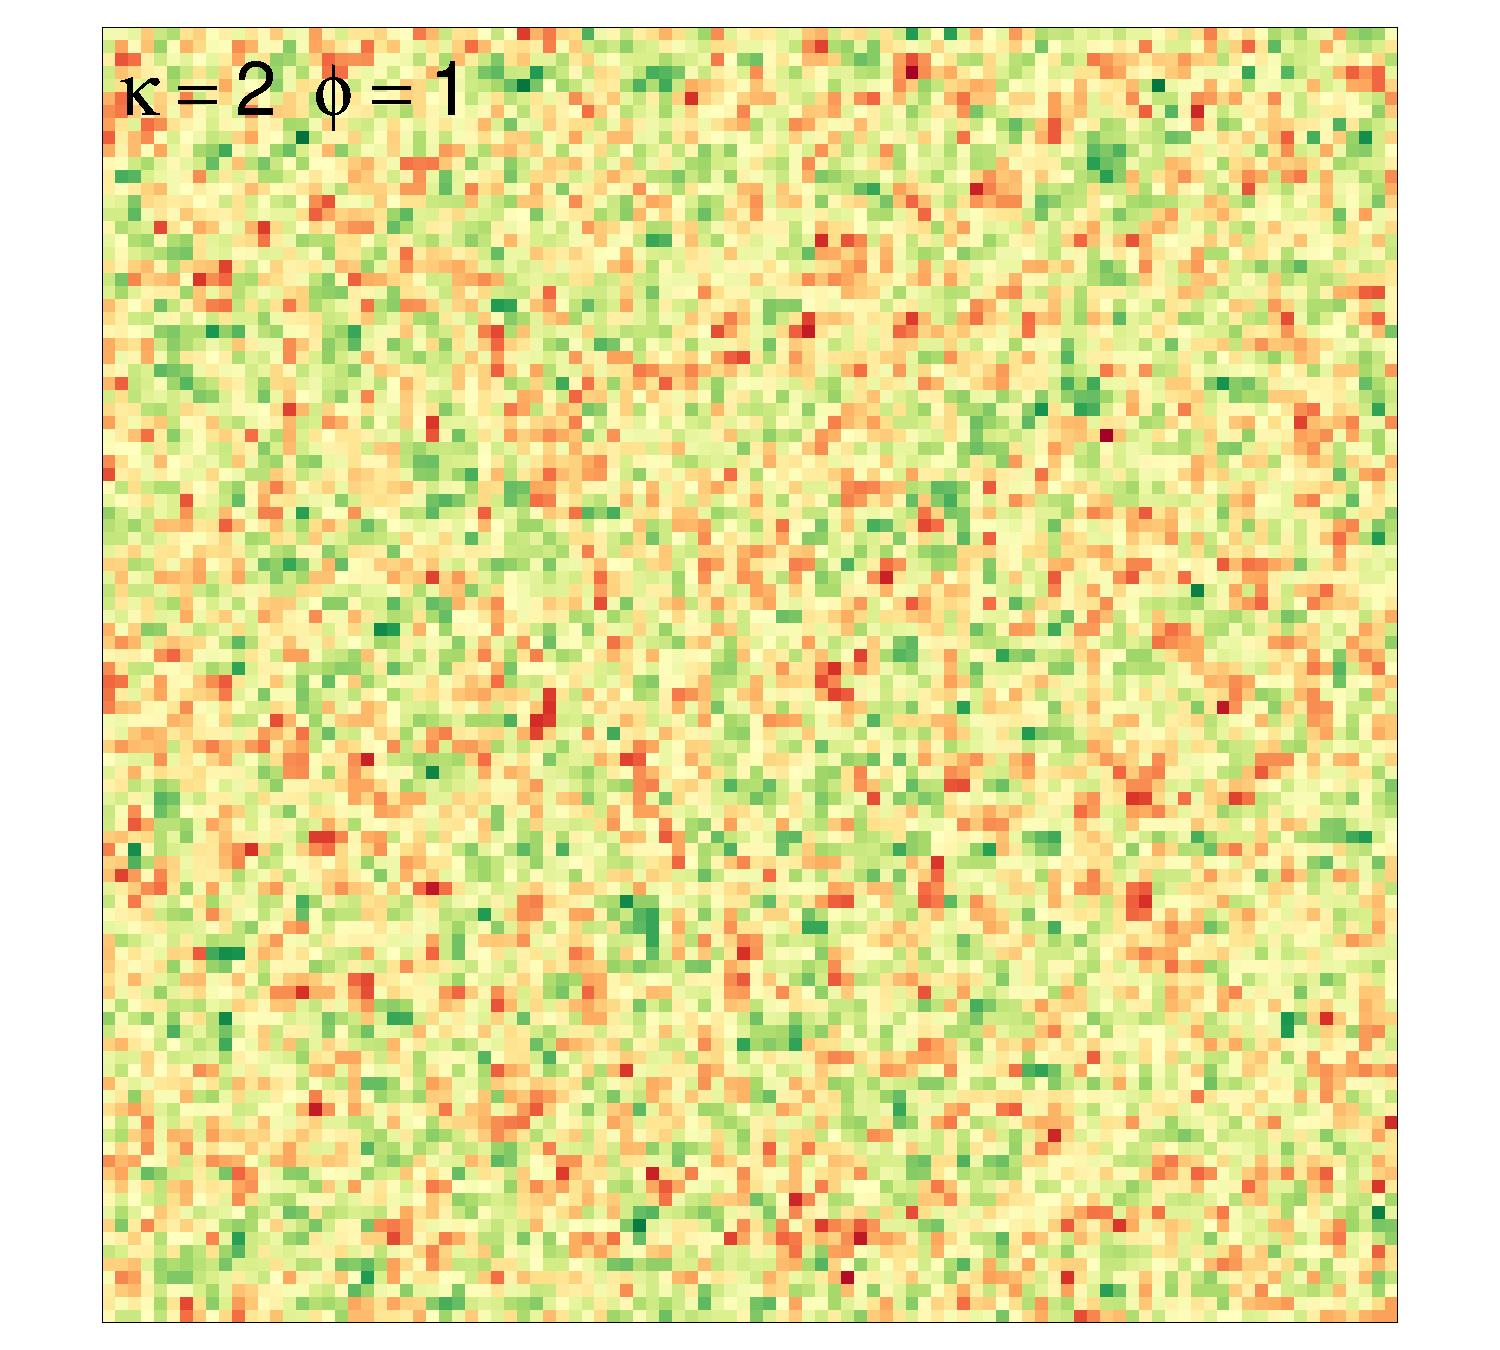
\includegraphics{Lecture_1_files/figure-beamer/unnamed-chunk-18-1.pdf}
\end{column}

\begin{column}{0.33\textwidth}
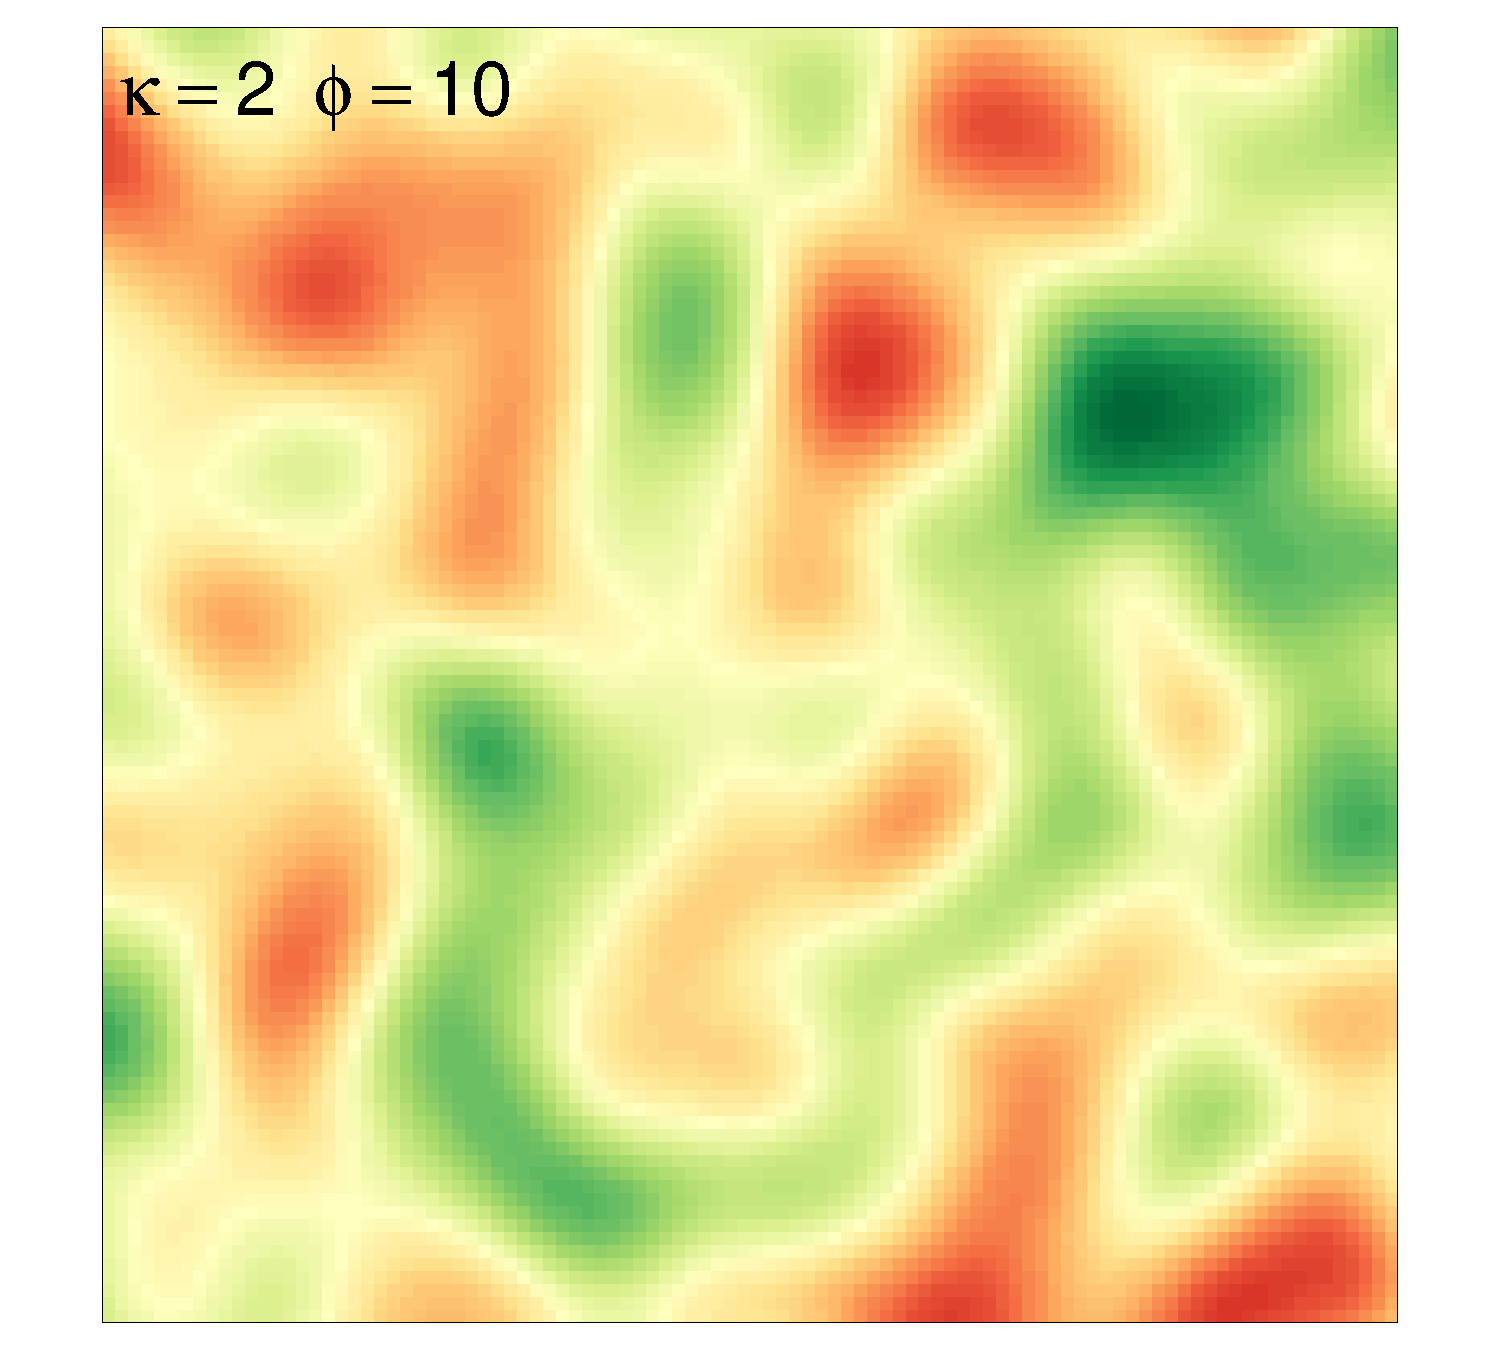
\includegraphics{Lecture_1_files/figure-beamer/unnamed-chunk-19-1.pdf}

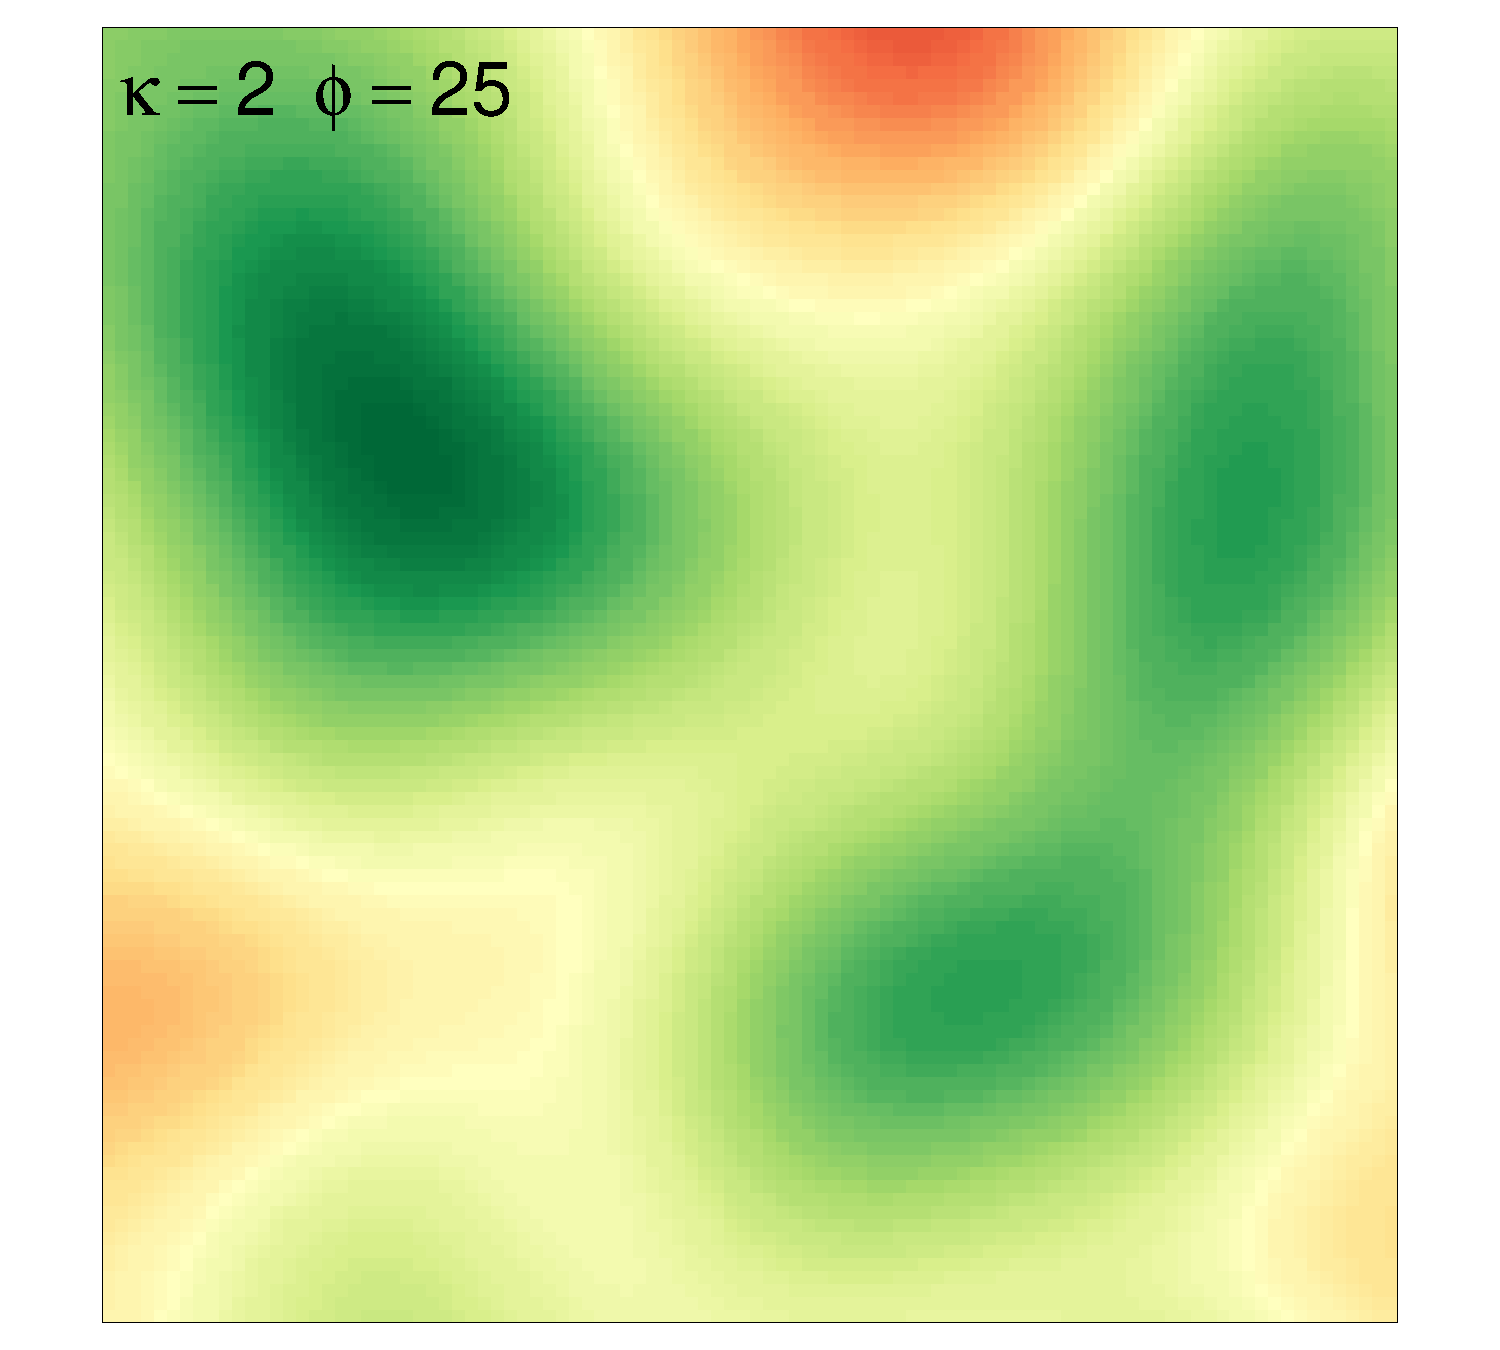
\includegraphics{Lecture_1_files/figure-beamer/unnamed-chunk-20-1.pdf}
\end{column}

\begin{column}{0.33\textwidth}
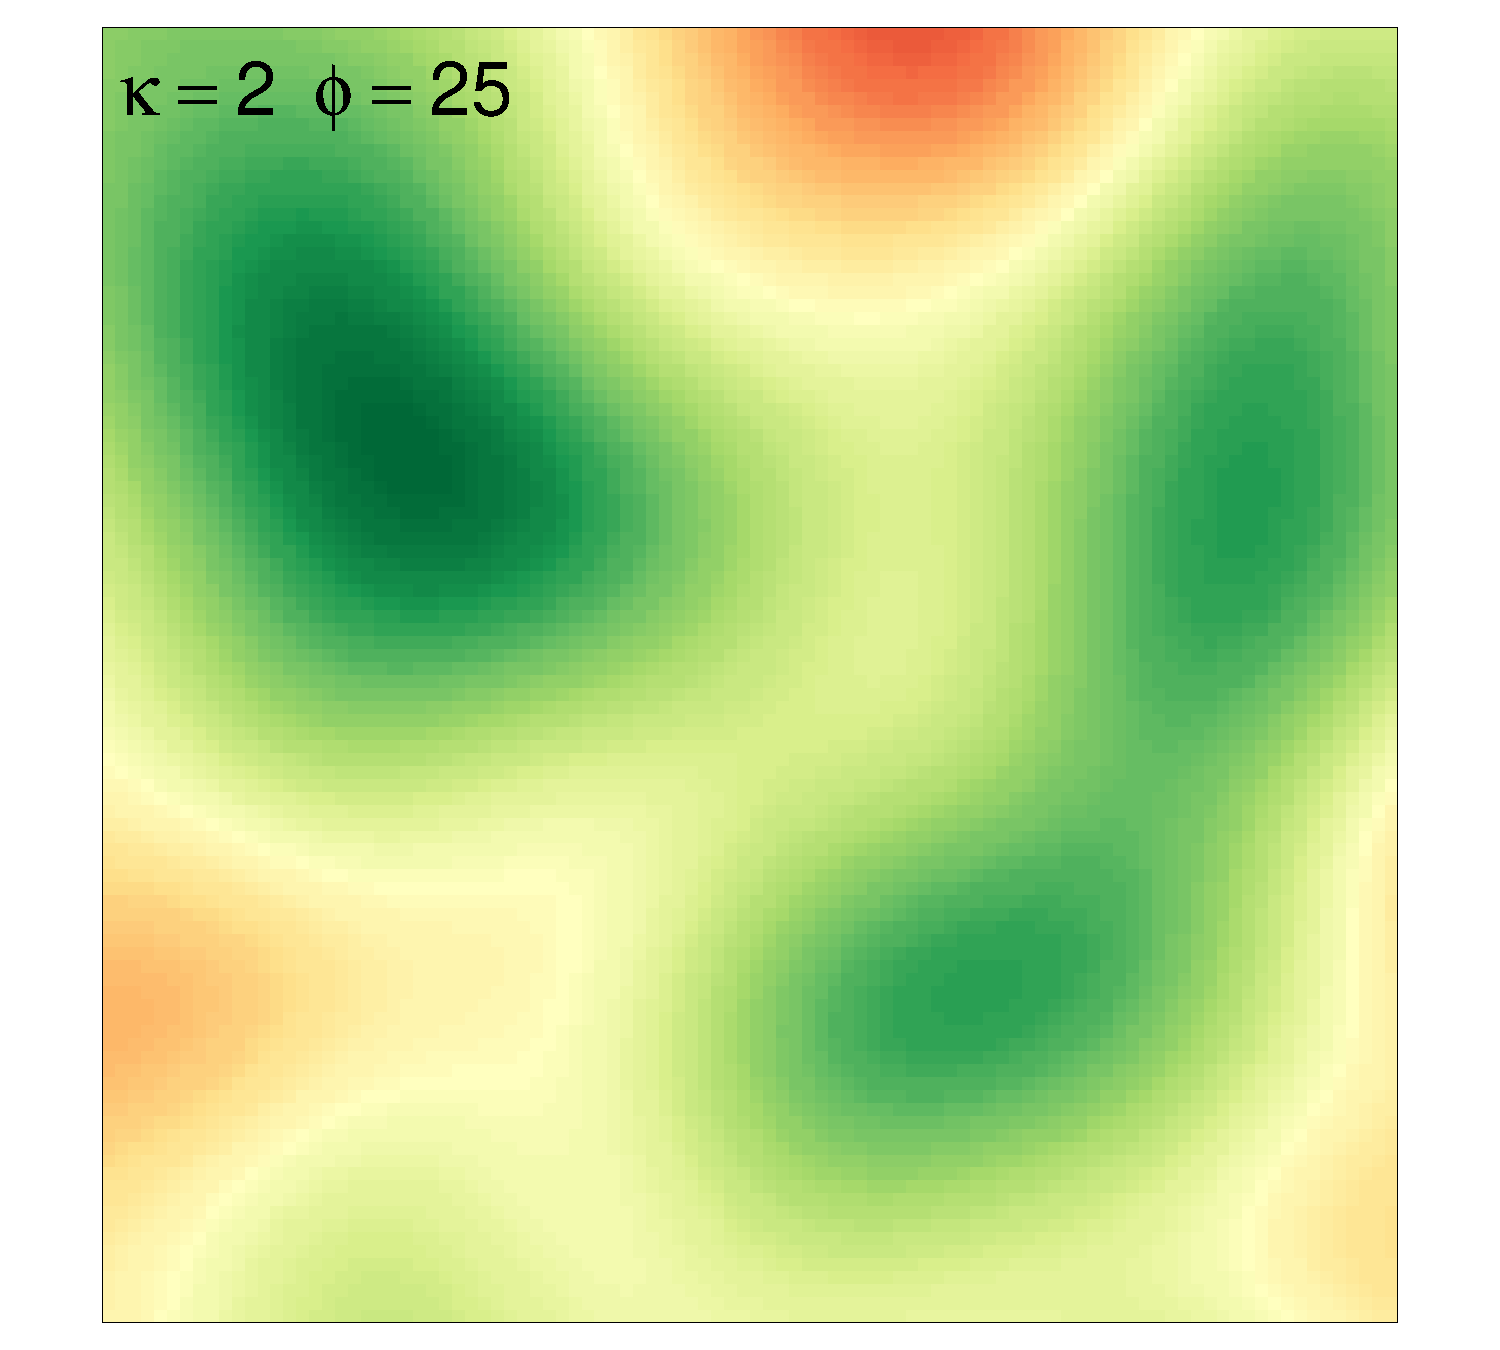
\includegraphics{Lecture_1_files/figure-beamer/unnamed-chunk-21-1.pdf}

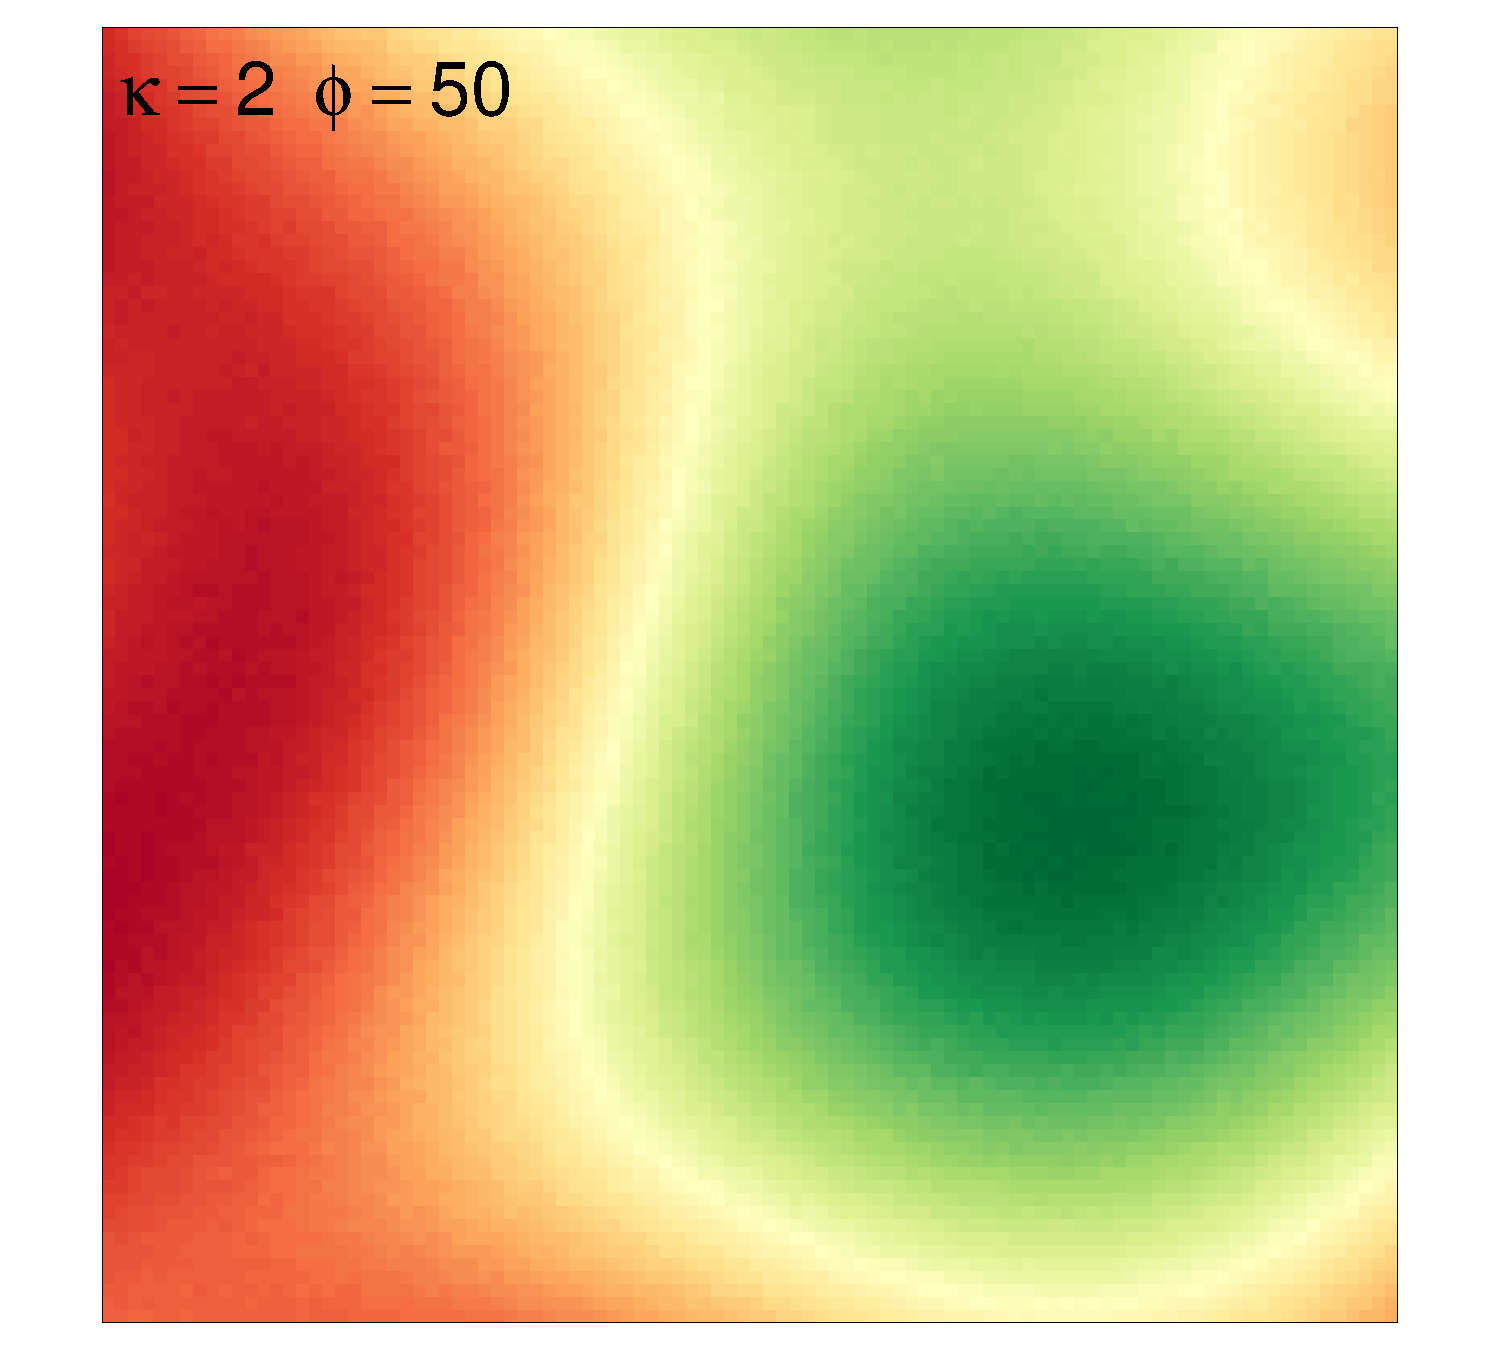
\includegraphics{Lecture_1_files/figure-beamer/unnamed-chunk-22-1.pdf}
\end{column}
\end{columns}
\end{frame}

\hypertarget{matuxe9rn-family}{%
\subsection{Matérn family}\label{matuxe9rn-family}}

\begin{frame}{Matérn family}
\large

\[\rho(u)=\{2^{\kappa-1}\Gamma(\kappa)\}^{-1}\left(\frac{u}{\phi}\right)^\kappa K_\kappa\left(\tfrac{u}{\phi}\right)\]

\small

\(\phi\) \ldots{} scale, \(\phi>0\)

\(\kappa\) \ldots{} order, \(\kappa>0\)

\(K_\kappa\) \ldots{} modifikovaná Besselova funkce druhého typu řádu
\(\kappa\)

\begin{columns}[T]
\begin{column}{0.5\textwidth}
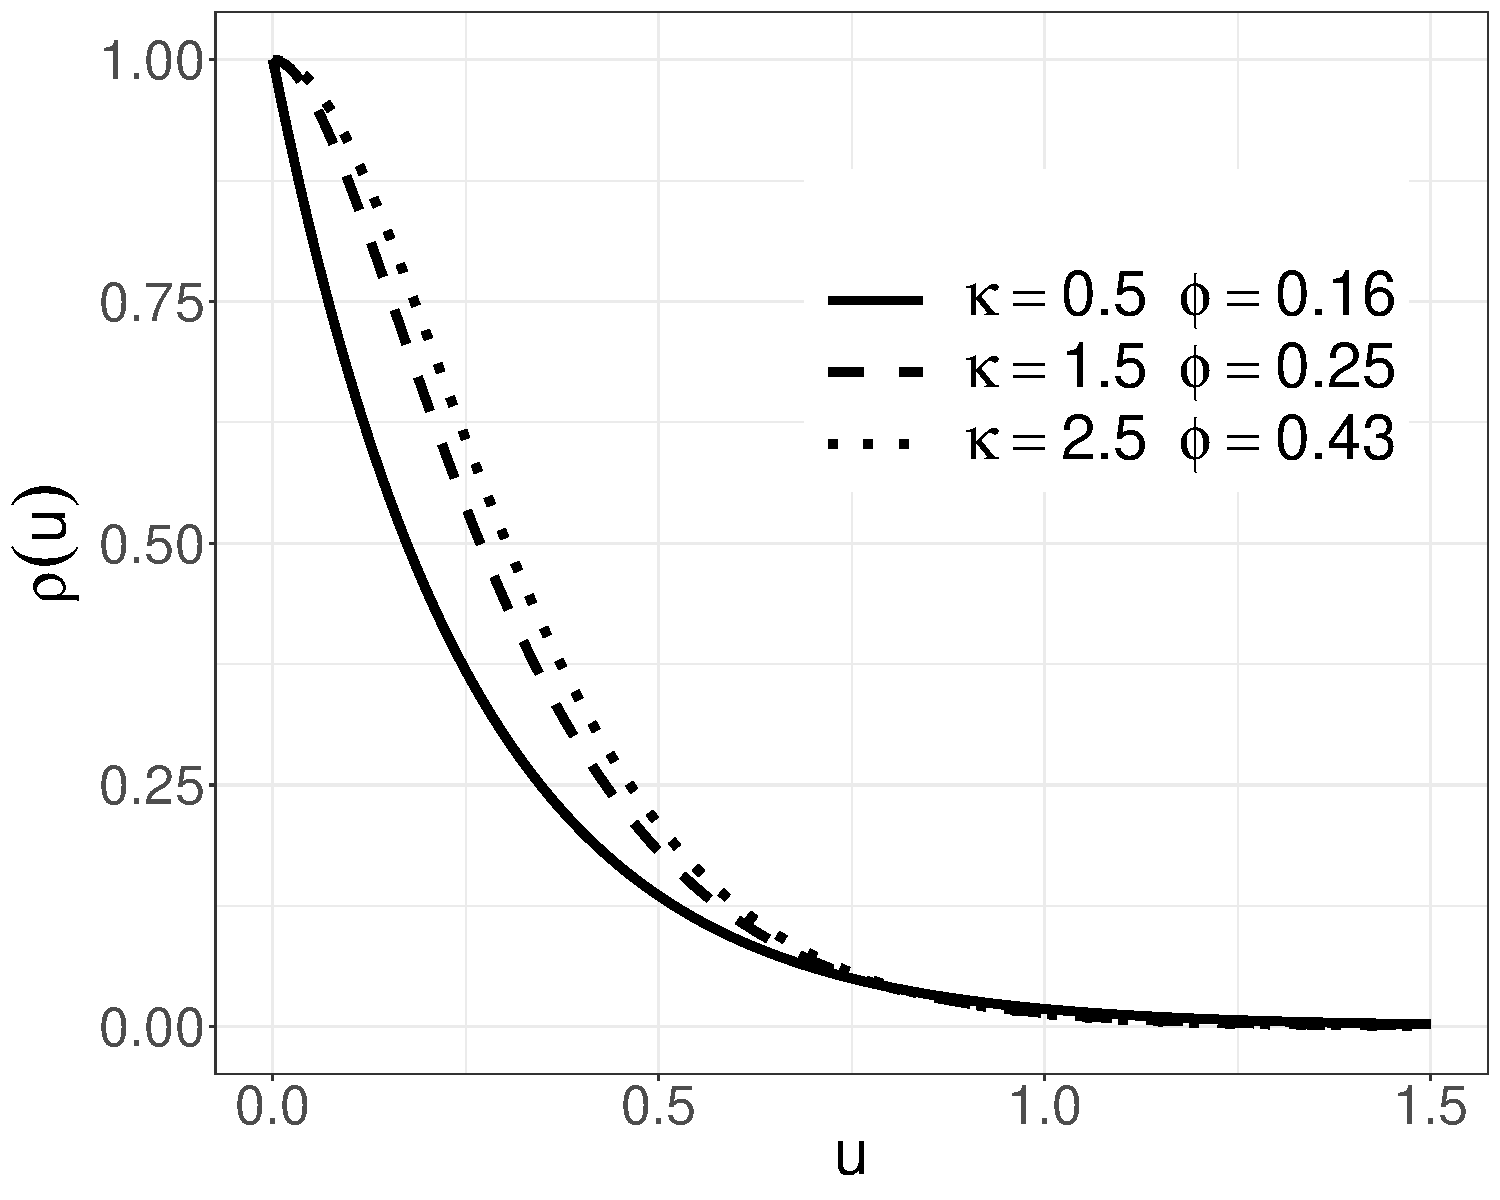
\includegraphics{Lecture_1_files/figure-beamer/unnamed-chunk-23-1.pdf}
\end{column}

\begin{column}{0.5\textwidth}
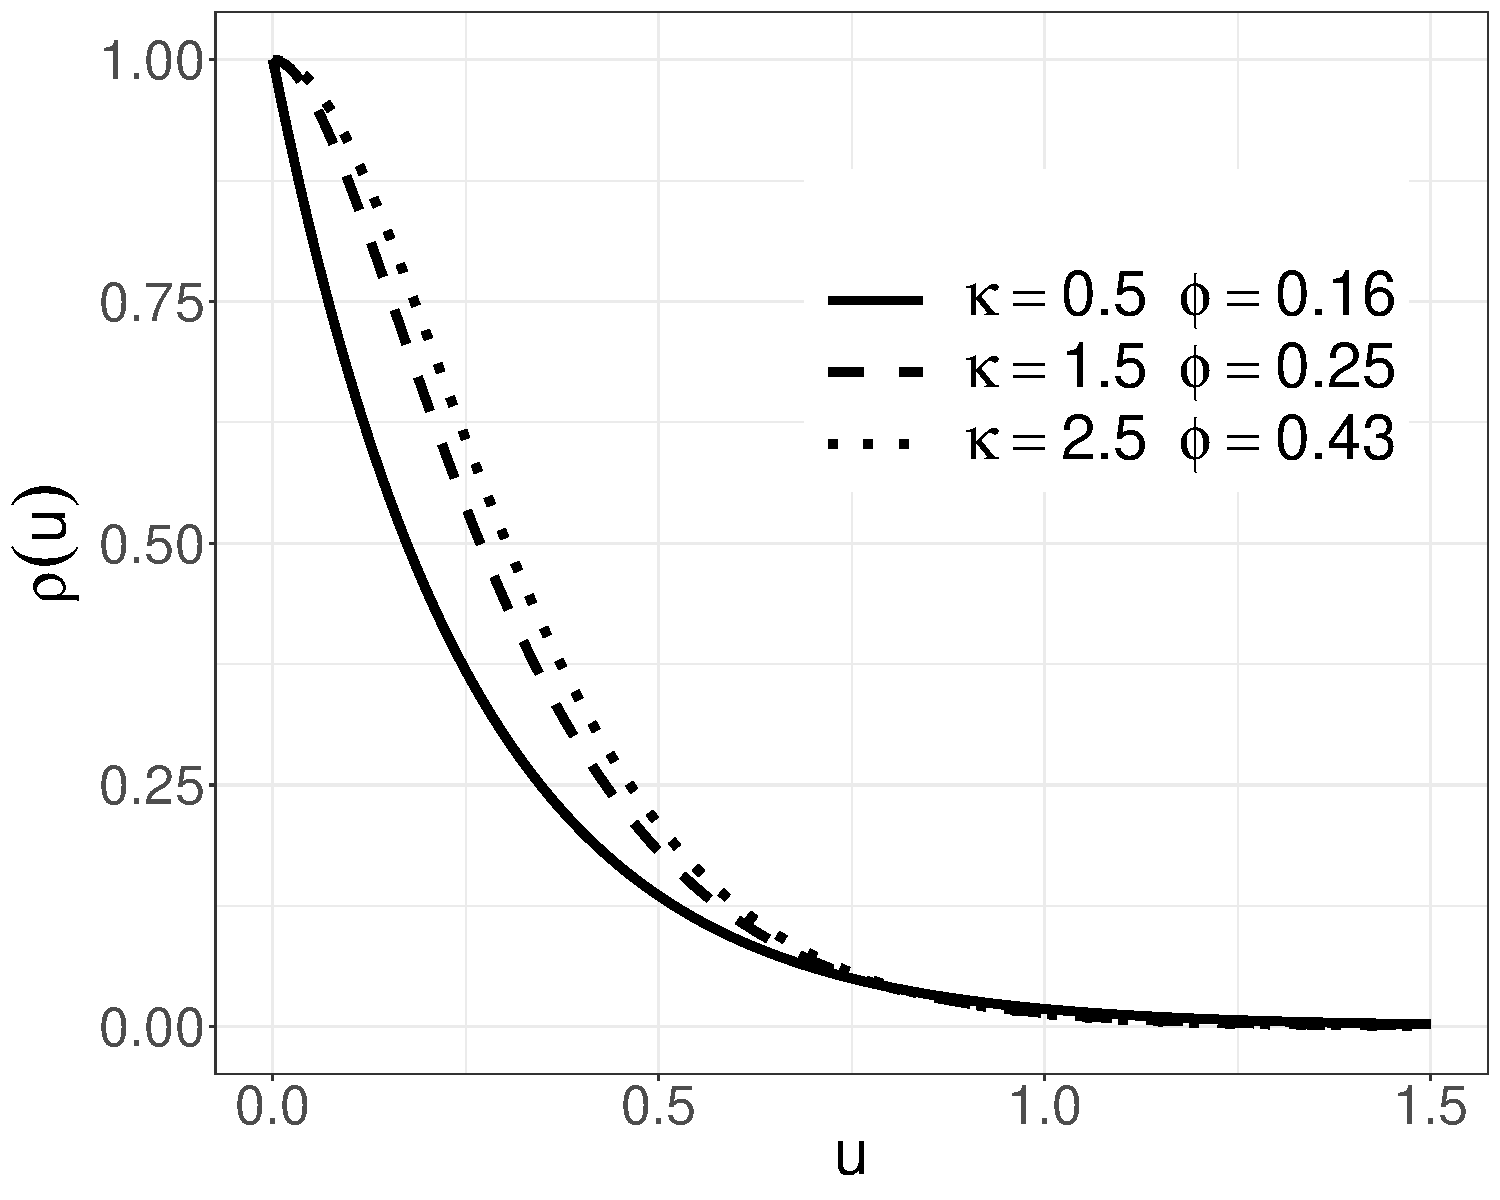
\includegraphics{Lecture_1_files/figure-beamer/unnamed-chunk-24-1.pdf}
\end{column}
\end{columns}
\end{frame}

\hypertarget{matuxe9rn-family-1}{%
\subsection{Matérn family}\label{matuxe9rn-family-1}}

\begin{frame}{Matérn family}
\large

\[\rho(u)=\{2^{\kappa-1}\Gamma(\kappa)\}^{-1}\left(\frac{u}{\phi}\right)^\kappa K_\kappa\left(\tfrac{u}{\phi}\right)\]

\small

\(\phi\) \ldots{} scale, \(\phi>0\)

\(\kappa\) \ldots{} order, \(\kappa>0\)

\(K_\kappa\) \ldots{} modifikovaná Besselova funkce druhého typu řádu
\(\kappa\)

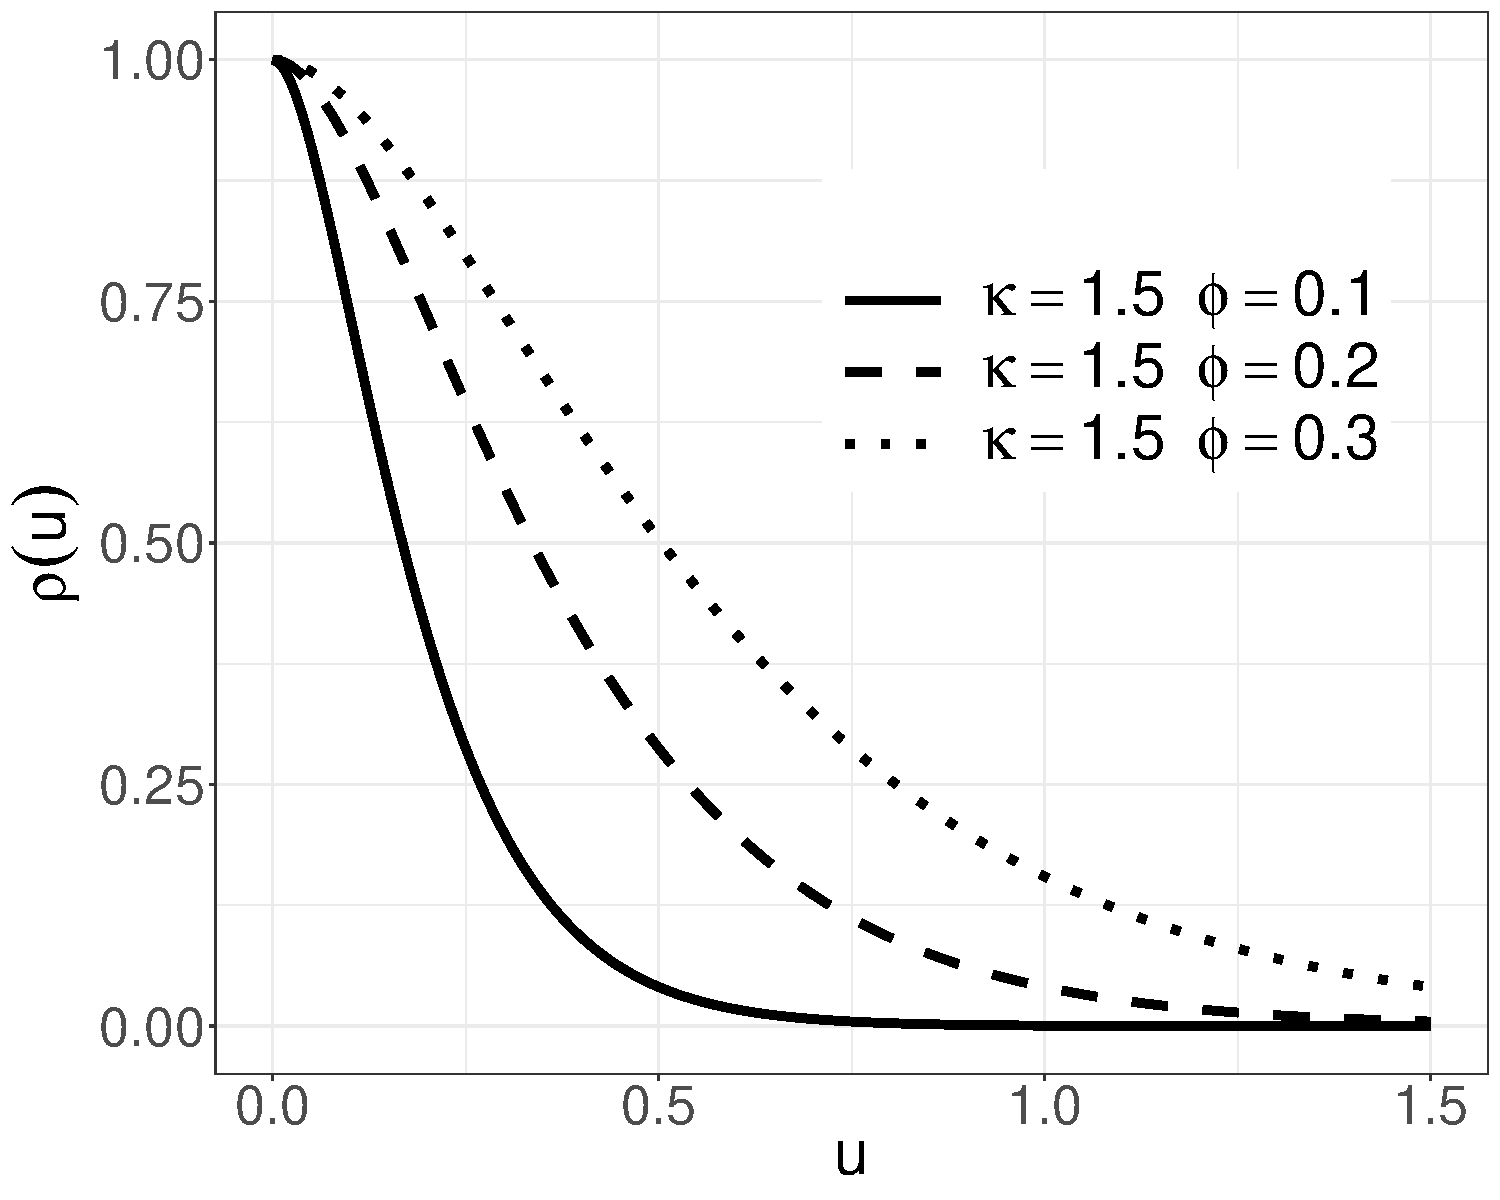
\includegraphics{Lecture_1_files/figure-beamer/unnamed-chunk-25-1.pdf}
\end{frame}

\hypertarget{matuxe9rn-family-2}{%
\subsection{Matérn family}\label{matuxe9rn-family-2}}

\begin{frame}{Matérn family}
\small

\begin{columns}[T]
\begin{column}{0.33\textwidth}
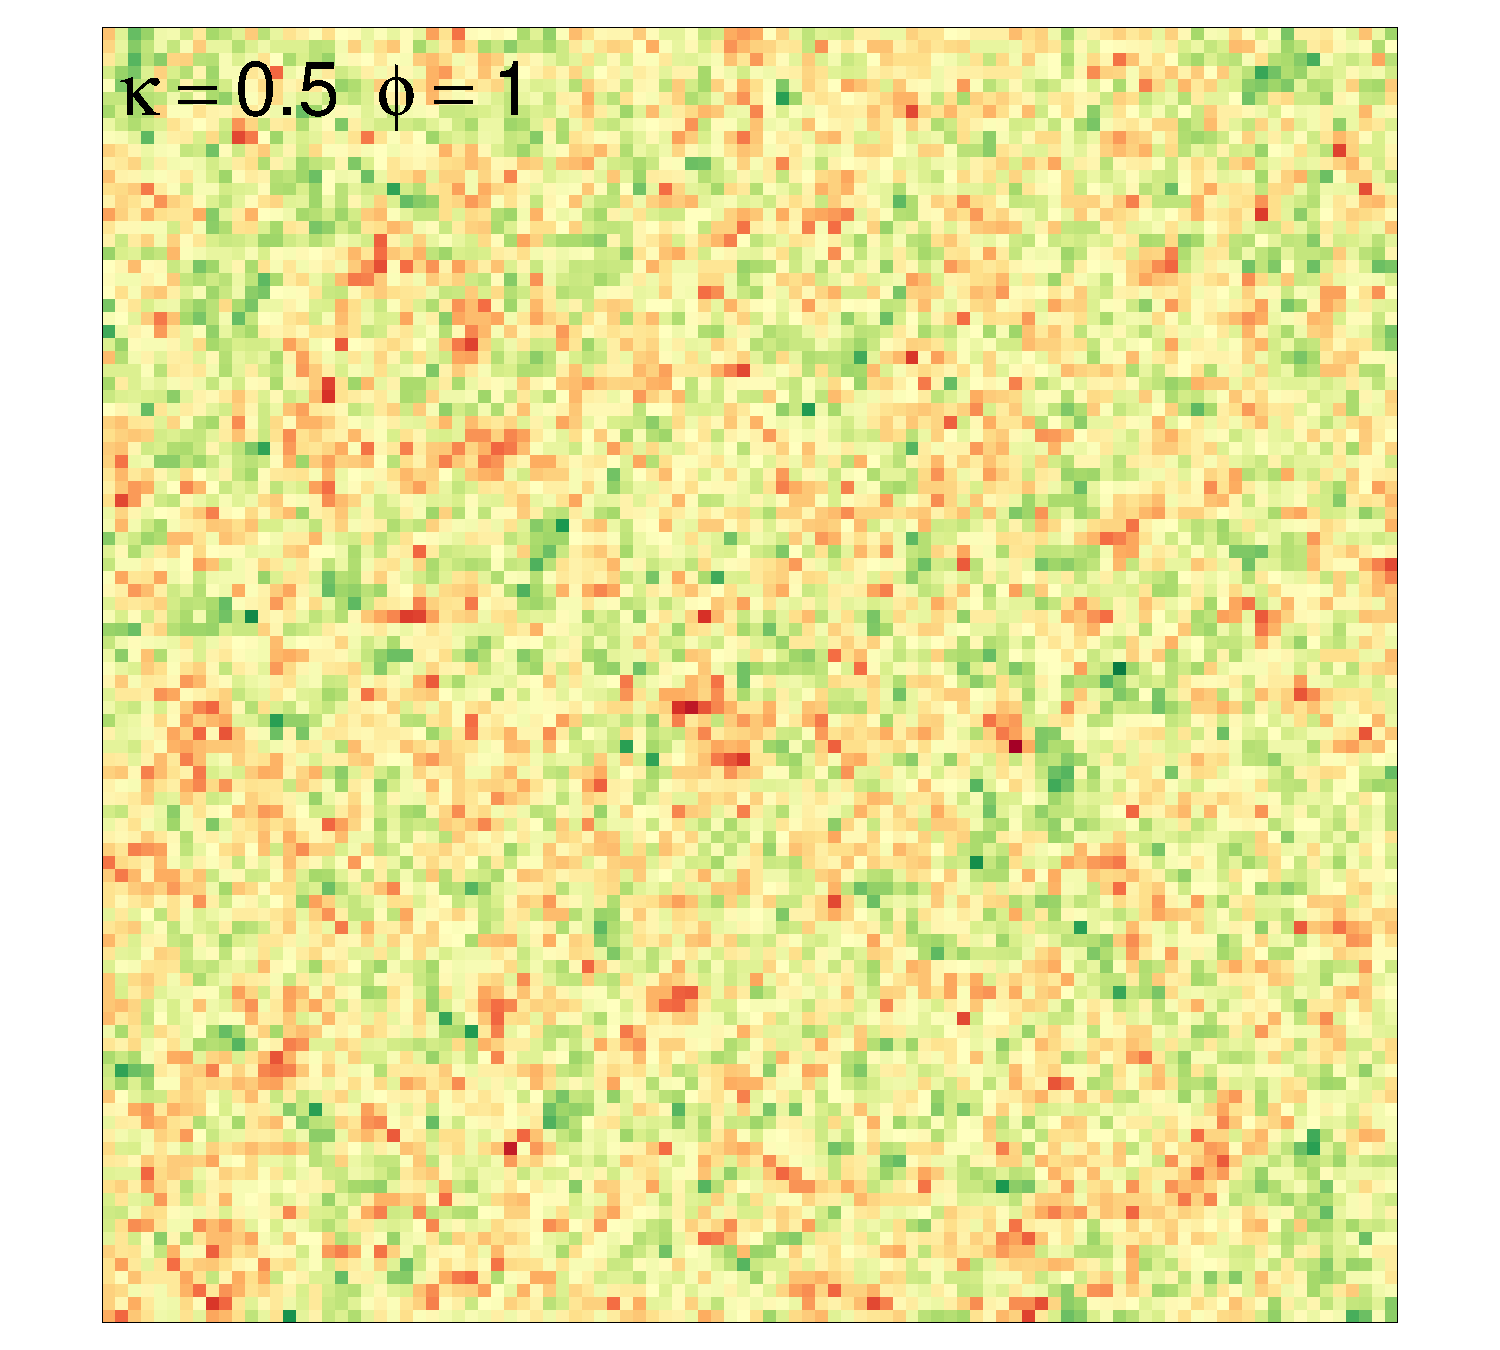
\includegraphics{Lecture_1_files/figure-beamer/unnamed-chunk-26-1.pdf}
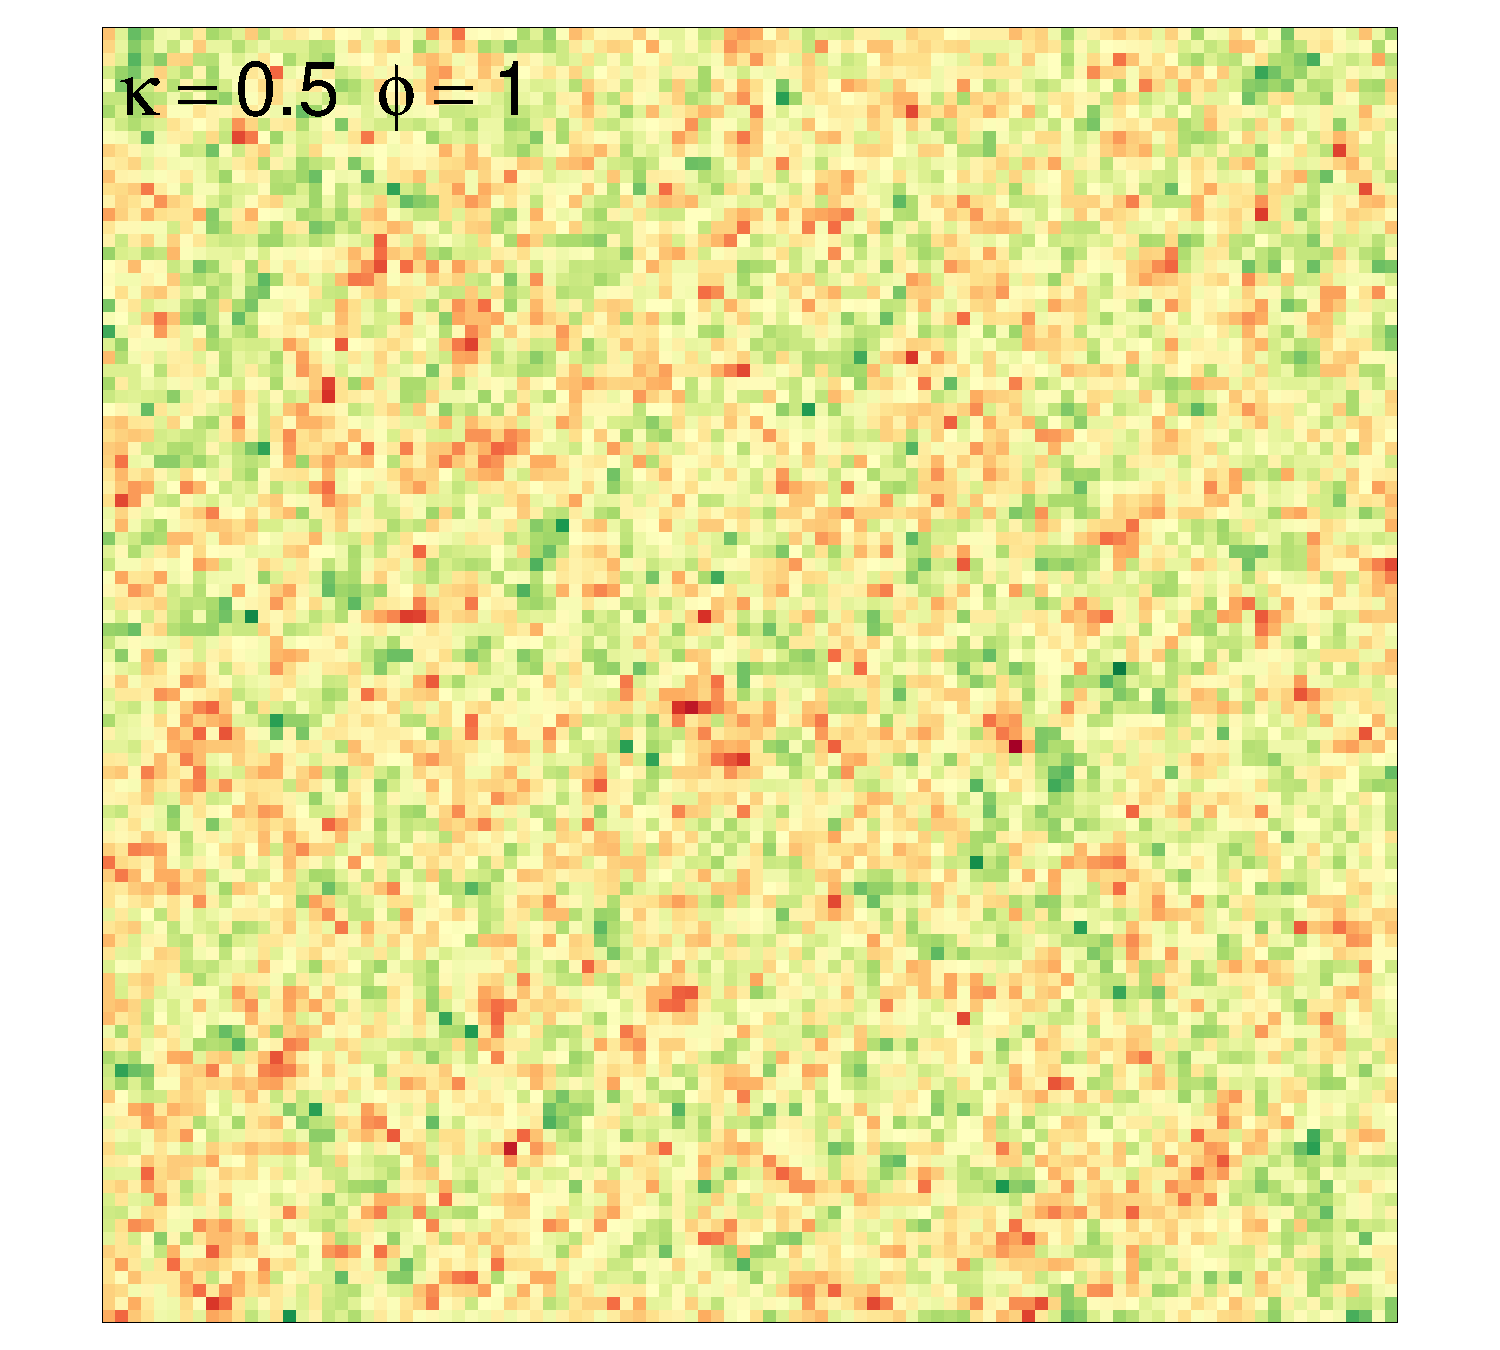
\includegraphics{Lecture_1_files/figure-beamer/unnamed-chunk-27-1.pdf}
\end{column}

\begin{column}{0.33\textwidth}
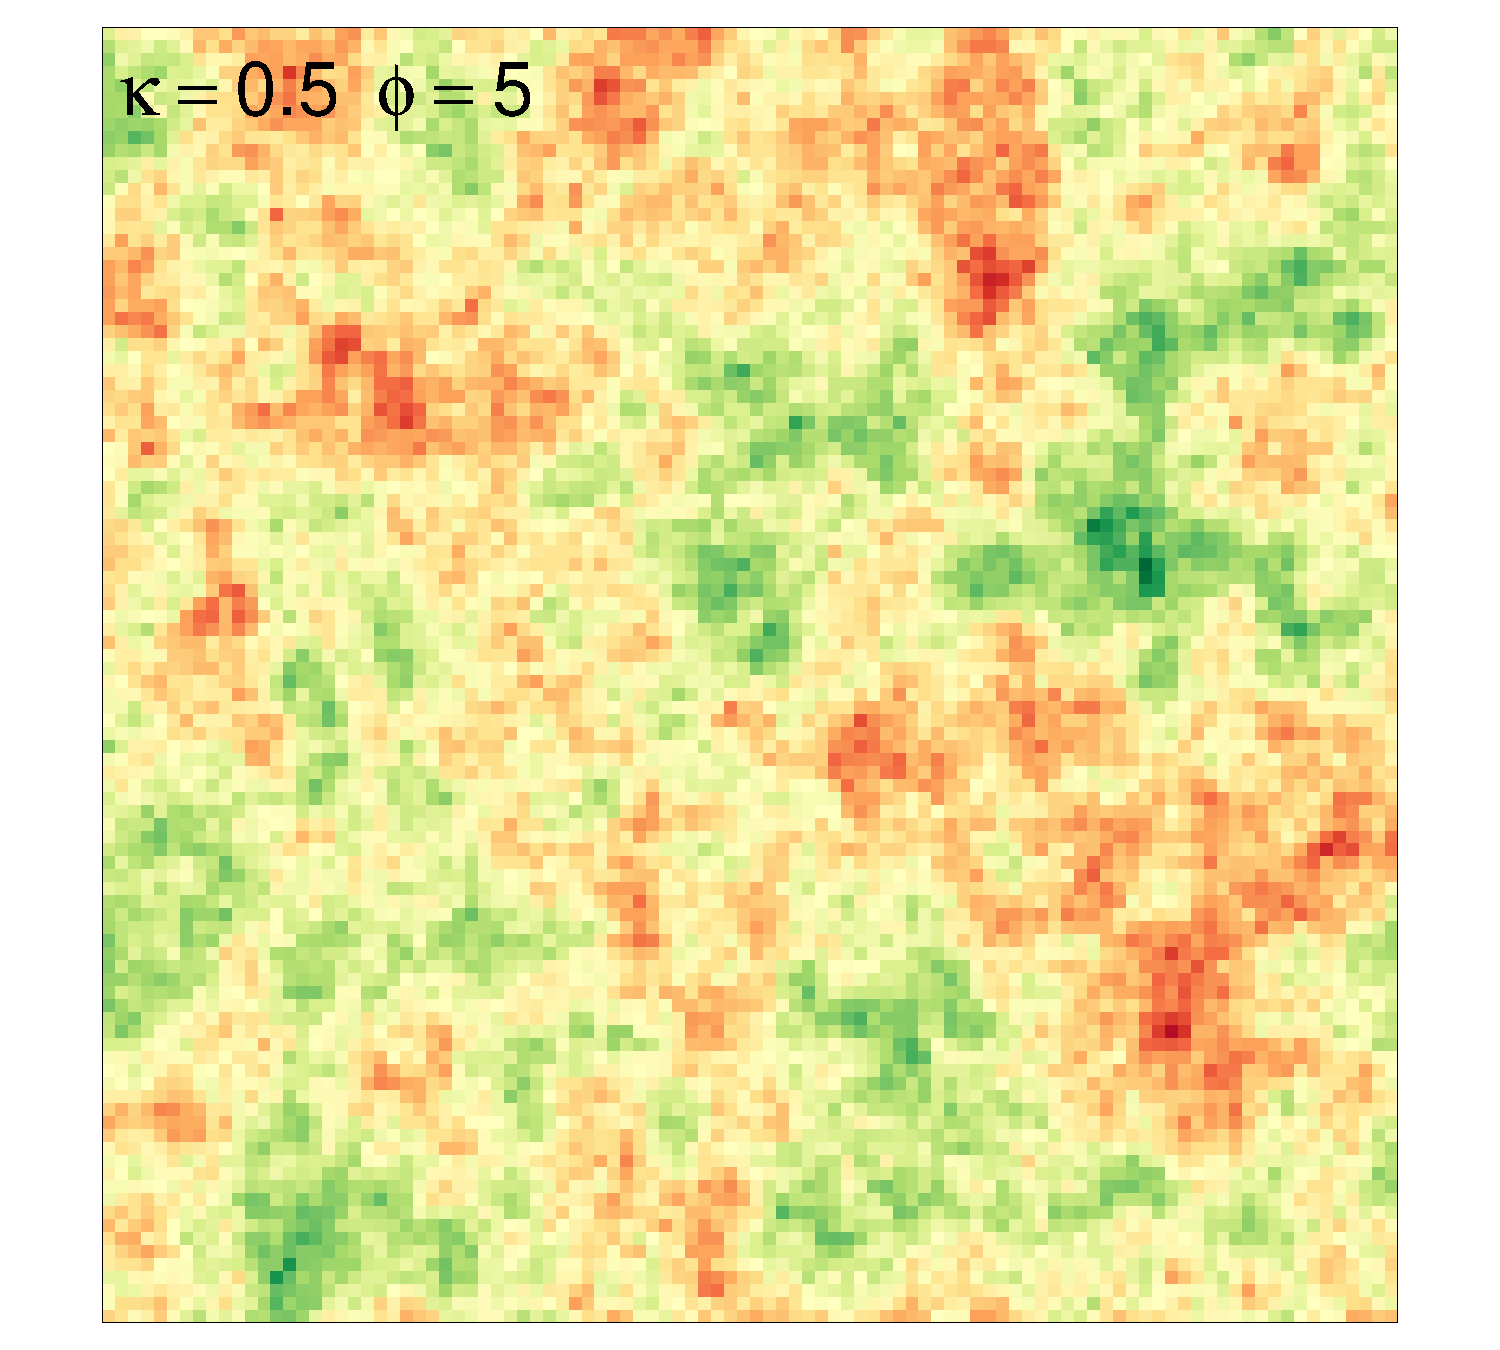
\includegraphics{Lecture_1_files/figure-beamer/unnamed-chunk-28-1.pdf}

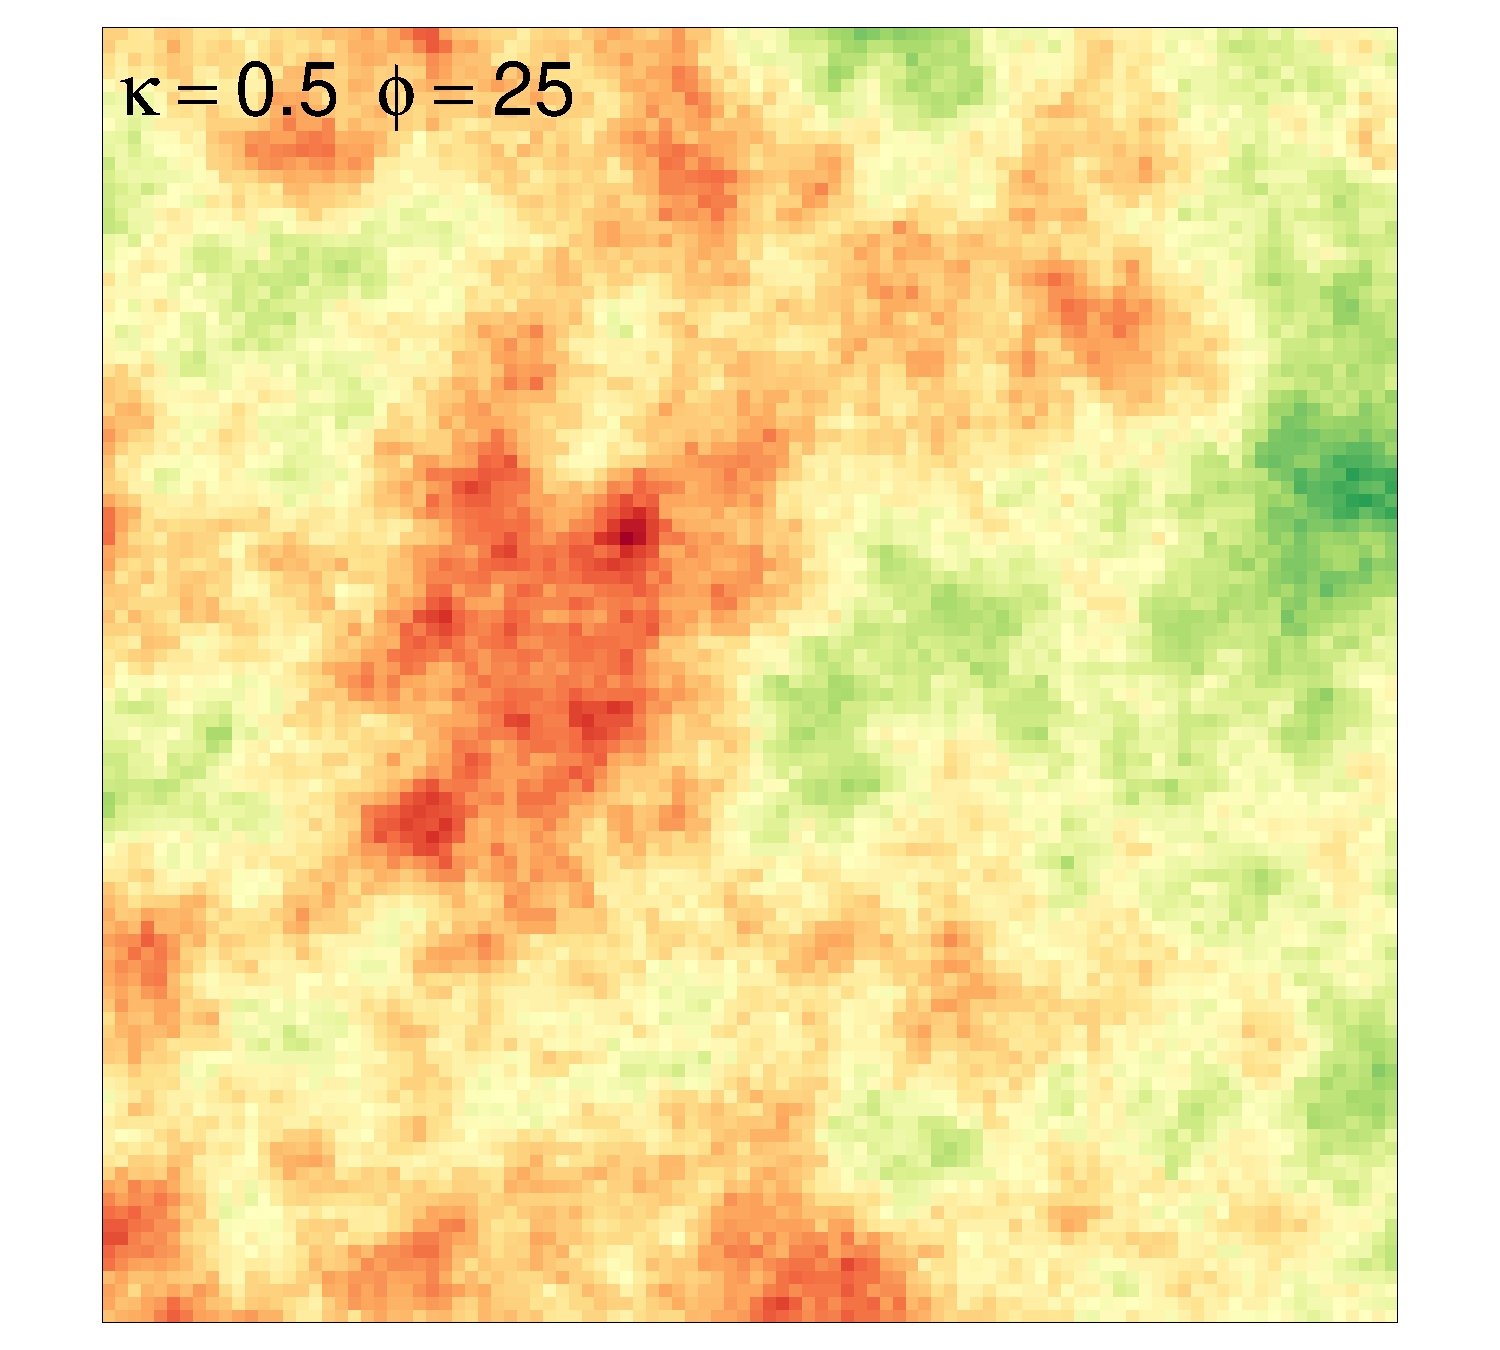
\includegraphics{Lecture_1_files/figure-beamer/unnamed-chunk-29-1.pdf}
\end{column}

\begin{column}{0.33\textwidth}
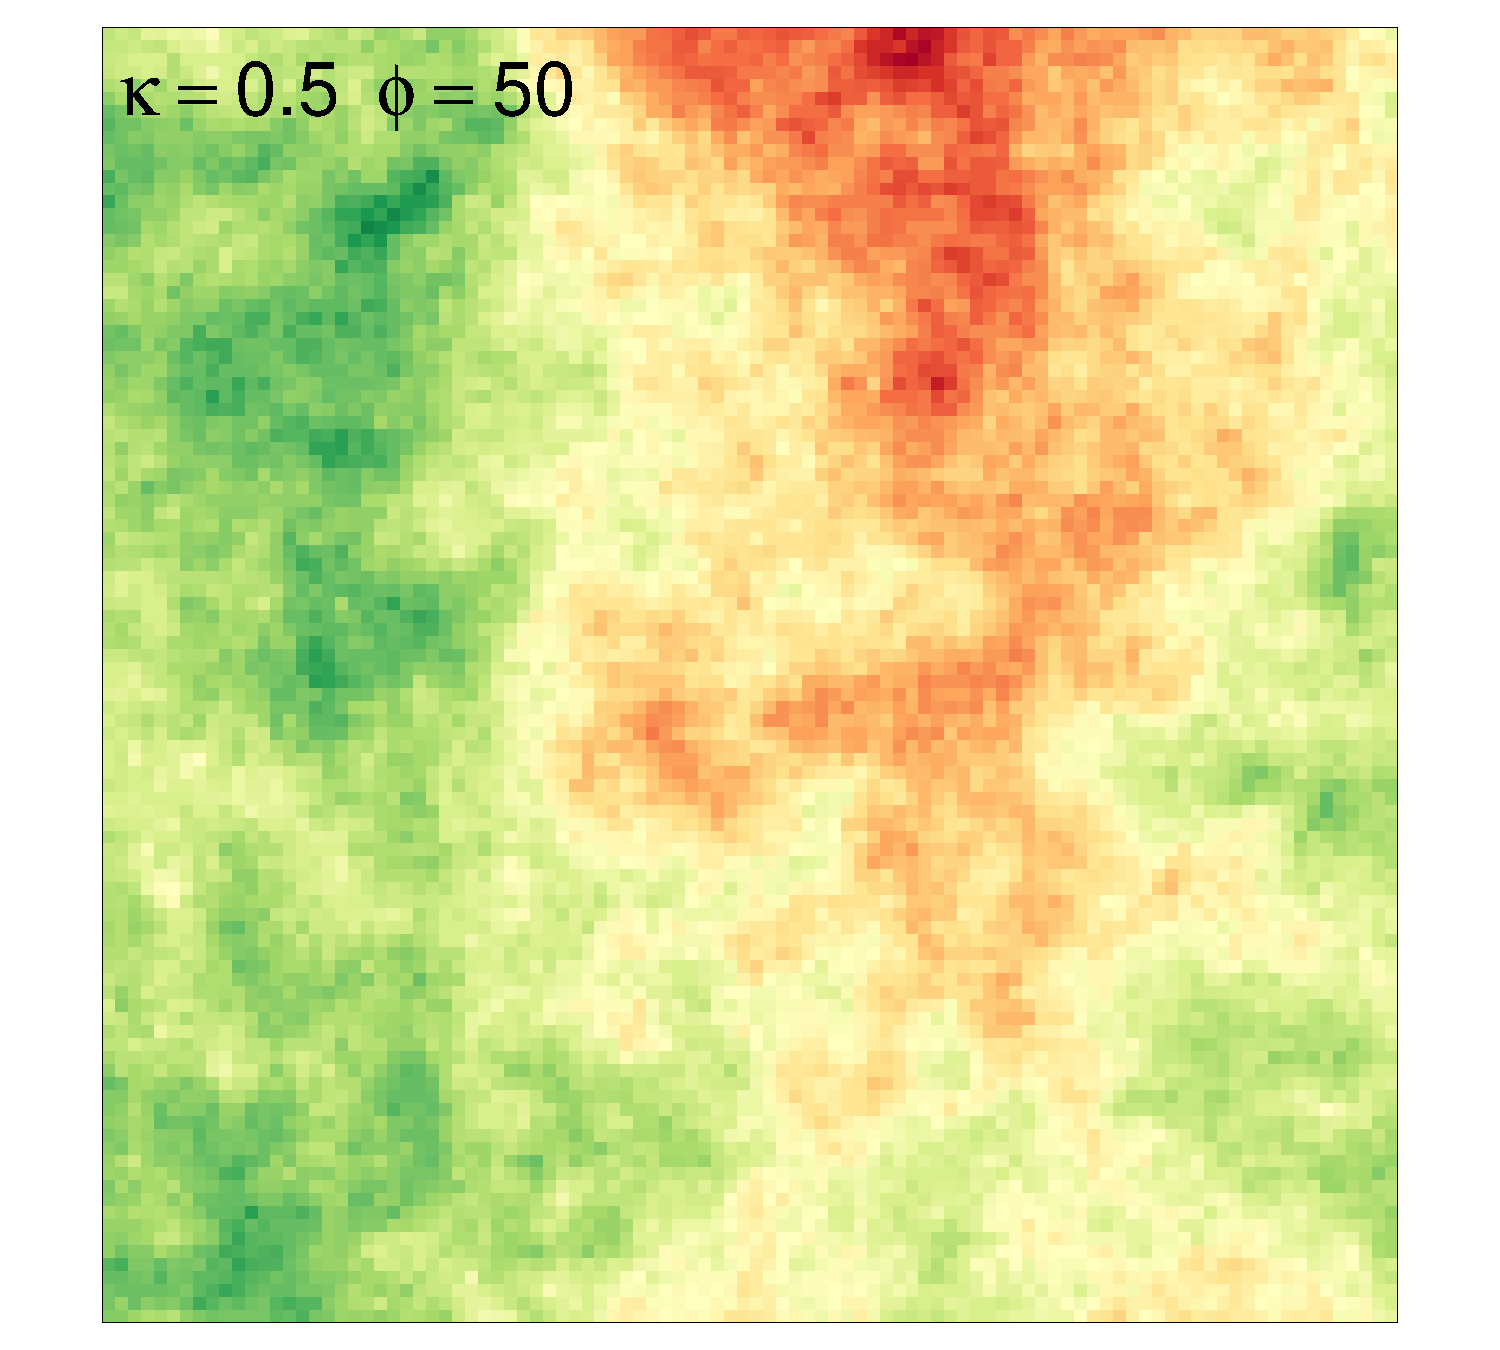
\includegraphics{Lecture_1_files/figure-beamer/unnamed-chunk-30-1.pdf}

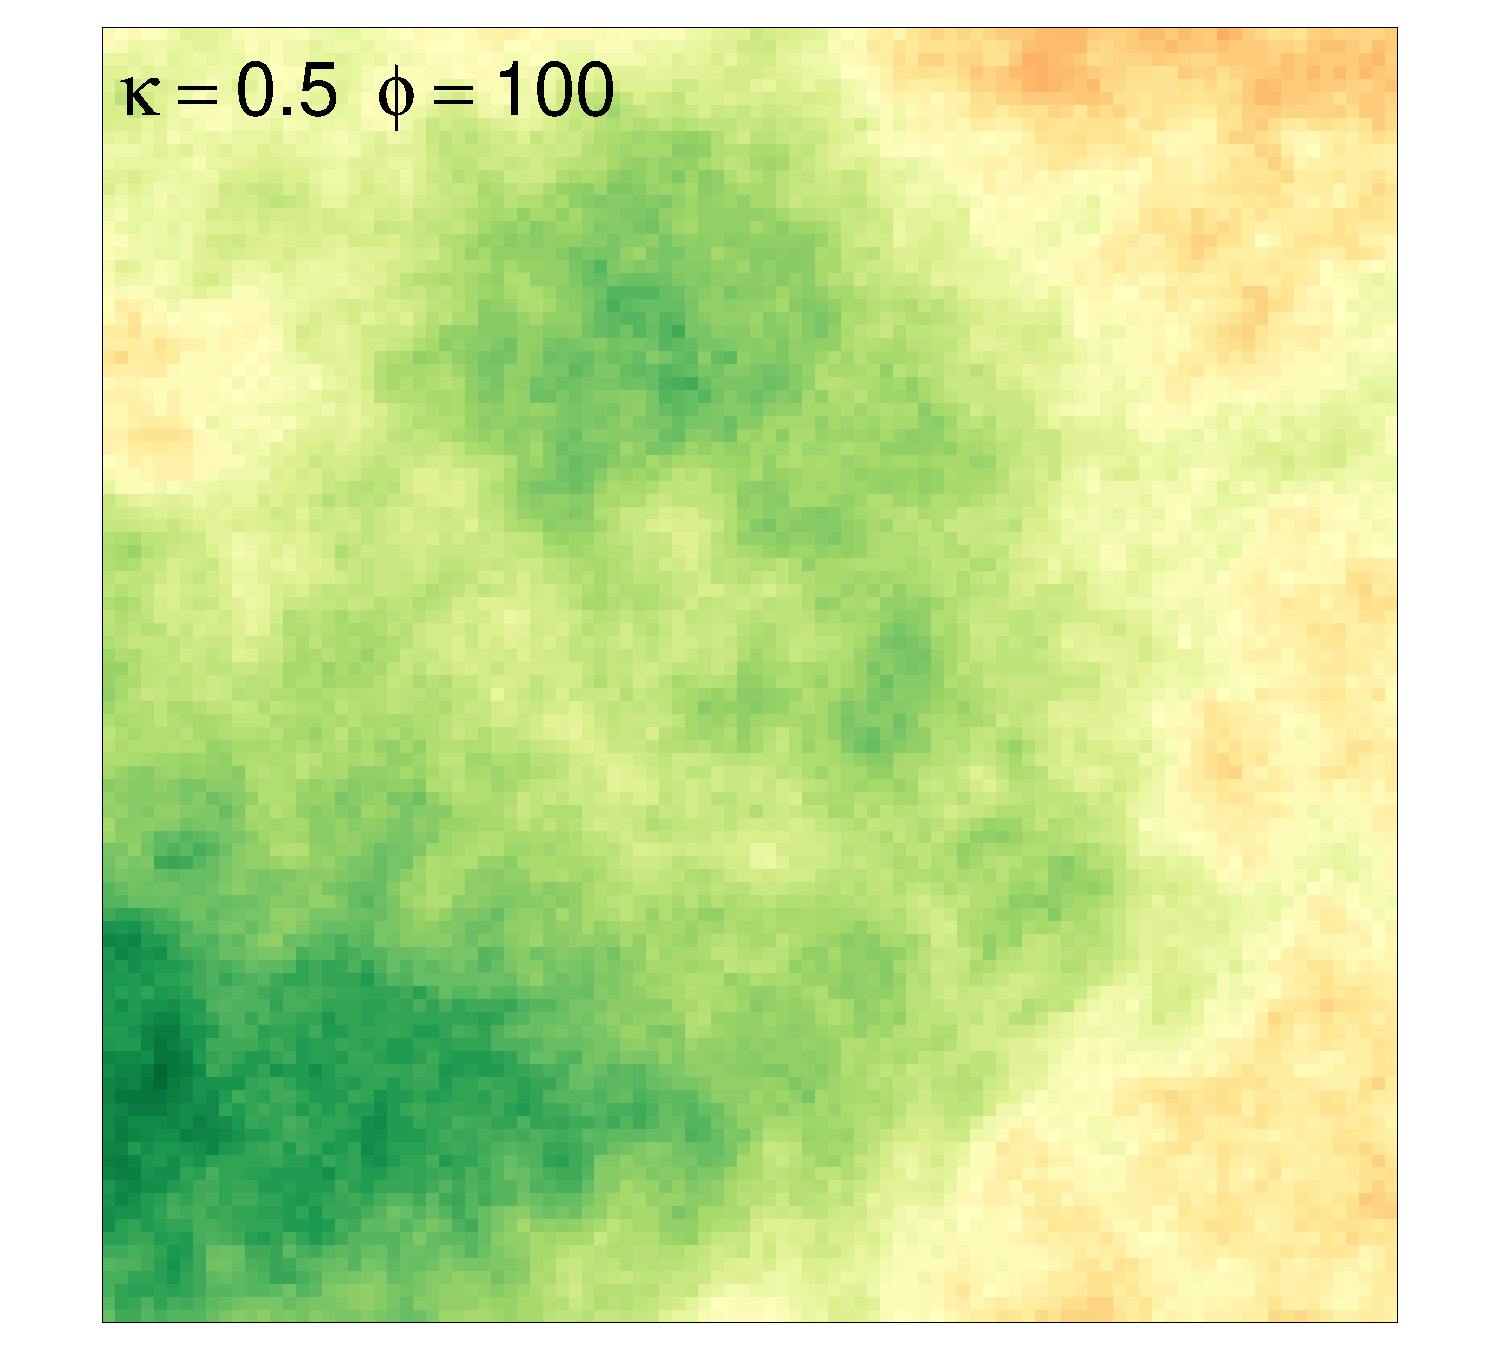
\includegraphics{Lecture_1_files/figure-beamer/unnamed-chunk-31-1.pdf}
\end{column}
\end{columns}
\end{frame}

\hypertarget{matuxe9rn-family-3}{%
\subsection{Matérn family}\label{matuxe9rn-family-3}}

\begin{frame}{Matérn family}
\small

\begin{columns}[T]
\begin{column}{0.33\textwidth}
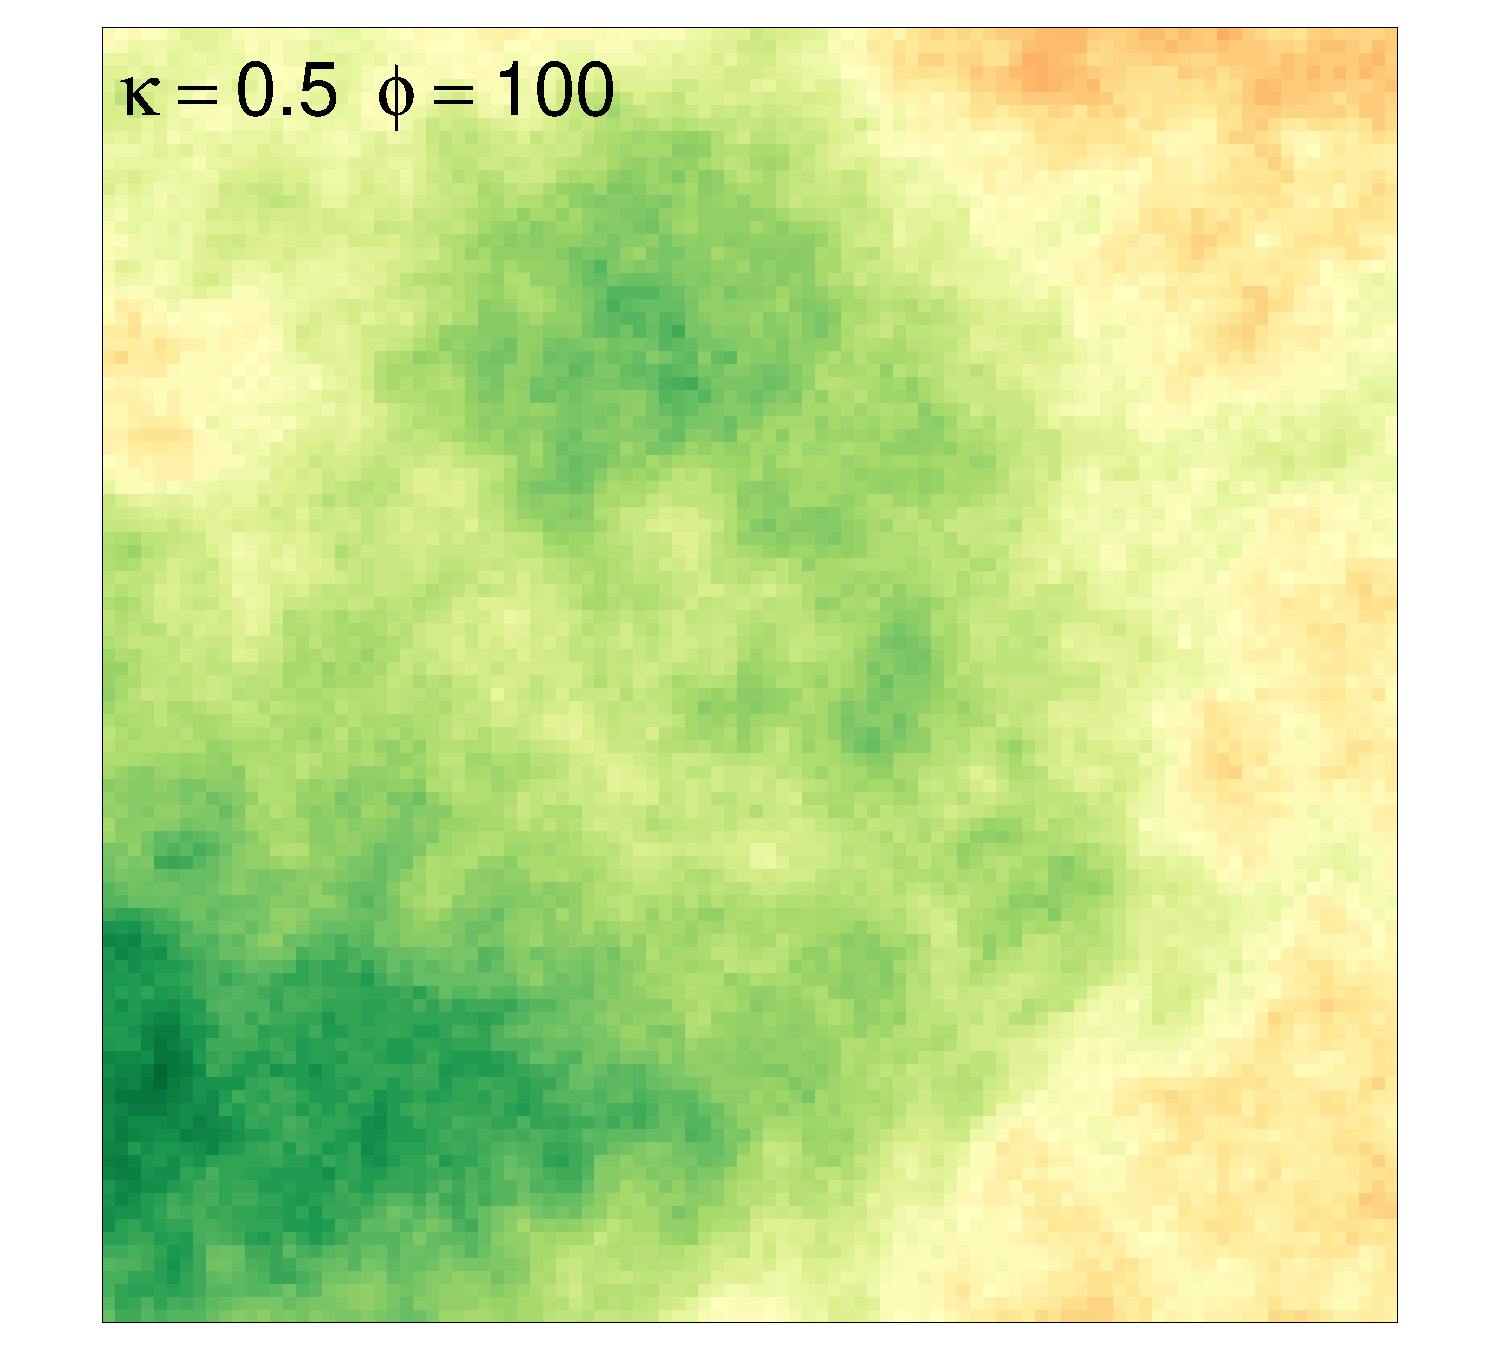
\includegraphics{Lecture_1_files/figure-beamer/unnamed-chunk-32-1.pdf}
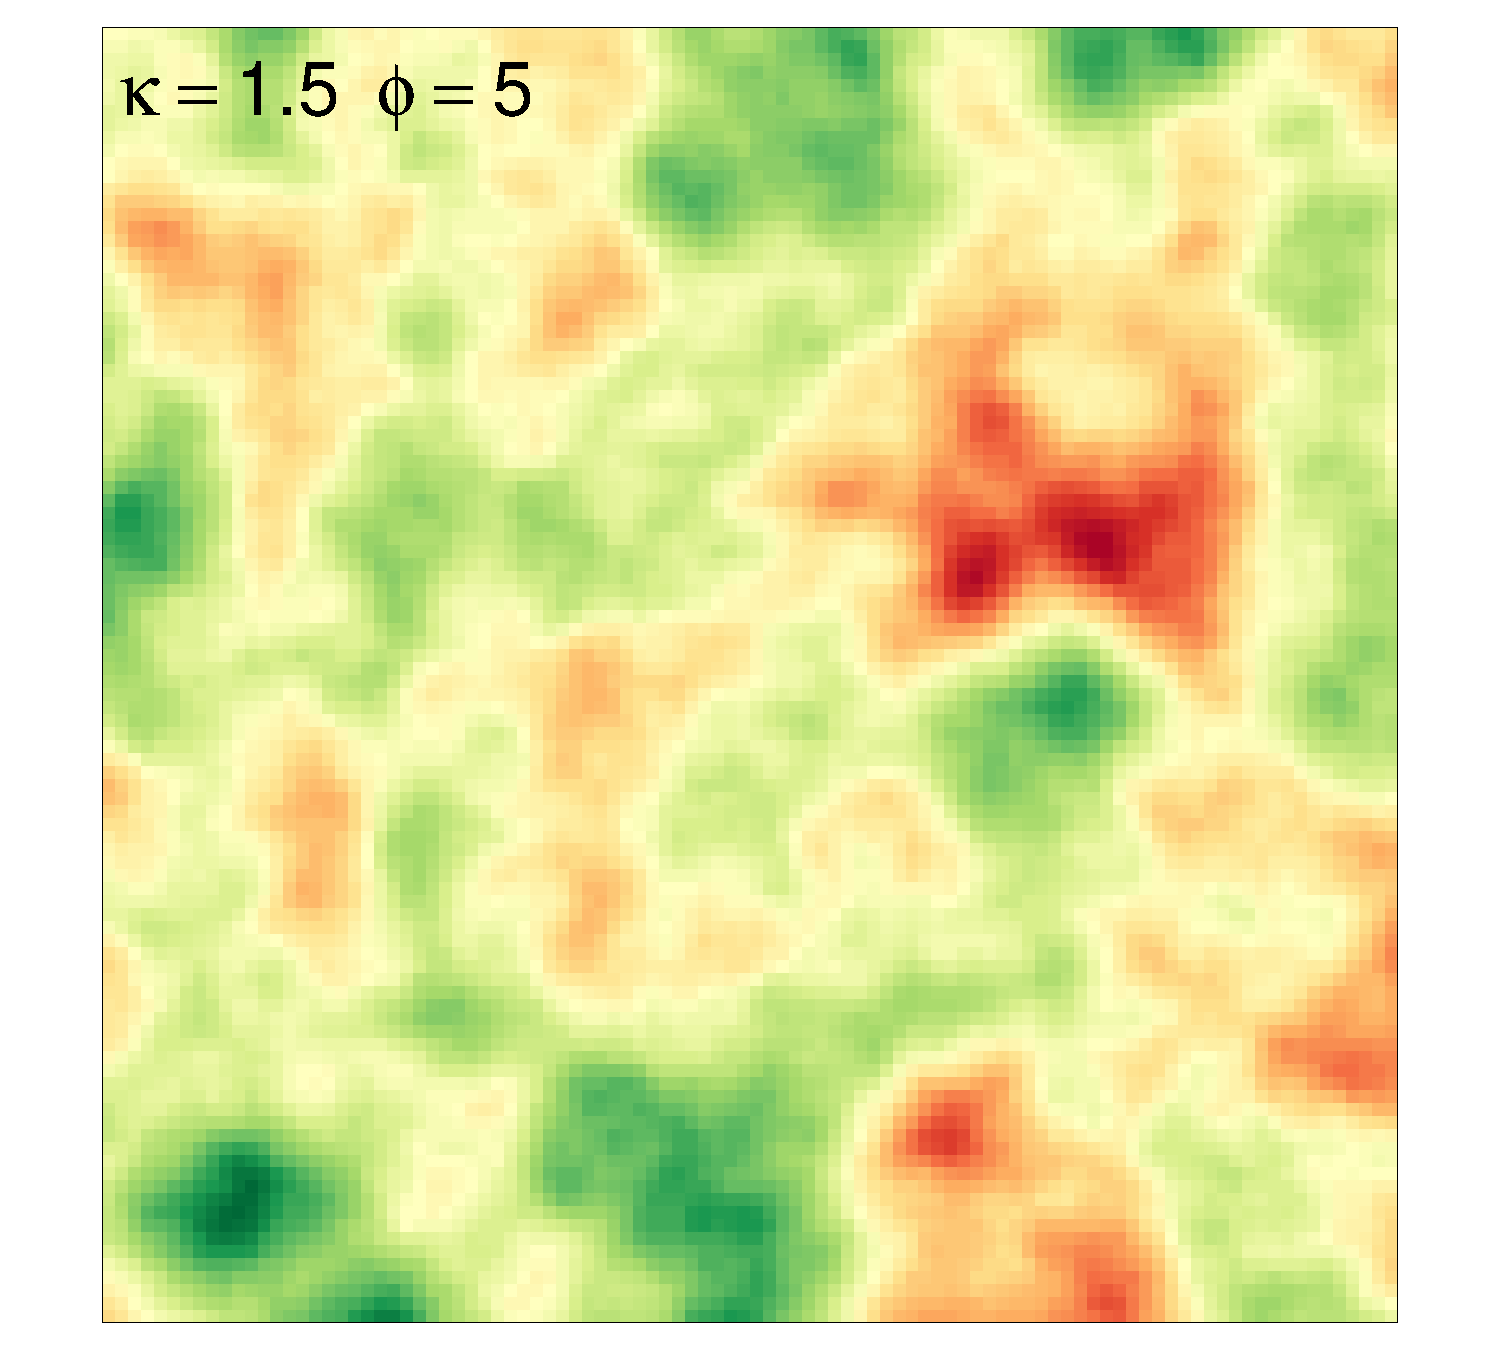
\includegraphics{Lecture_1_files/figure-beamer/unnamed-chunk-33-1.pdf}
\end{column}

\begin{column}{0.33\textwidth}
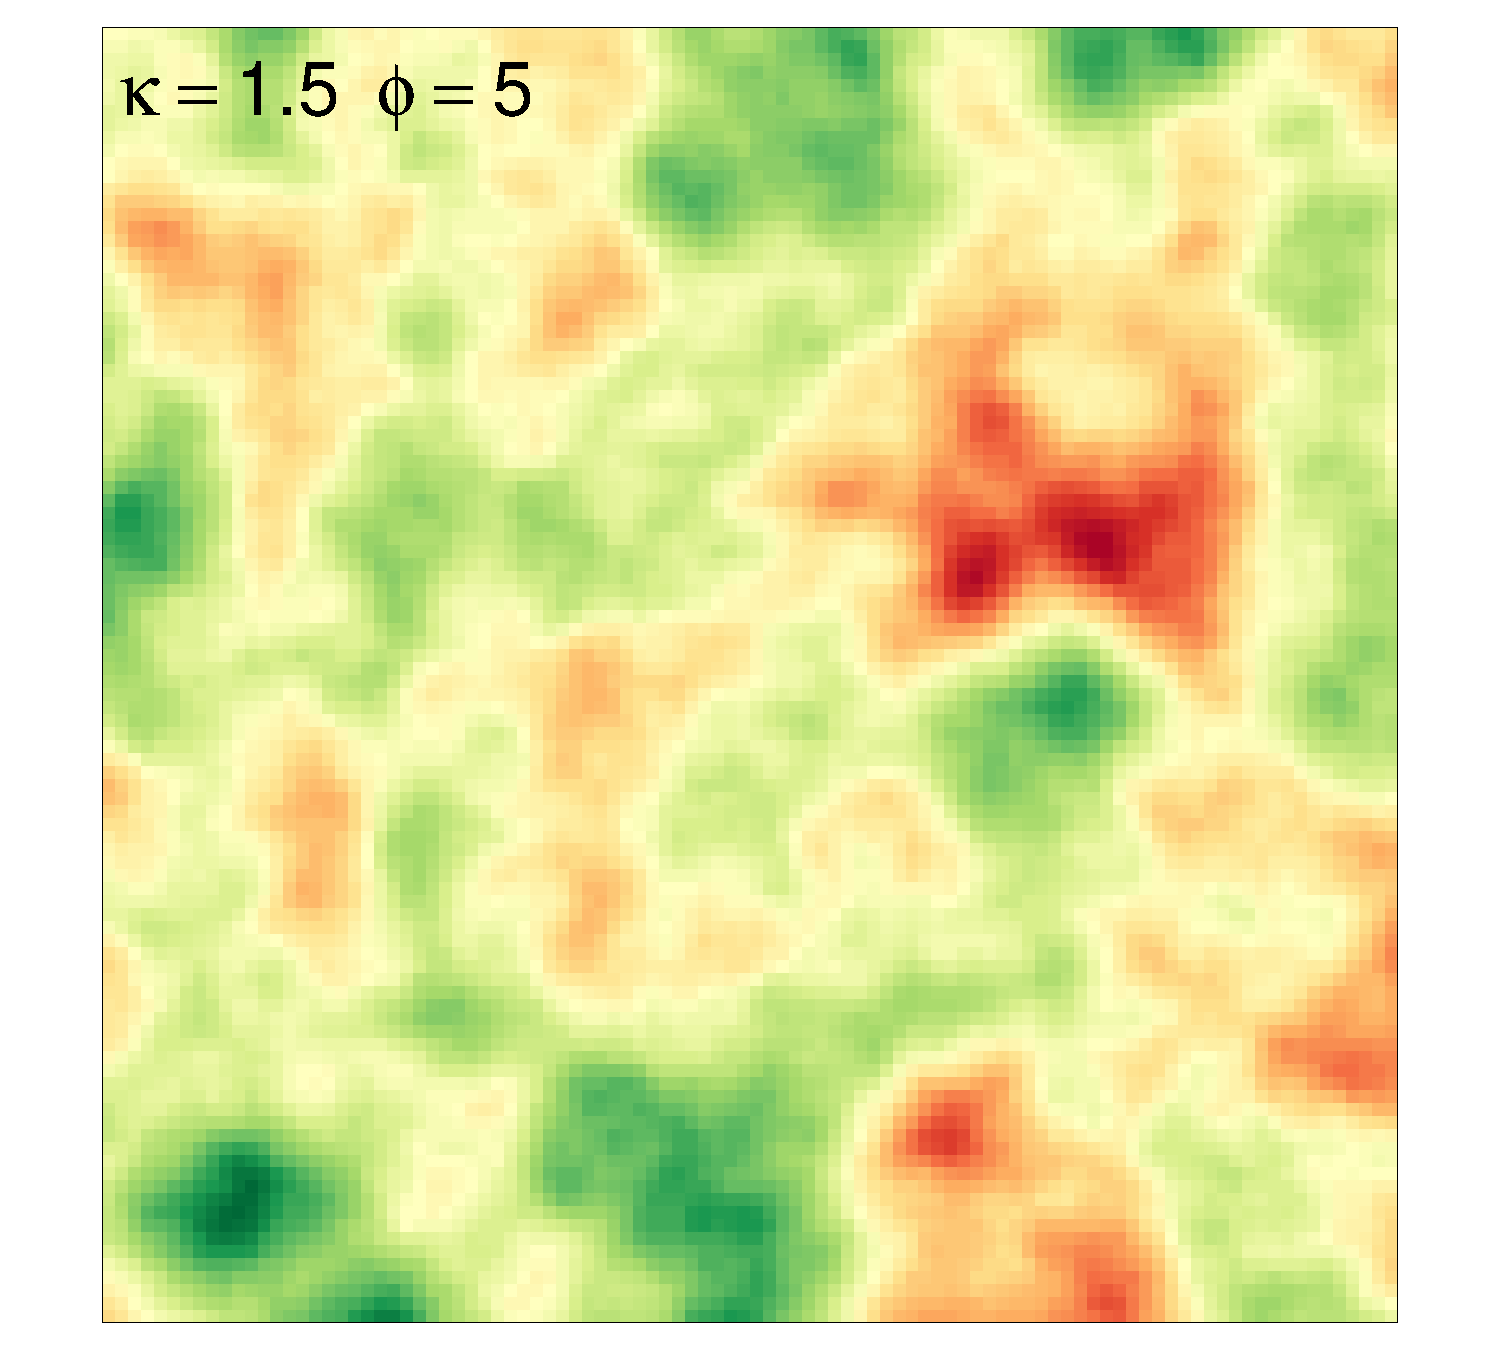
\includegraphics{Lecture_1_files/figure-beamer/unnamed-chunk-34-1.pdf}

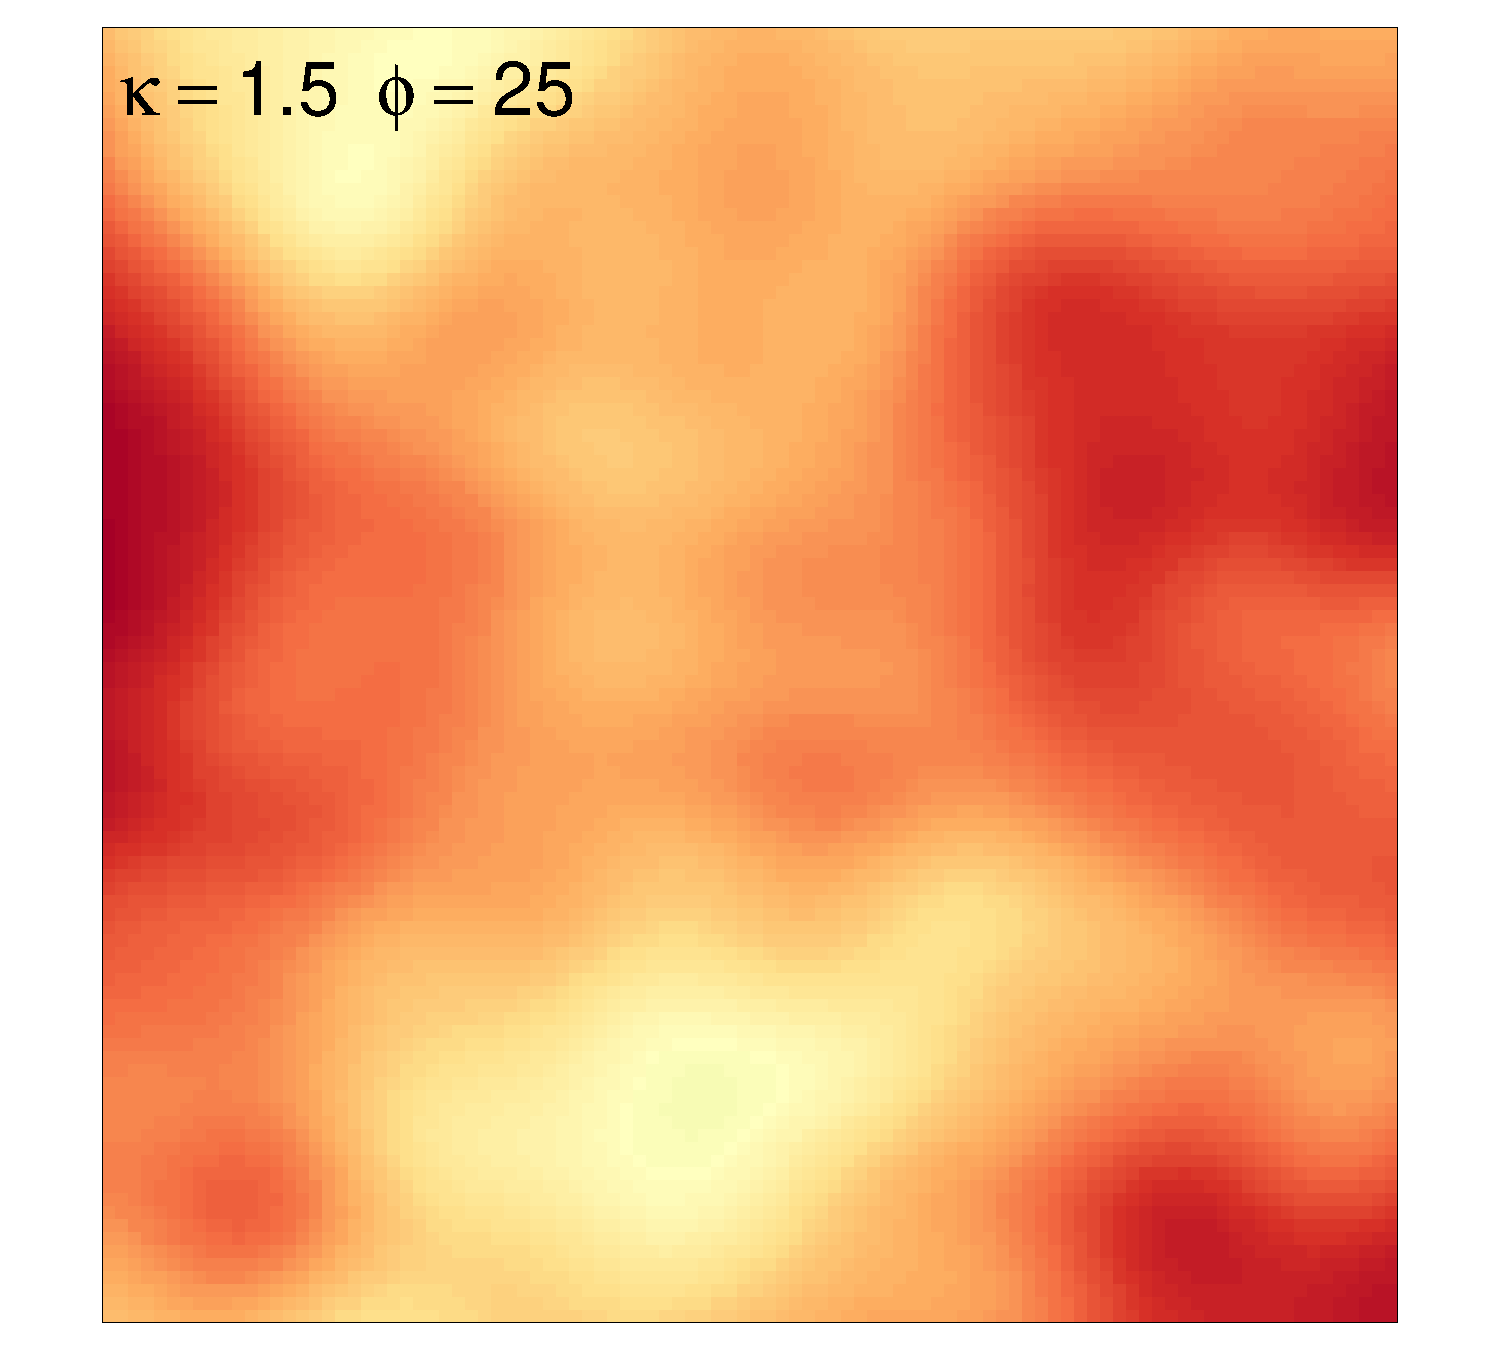
\includegraphics{Lecture_1_files/figure-beamer/unnamed-chunk-35-1.pdf}
\end{column}

\begin{column}{0.33\textwidth}
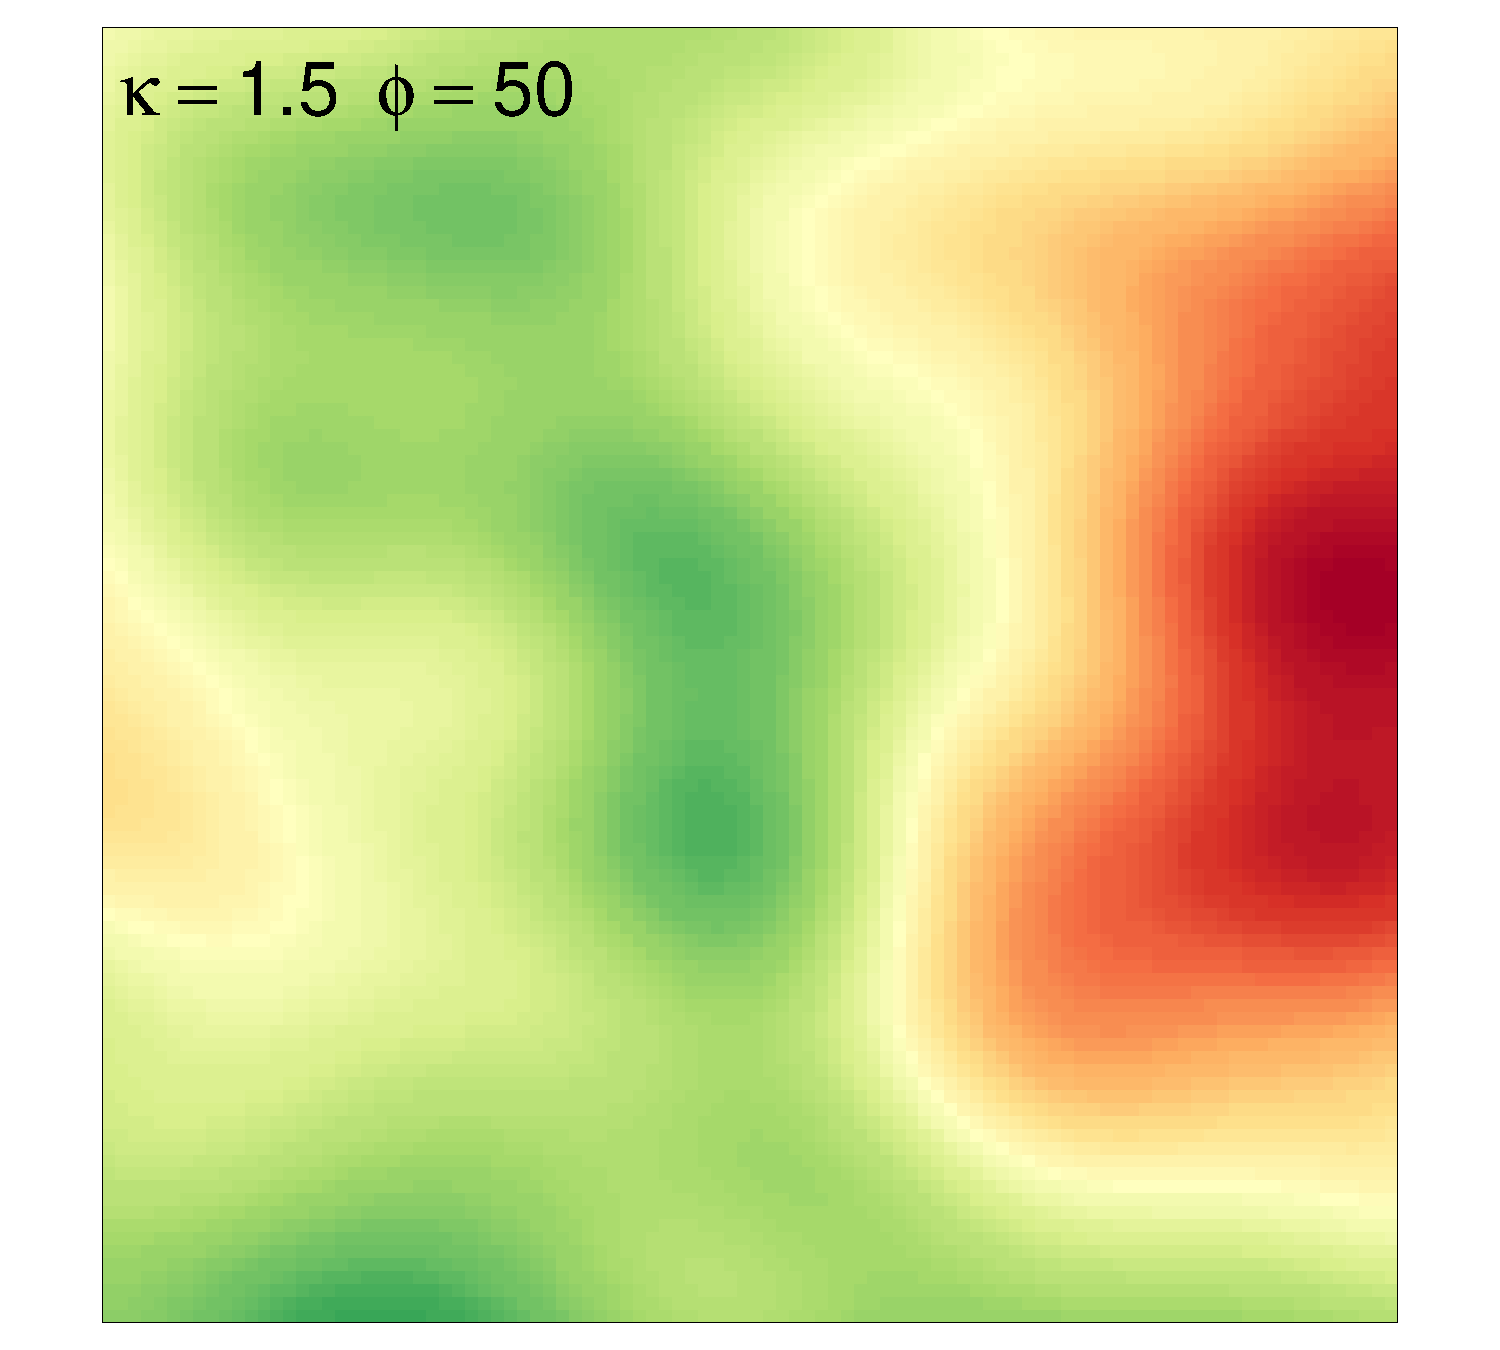
\includegraphics{Lecture_1_files/figure-beamer/unnamed-chunk-36-1.pdf}

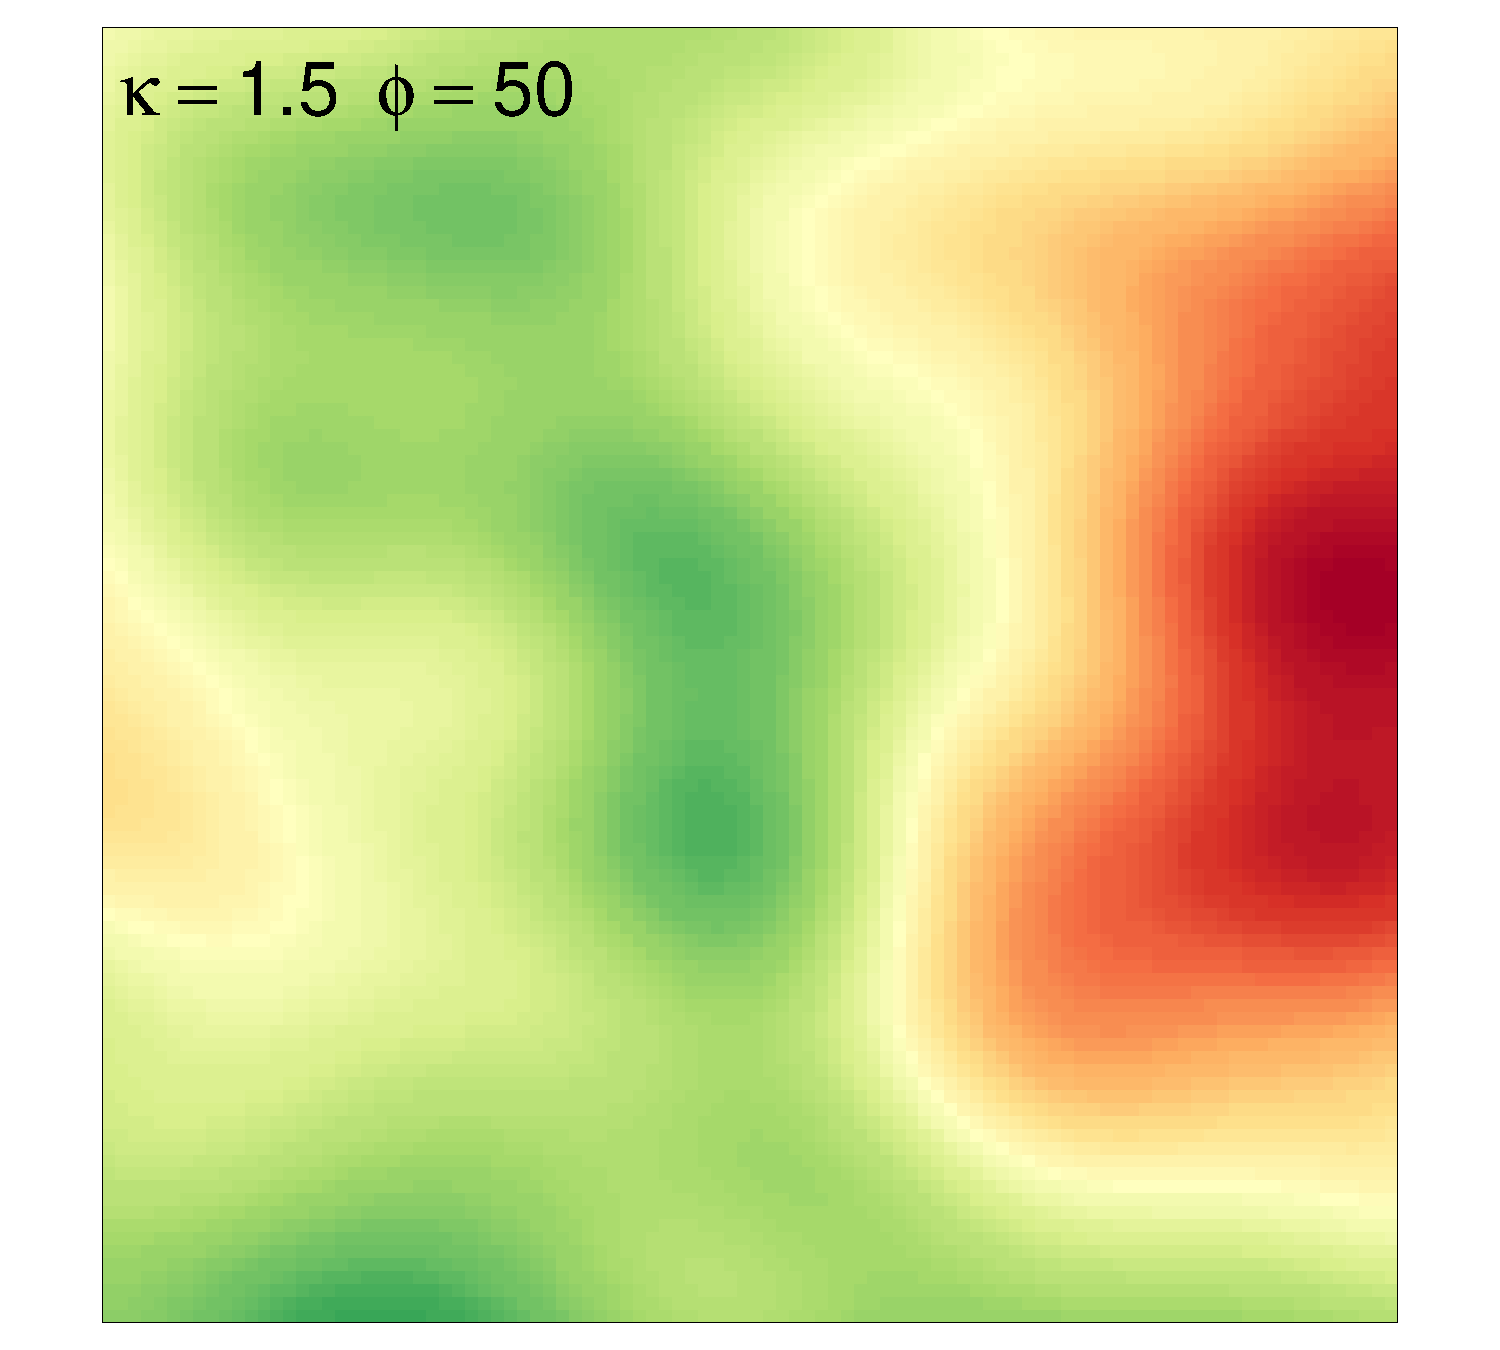
\includegraphics{Lecture_1_files/figure-beamer/unnamed-chunk-37-1.pdf}
\end{column}
\end{columns}
\end{frame}

\hypertarget{matuxe9rn-family-4}{%
\subsection{Matérn family}\label{matuxe9rn-family-4}}

\begin{frame}{Matérn family}
\small

\begin{columns}[T]
\begin{column}{0.33\textwidth}
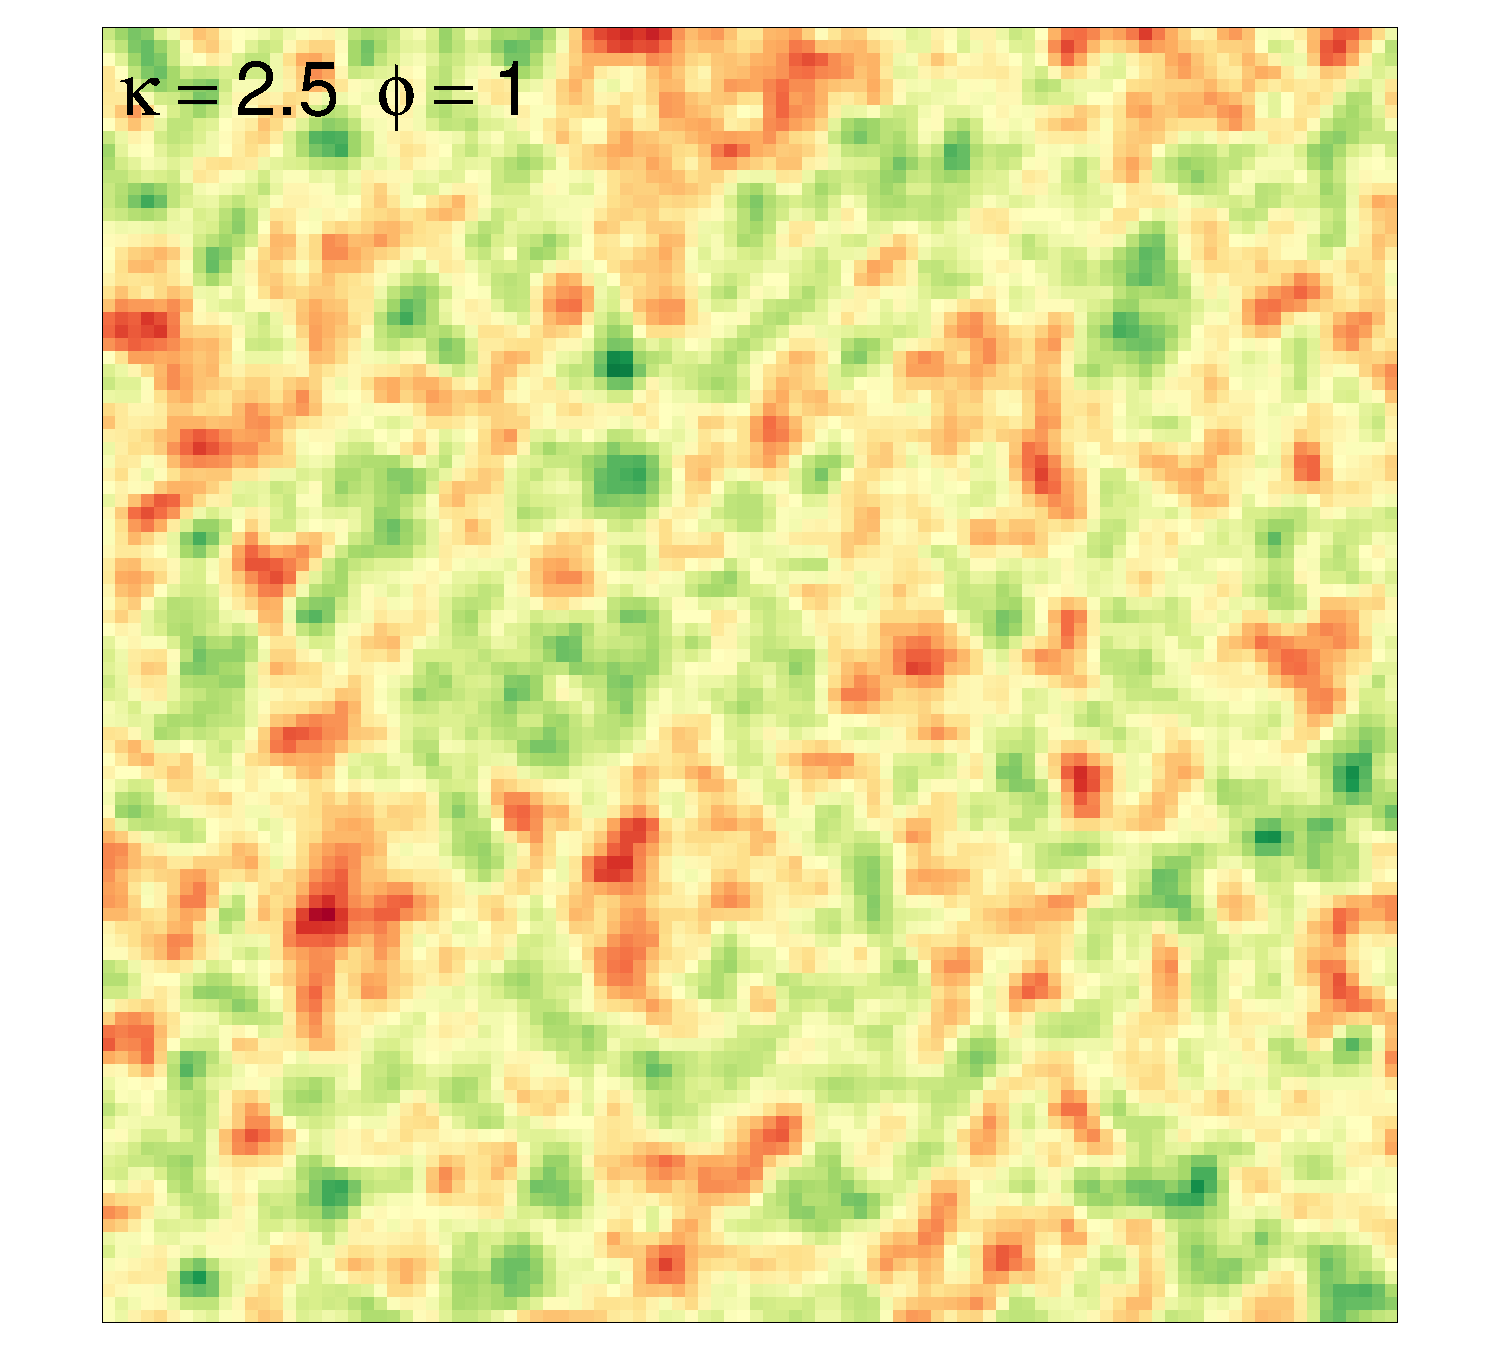
\includegraphics{Lecture_1_files/figure-beamer/unnamed-chunk-38-1.pdf}
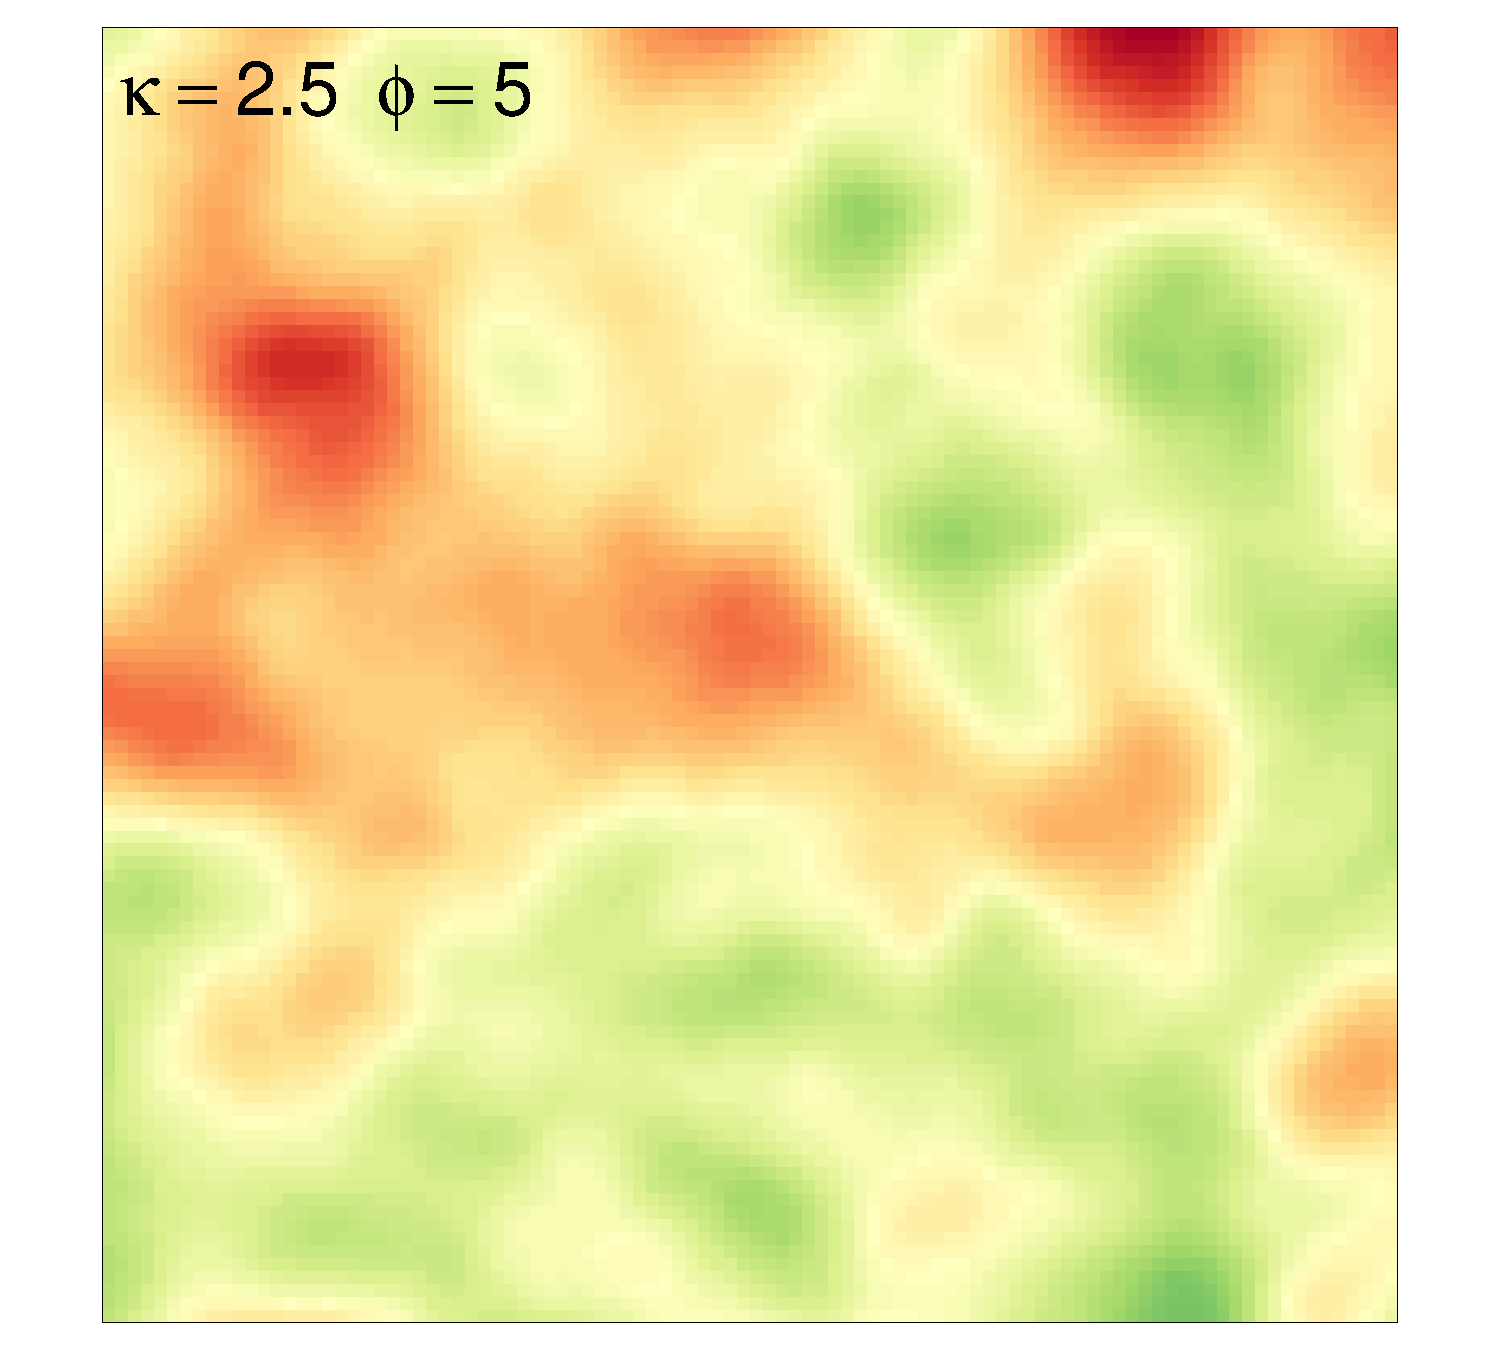
\includegraphics{Lecture_1_files/figure-beamer/unnamed-chunk-39-1.pdf}
\end{column}

\begin{column}{0.33\textwidth}
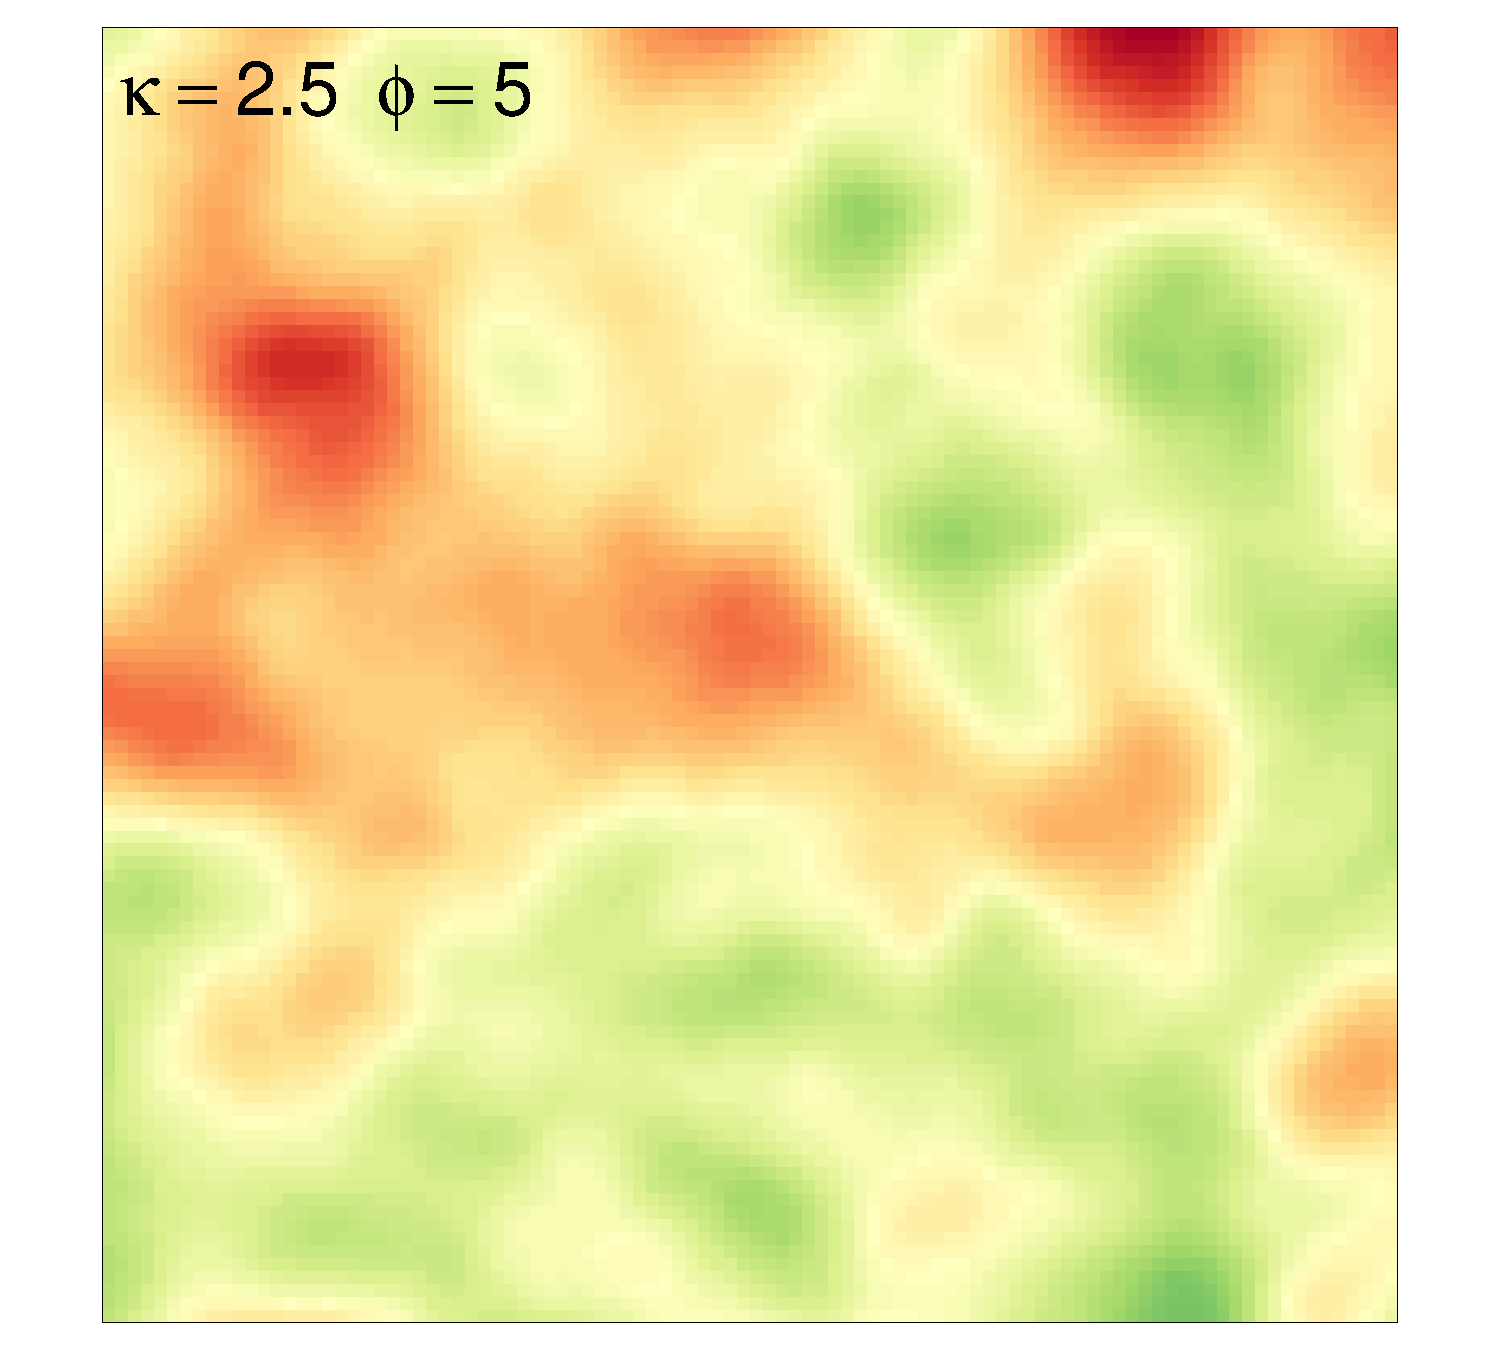
\includegraphics{Lecture_1_files/figure-beamer/unnamed-chunk-40-1.pdf}

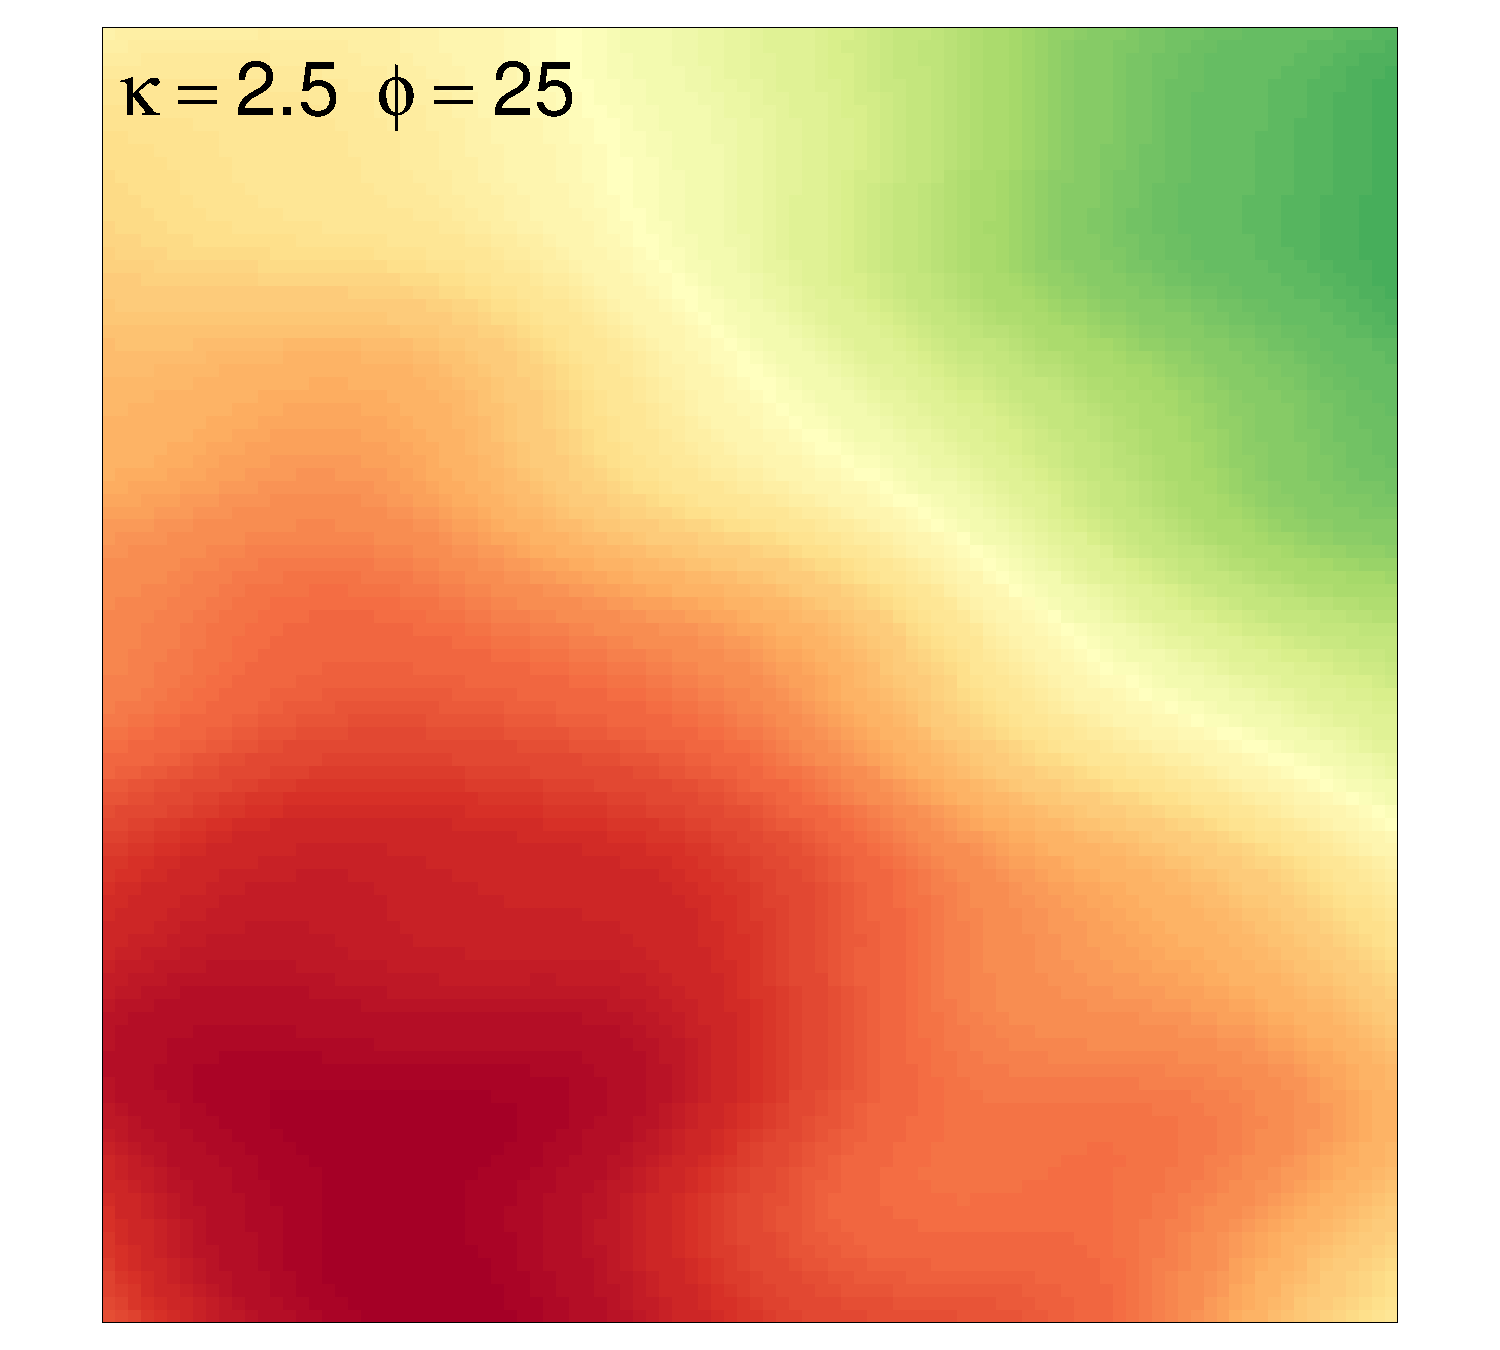
\includegraphics{Lecture_1_files/figure-beamer/unnamed-chunk-41-1.pdf}
\end{column}

\begin{column}{0.33\textwidth}
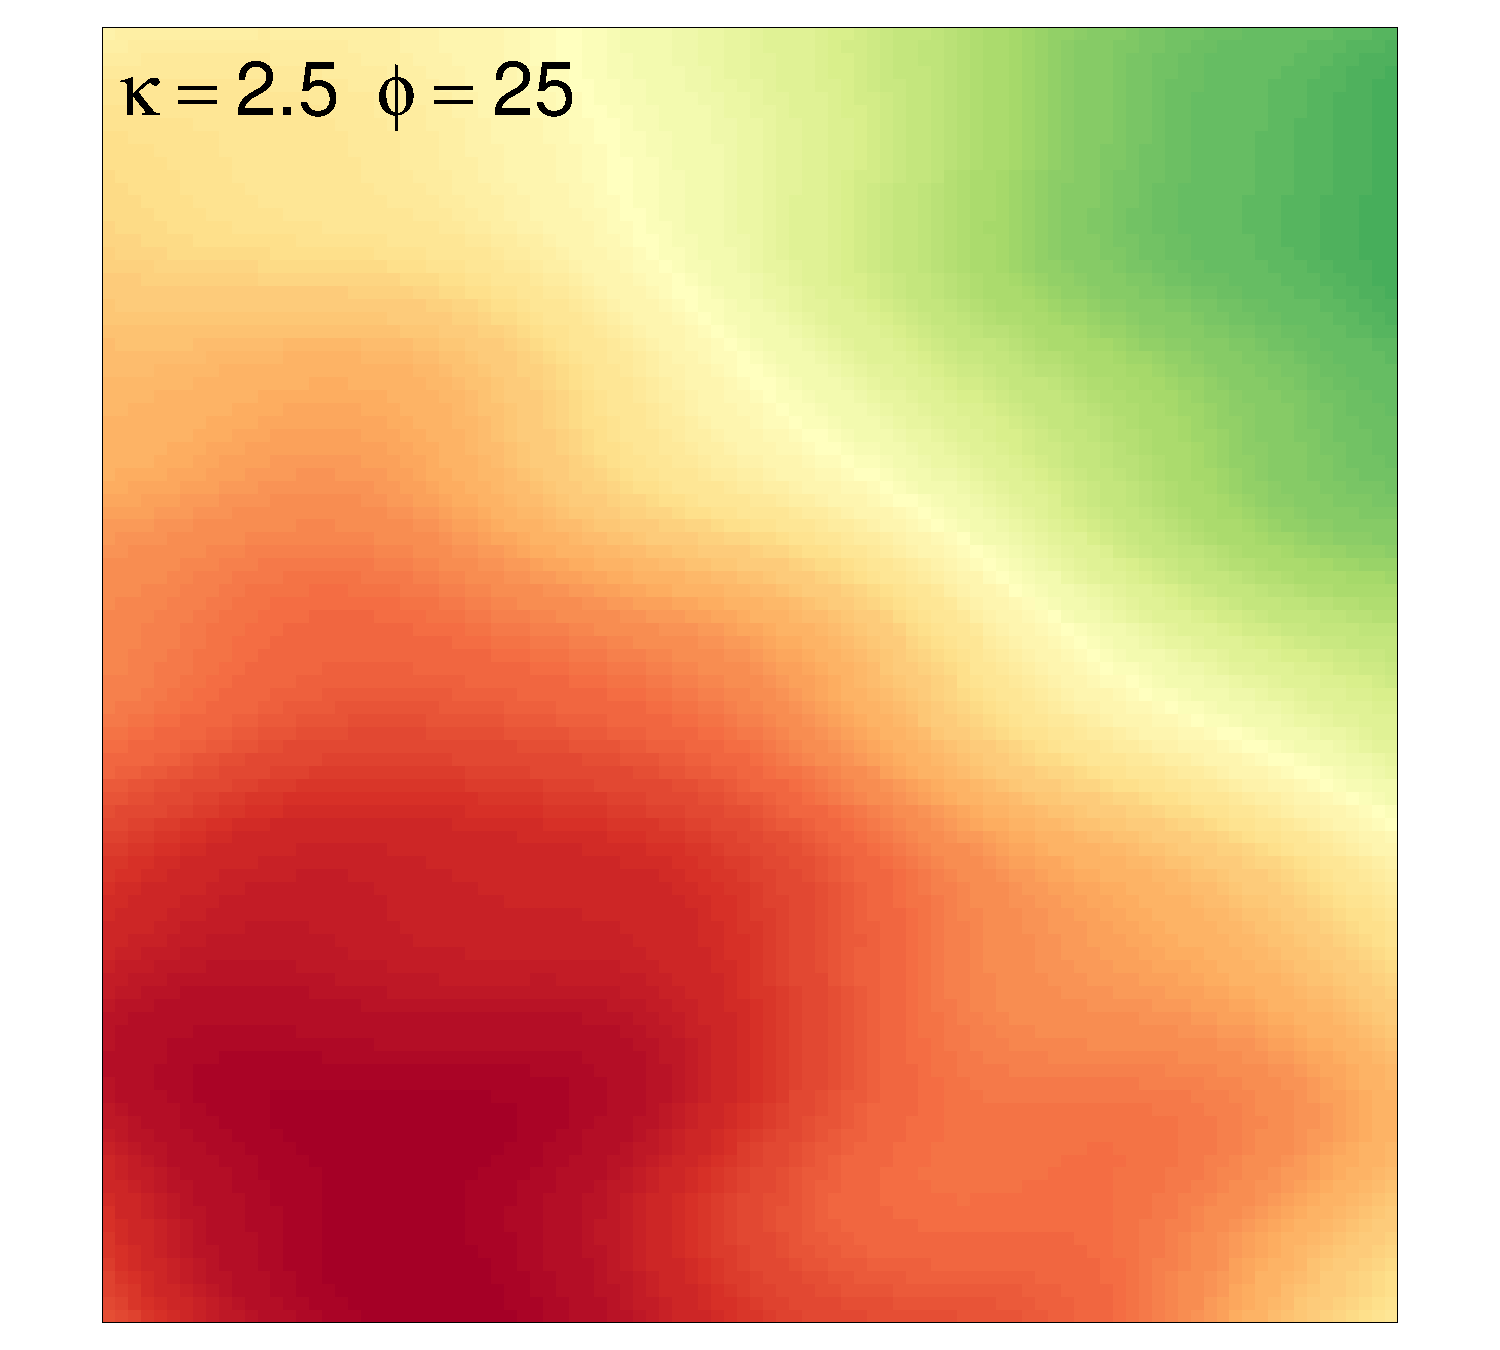
\includegraphics{Lecture_1_files/figure-beamer/unnamed-chunk-42-1.pdf}

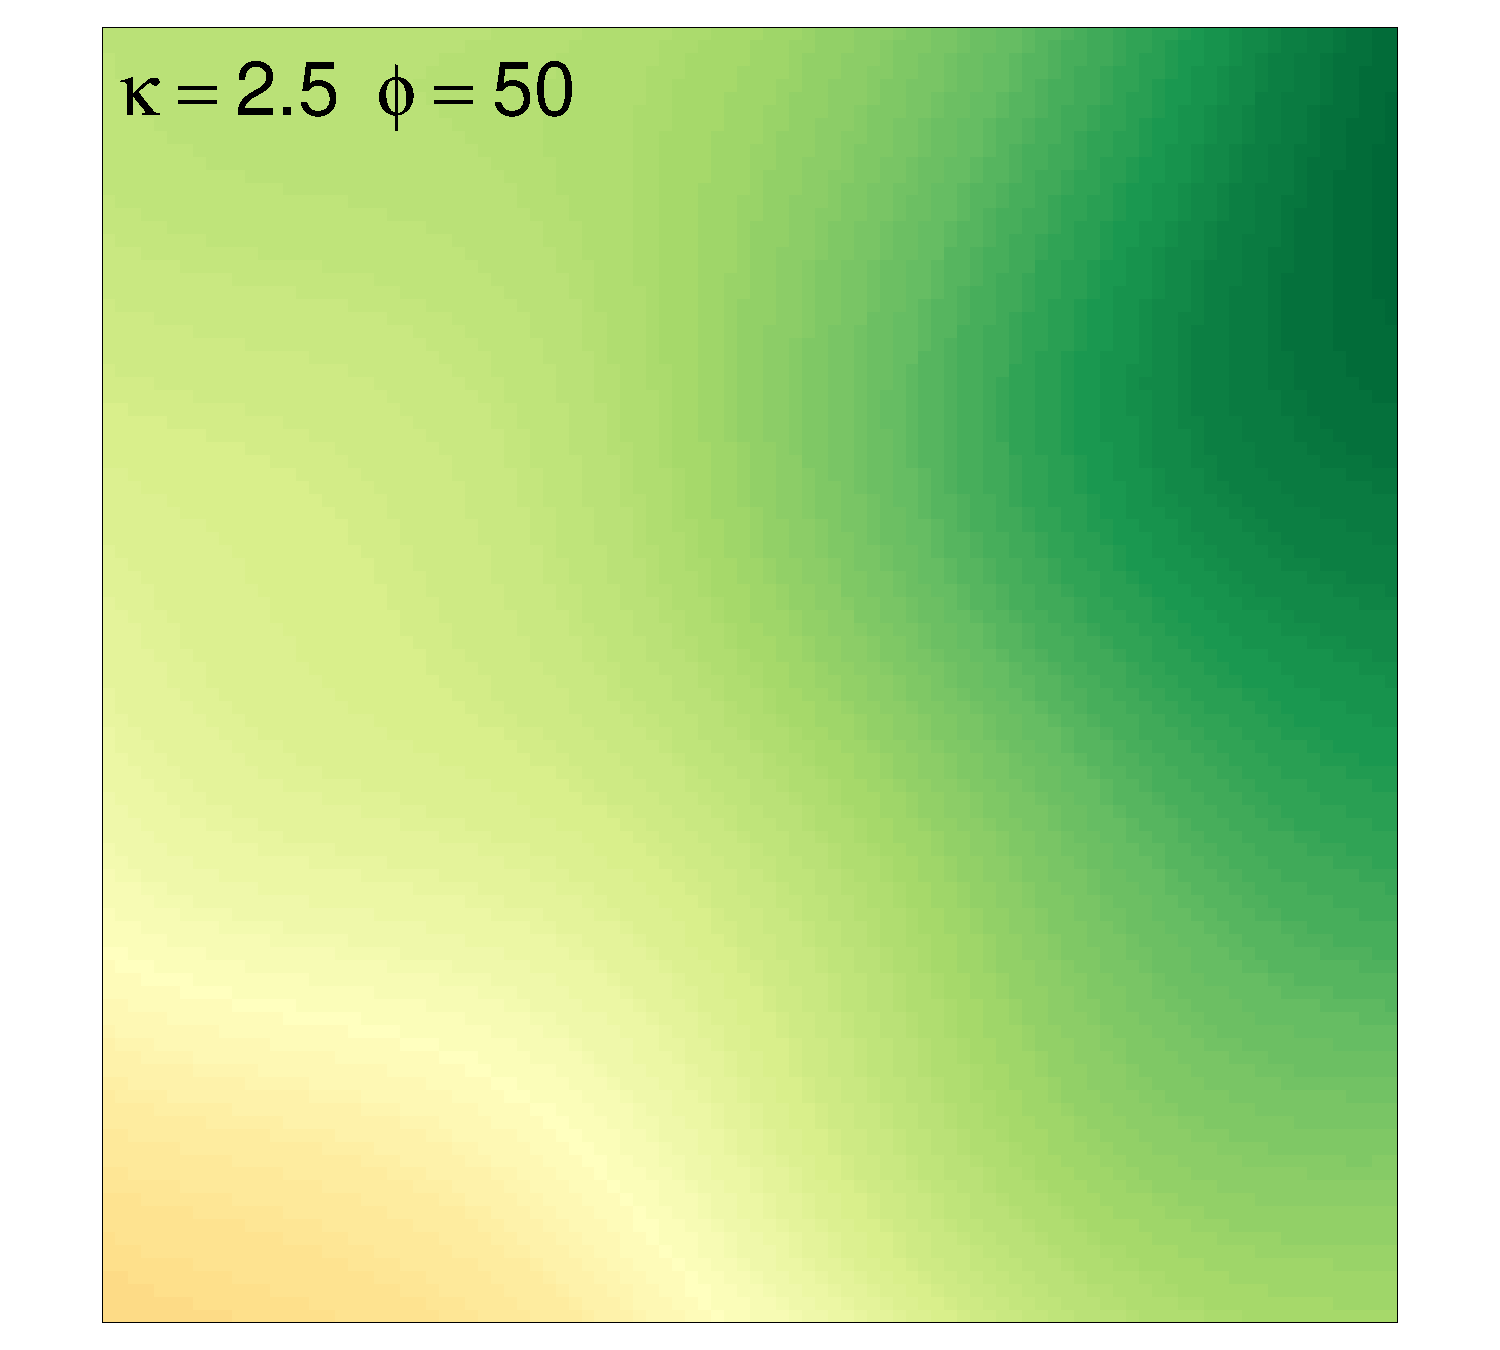
\includegraphics{Lecture_1_files/figure-beamer/unnamed-chunk-43-1.pdf}
\end{column}
\end{columns}
\end{frame}

\hypertarget{spherical-family}{%
\subsection{Spherical family}\label{spherical-family}}

\begin{frame}{Spherical family}
\begin{columns}[T]
\begin{column}{0.5\textwidth}
\small

\[
\rho(u)= \left\{
\begin{array}{ll}
      1-\frac{3}{2}\left(\frac{u}{\phi}\right)+\frac{1}{2}\left(\frac{u}{\phi}\right)^3 & 0\leq u \leq \phi \\
      0 & u > \phi\\
\end{array} 
\right. 
\]

\(\phi\) \ldots{} range, \(\phi>0\)

\includegraphics{Lecture_1_files/figure-beamer/unnamed-chunk-44-1.pdf}
\end{column}

\begin{column}{0.5\textwidth}
\includegraphics{Lecture_1_files/figure-beamer/unnamed-chunk-45-1.pdf}
\includegraphics{Lecture_1_files/figure-beamer/unnamed-chunk-46-1.pdf}
\end{column}
\end{columns}
\end{frame}

\hypertarget{variogram}{%
\section{Variogram}\label{variogram}}

\hypertarget{variogram-1}{%
\subsection{Variogram}\label{variogram-1}}

\begin{frame}{Variogram}
\small

\textbf{(Semi)Variogram} \ldots{} alternative description of the
autocorrelation structure:

\[V(x,x')=\frac{1}{2}Var\left(S(x)-S(x')\right)\]

For stationary isotropic process, it is easy to show that:

\[V(u) = \sigma^2 - C(u)\]

\[V(u)=\sigma^2\left\{1-\rho(u)\right\}\] -\textgreater{} Variogram has
an \emph{inverse shape} compared to the correlation function.
\end{frame}

\hypertarget{variogram-2}{%
\subsection{Variogram}\label{variogram-2}}

\begin{frame}{Variogram}
\small

\begin{columns}[T]
\begin{column}{0.48\textwidth}
Matérn:

\includegraphics{Lecture_1_files/figure-beamer/unnamed-chunk-47-1.pdf}

\includegraphics{Lecture_1_files/figure-beamer/unnamed-chunk-48-1.pdf}
\end{column}

\begin{column}{0.48\textwidth}
Spherical:

\includegraphics{Lecture_1_files/figure-beamer/unnamed-chunk-49-1.pdf}

\includegraphics{Lecture_1_files/figure-beamer/unnamed-chunk-50-1.pdf}
\end{column}
\end{columns}
\end{frame}

\hypertarget{nugget-effect}{%
\subsection{Nugget effect}\label{nugget-effect}}

\begin{frame}{Nugget effect}
\small

Realistic assumption: data \((x_i,y_i)\) are generated by a stationary
``observational'' process

\(Y_i=S(x_i)+\epsilon_i\), where
\(z_i\sim iid, E(z_i)=0, Var(z_i)=\tau^2\)

Variogram is then:

\[V_Y=\tau^2+\sigma^2\left\{1-\rho(u)\right\}\]

\includegraphics{Lecture_1_files/figure-beamer/unnamed-chunk-51-1.pdf}
\end{frame}

\hypertarget{nugget-effect-1}{%
\subsection{Nugget effect}\label{nugget-effect-1}}

\begin{frame}{Nugget effect}
\small

First approach:

\begin{itemize}
\tightlist
\item
  we decide to \emph{model the nugget effect}
\item
  \(\tau^2\) is estimated from data
\item
  two-fold interpretation:

  \begin{enumerate}
  \tightlist
  \item
    measurement error
  \item
    variability of \(S(x)\) in the scale smaller than the scale of the
    measurement
  \end{enumerate}
\item
  cannot be separated, unless we have repeated measurements at the same
  site
\item
  interpolation does not fit the data points precisely
\end{itemize}

Second approach:

\begin{itemize}
\tightlist
\item
  we decide to \emph{set the \(\tau^2=0\) fixly} (no measurement error)
\item
  interpolation exactly fits the data points
\end{itemize}
\end{frame}

\hypertarget{variogram-estimation}{%
\subsection{Variogram estimation}\label{variogram-estimation}}

\begin{frame}{Variogram estimation}
\small

\begin{enumerate}
\tightlist
\item
  Compute \(v_{ij}=\frac{1}{2}\left(Y_i-Y_j\right)^2\)
\item
  Plot \(v_{ij}\) against \(u\) -\textgreater{} \textbf{variogram cloud}
\item
  Smooth out the variogram cloud -\textgreater{} \textbf{empirical
  variogram}
\end{enumerate}

\begin{columns}[T]
\begin{column}{0.48\textwidth}
\includegraphics{Lecture_1_files/figure-beamer/unnamed-chunk-52-1.pdf}
\end{column}

\begin{column}{0.48\textwidth}
\includegraphics{Lecture_1_files/figure-beamer/unnamed-chunk-53-1.pdf}
\end{column}
\end{columns}
\end{frame}

\end{document}
